\section{Timing layers for FCC and jets}
%$Z'\rightarrow WW$  $Z' \rightarrow q\bar{q}$
In the previous sections, the capability of the timing among the various resolutions of the detector used on distinguishing the different kinds of single particle that has the different mass, momentum as well as the length of going through the detector is well-investigated as the excellent variable within the three sigma hypothesis. The next necessary step is to employ the timing, which is the potential method of discriminating the different number of the subjets in a large radius jet as well, into tackling the intractable dilemma that has been being concerned about on the highly-boosted circumstances resulting in the particles of the jet are too close to each other, and the truth number of the subjet could be misestimated, along with impacting on the analysis in the future dramatically.\\ 

The simplified-cases simulating the pileup-free conditions with the already-known processes are involved in these studies under the environment of a very-high-energy collider will be explored as the benchmark of the timing applied in the future. The same processes of Z'$\rightarrow$qq(Background), Z'$\rightarrow$WW(Signal) with 5, 10, 20 and 40TeV center-of-mass energy(C.M.) as the ones exploited in our second paper, are taken into account as the targets of doing the researches on the same matter with the timing implemented.\\ 
%adopting the jet-substructure variables to deal with estimating the internal structure of the boosted jets for those processes

In terms of digging out the potential of the timing, several studies have been done trying on a couple of variables to see whether the timing can give us another degree of information helping on having the improvement on the issue in addition to the $P_{T}$ that we could obtain directly from the detector . The $\Delta R$, which is the common variable that has been being used in the collider as acquiring the angle between two particles/jets, is found to be the possible one that can take advantage of using the timing to analyze the structure of the jets more evidently. Also, the ideal cases of separating the different particles with the help of the timing are also premeditated.\\

The two sets of the collections of the data including both of the generator level(truth-level) and the reconstruction level(reco-level) are utilized in the studies for the purpose of corresponding between each other as the benchmark of the parameters that are found beneficial. At the first place, the definition of many terms applied in the studies will be well-defined as a favor of proceeding smoothly. The second one is to make use of the truth-level information of the four momenta for each particle to figure out the anticipation of the timing being capable of helping on the issue at best ideally. Last but not least, the well-established cases illustrated by using the reco-level information of the non-smearing four momenta and the fastest-response timing\footnote{As a matter of fact that the detector can response to the first-arrival particle barely in one event, the timing observed from the reco-level can merely be treated as the part of the jet but not the whole one. Oppositely, the particles of the four momenta from a jet can be explicitly known from the information of the truth-level, and the timing of each particle should be well-calculated with the formula of the timing listed in the following sections as the ideal cases.} from each cell of the calorimeter will be given as the true cases we could expect in our life when the time of the timing-capable detector installed in the collider with the very high C.M. energy comes.\\

\subsection{The definitions of the terms introduced in the following studies}
\label{sec:Def_timing}
In case for avoiding being confused by the terms applied in these studies, pre-defining for those terms is essential.\\
\subsubsection{The timing used in the truth-level cases}
At the first place, the definition of the timing should be obtained as our benchmark to do these studies when dealing with the truth-level information. The standard formula of the timing is as follows for each particle:
\begin{equation}
 Timing = \frac{L(\eta)}{V(V_{x},V_{y},V_{z})}  
\end{equation}

Basically, it is the normal formula of the time of flight(TOF), depending on the different \(\eta\), leading to the different distances\(\ L\) between collision point and HCAL barrel, along with the three-dimensional velocities\(\ V \) of the particles.\\

But, since the effect of the magnetic field is taken into account, the timing applied in this paper is the modified one with only considering the Z direction of the distance and velocity, and then we can get more precise value of the timing by the truth of the Z-direction trace of the particle isn't changed by the magnetic field. The formula used in this paper is as follows: 

\begin{equation}
 Timing = \frac{L_{z}}{V(V_{z})} 
\end{equation}

After applying this formula on all particles, and the timing can be obtained without the bending effect coming from the magnetic field.\\ 

\subsubsection{The trailing particles applied in all cases}
The another terms should be noticed as the important ones are two sorts of the trailing particles applied in all cases. The definition of the trailing particles defined by the Timing(T) and transverse momentum(PT) should be clarified. We have two categories of the trailing particles
\begin{enumerate}
\item Defined by the T, so-called "trailing-T", meaning that the particle has the longest traveling timing in the jet. 
\item Defined by the PT, so-called "trailing-$P_{T}$", meaning that the lowest-PT particle in the jet. 
\end{enumerate}

Subsequently, we can define the next-to trailing particle as well, such as the second long traveling timing-"next-to-trailing-T"(The second trailing-T) or the second low PT-"next-to-trailing-$P_{T}$"(The second trailing-$P_{T}$), and so on. The order of the trailing particle will be well-specified in the following section.

\subsection{The truth-level cases}
%When coming up with any new variable, the truth-level information can be utilized as the guardian monitoring on the variables could be useful or not without the joint of the particle-showering effect involved in. In this section, the truth-level information will be adopted as the one to aim inspecting the power of the variable found to be the useful one.\\
In order to compare the studies carried out by the truth-level information with the ones done at the reco-level, the selection of the events at the generator level should be enlightened at first. At the first place, since the information of the four momenta upon the particles reconstructed by HCAL barrel in SiFCC will be utilized as the candidates of excavating the potential of the timing, the pre-selection of the eta on the particles should be aligned with the HCAL which is in the region of  $1<| \eta |<2$. Subsequently, the effect of the magnetic field should be concerned as the probably authentic situation occurring in the collider. With the calculations played out by $P_{T}=0.3RT$, the cut down limit of the energy owned by the particles is about 1.5GeV.\\     

With the necessary selection applied on, the advantageous of the $\Delta R$ can be probed thoroughly. Figure \ref{fig:Truth_dR_Dis_5TeV_PT} to Fig.\ref{fig:Truth_dR_Dis_40TeV_T} show some of the distributions of $\Delta R$, which are the angles between the Leading-$P_{T}$ particle and two sorts of trailing particles up to the fifth order, demonstrated by resonance masses of 5TeV and 40TeV individually as two extreme cases explaining on the discriminations phenomenologically. The power of $\Delta R$ applied to discern the jets containing the various number of the subjets is displayed off obviously with those plots.\\

\begin{figure}
\begin{center}
   \subfigure[The first trailing-$P_{T}$] {
   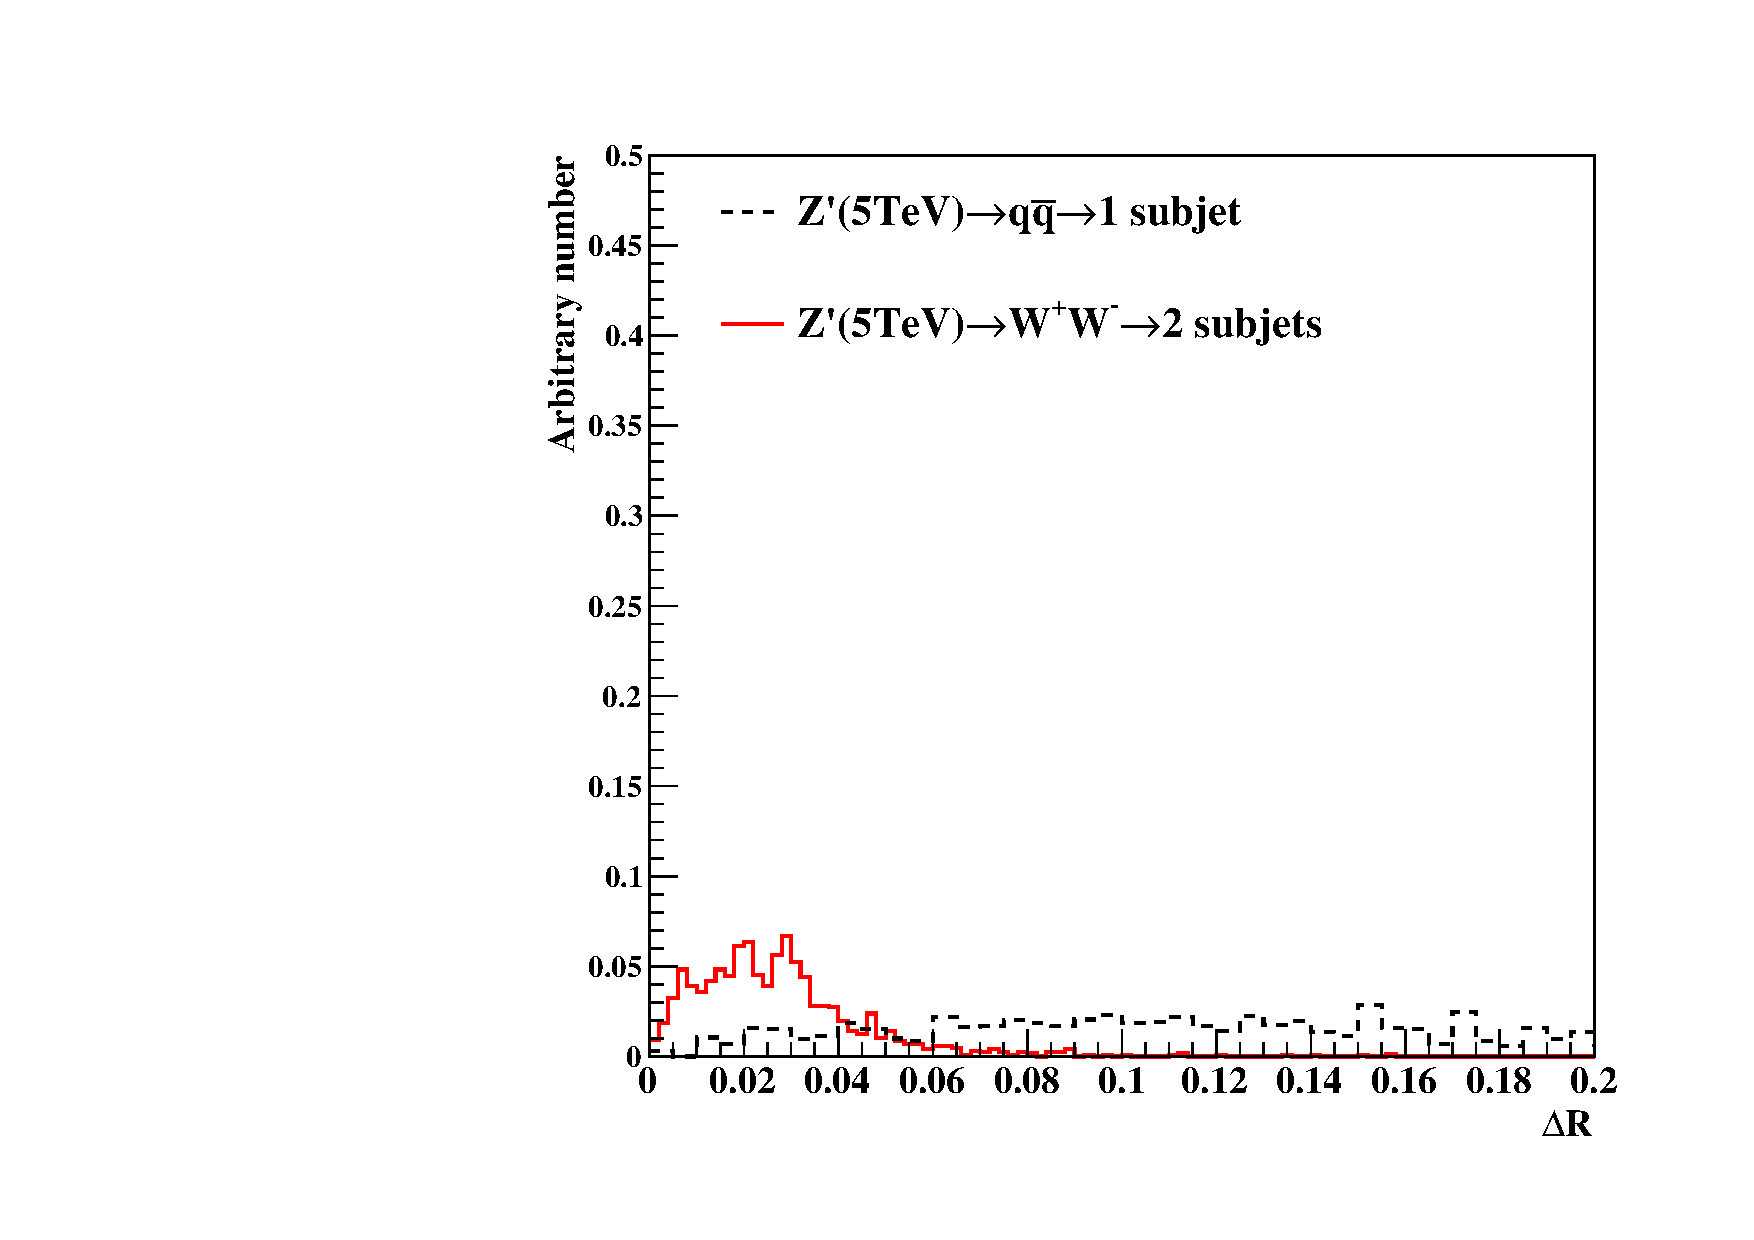
\includegraphics[width=0.3\textwidth]{/Users/ms08962476/Timing_paper/Pictures_used_for_FCC_and_jets/Truth_dR_Dis/5TeV/dR_PT_0_5TeV_Truth.pdf}
   }
   \subfigure[The second trailing-$P_{T}$] {
   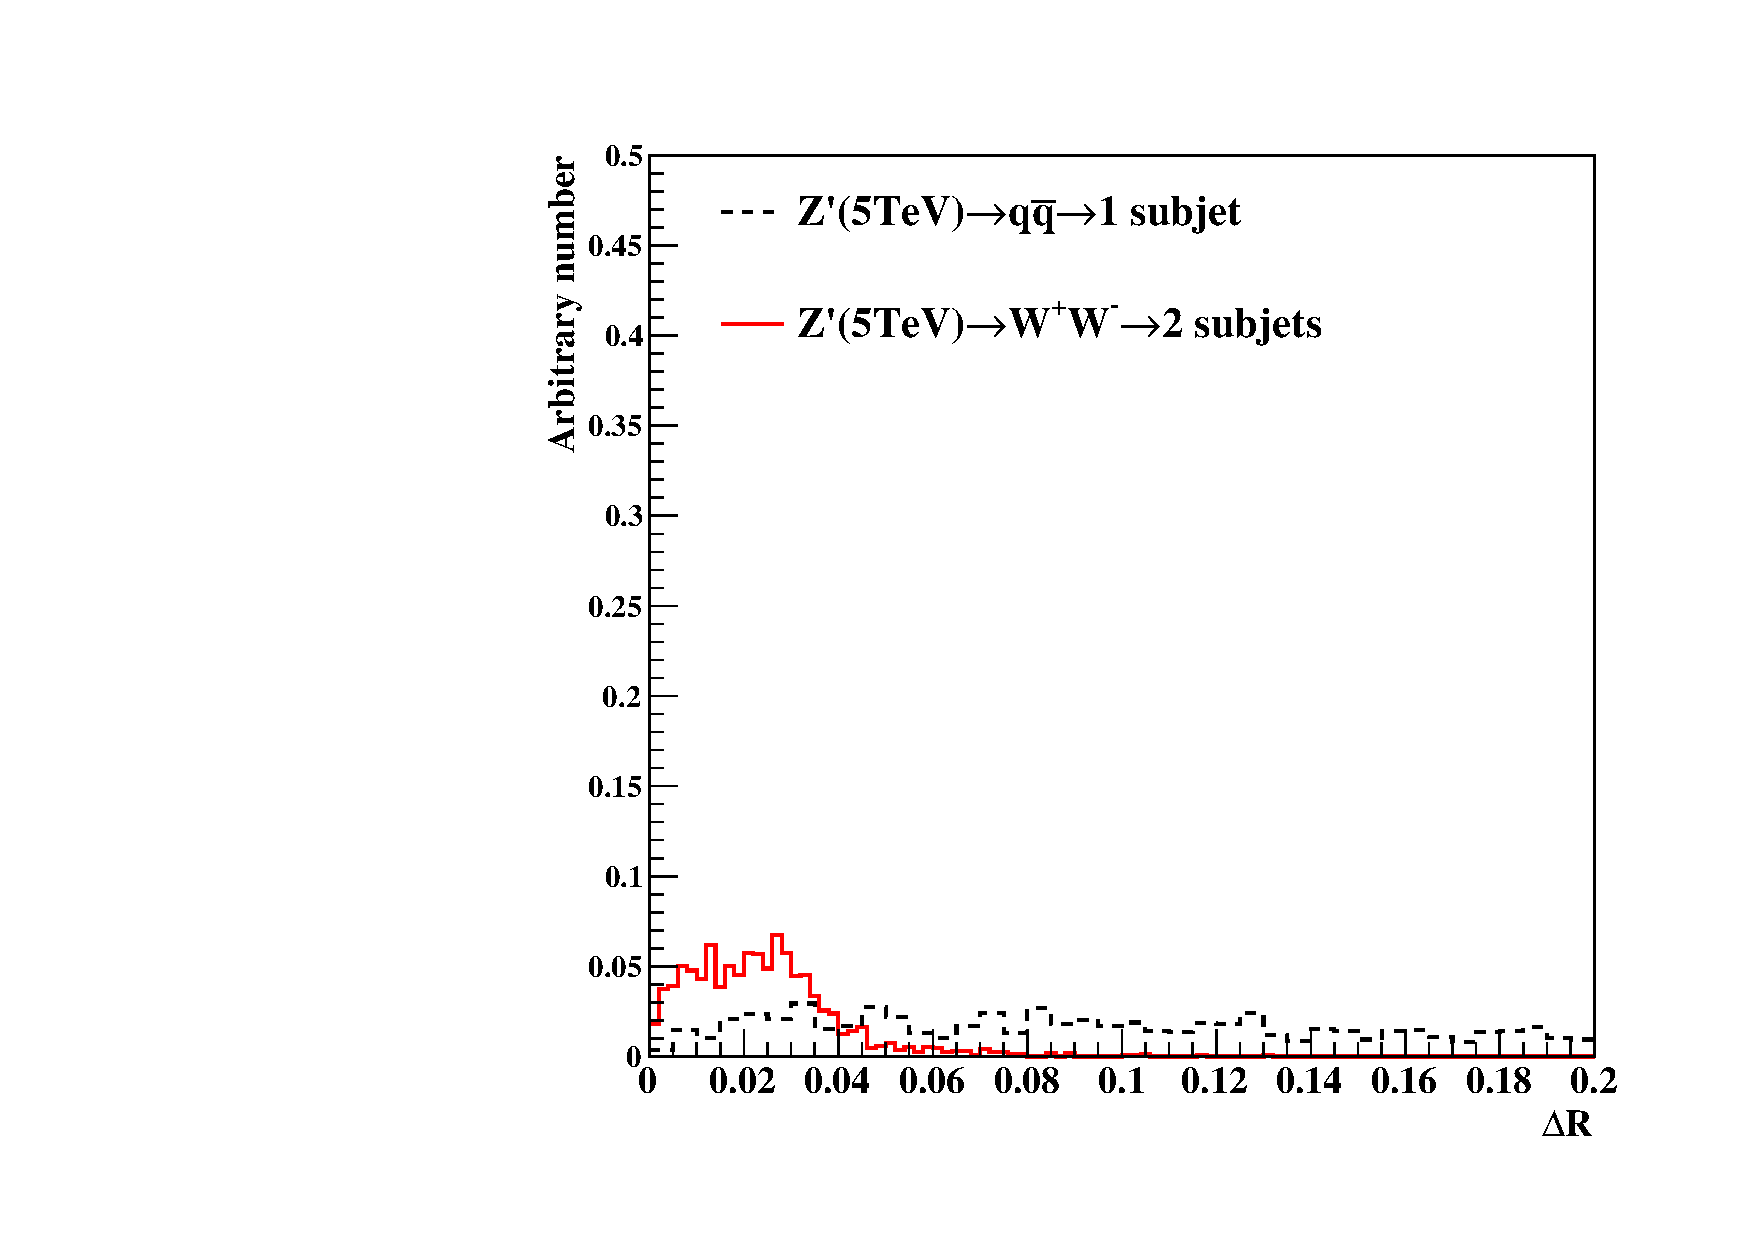
\includegraphics[width=0.3\textwidth]{/Users/ms08962476/Timing_paper/Pictures_used_for_FCC_and_jets/Truth_dR_Dis/5TeV/dR_PT_1_5TeV_Truth.pdf}
   }
   \subfigure[The third trailing-$P_{T}$] {
   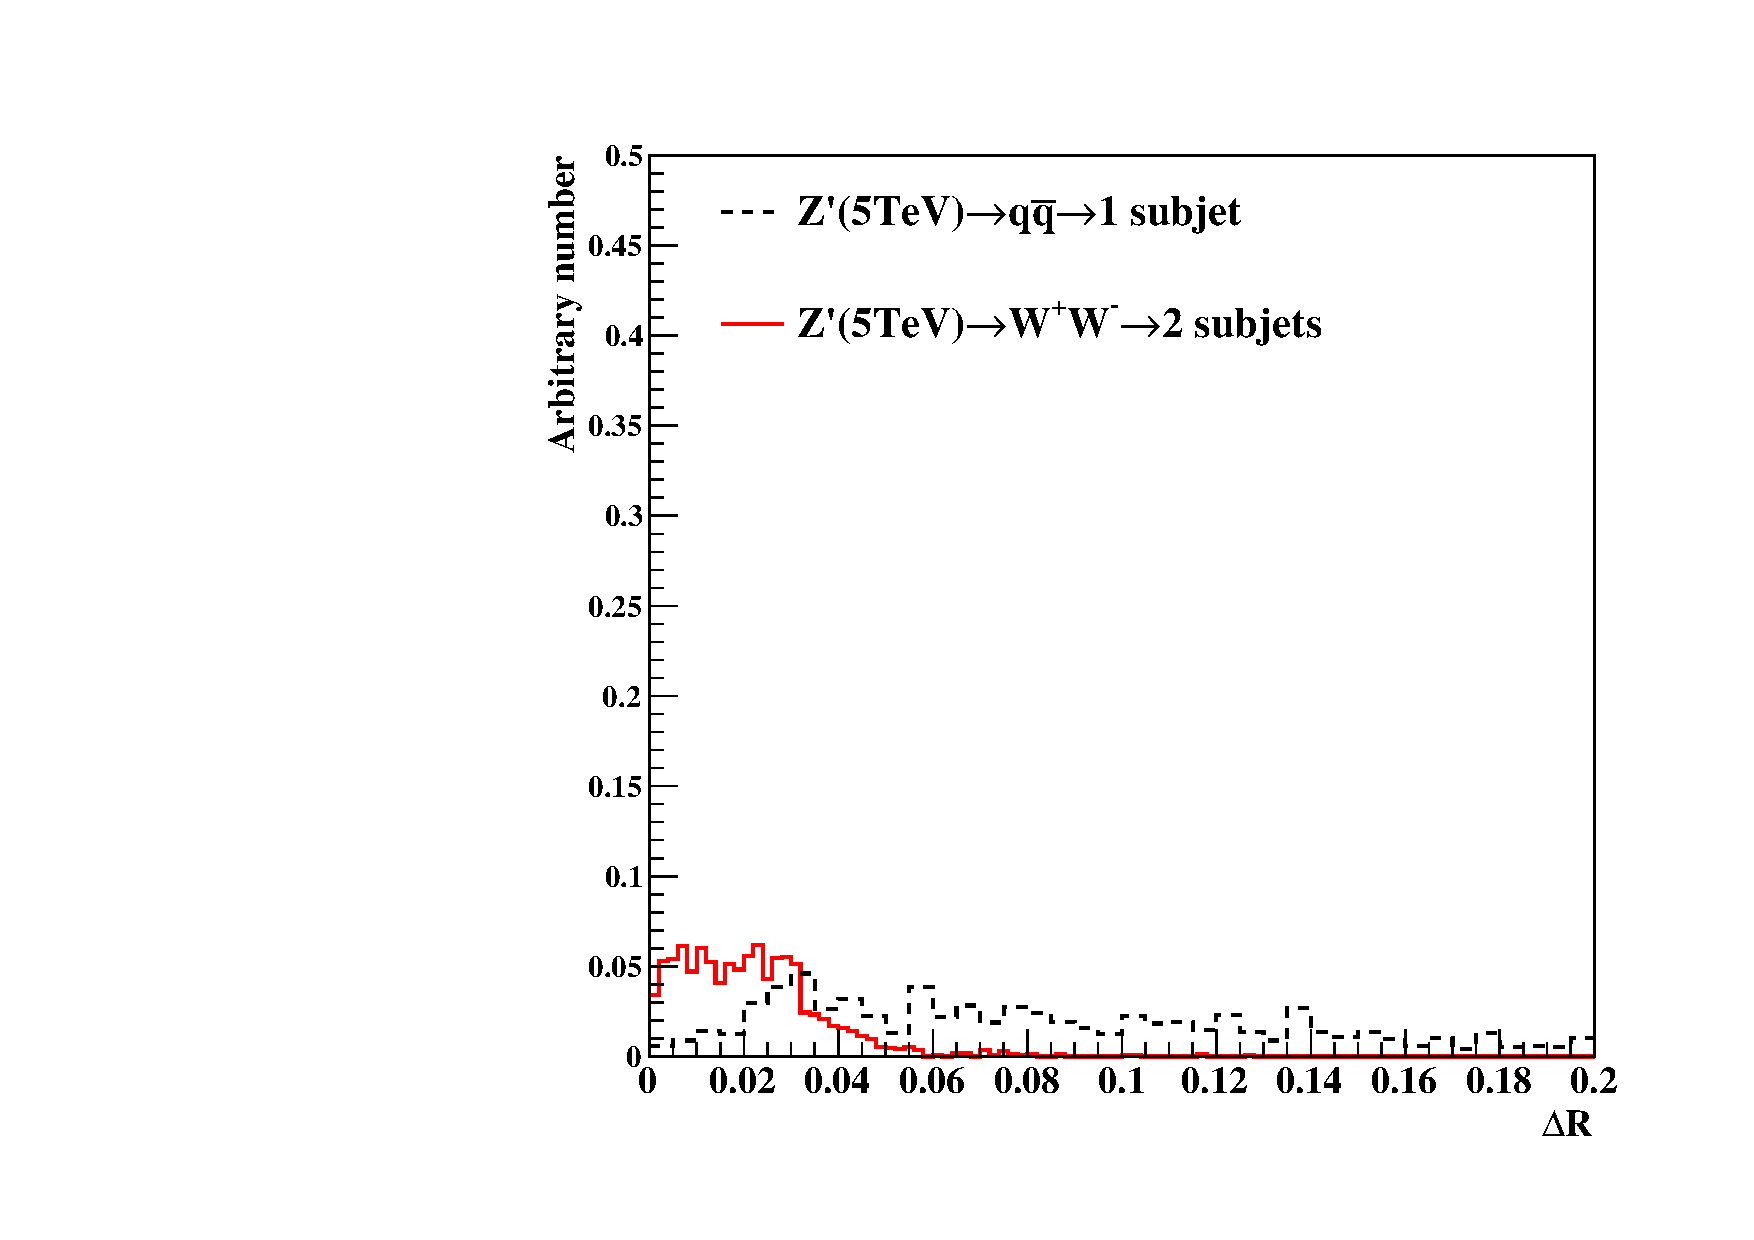
\includegraphics[width=0.3\textwidth]{/Users/ms08962476/Timing_paper/Pictures_used_for_FCC_and_jets/Truth_dR_Dis/5TeV/dR_PT_2_5TeV_Truth.pdf}
   }
      \subfigure[The fourth trailing-$P_{T}$] {
   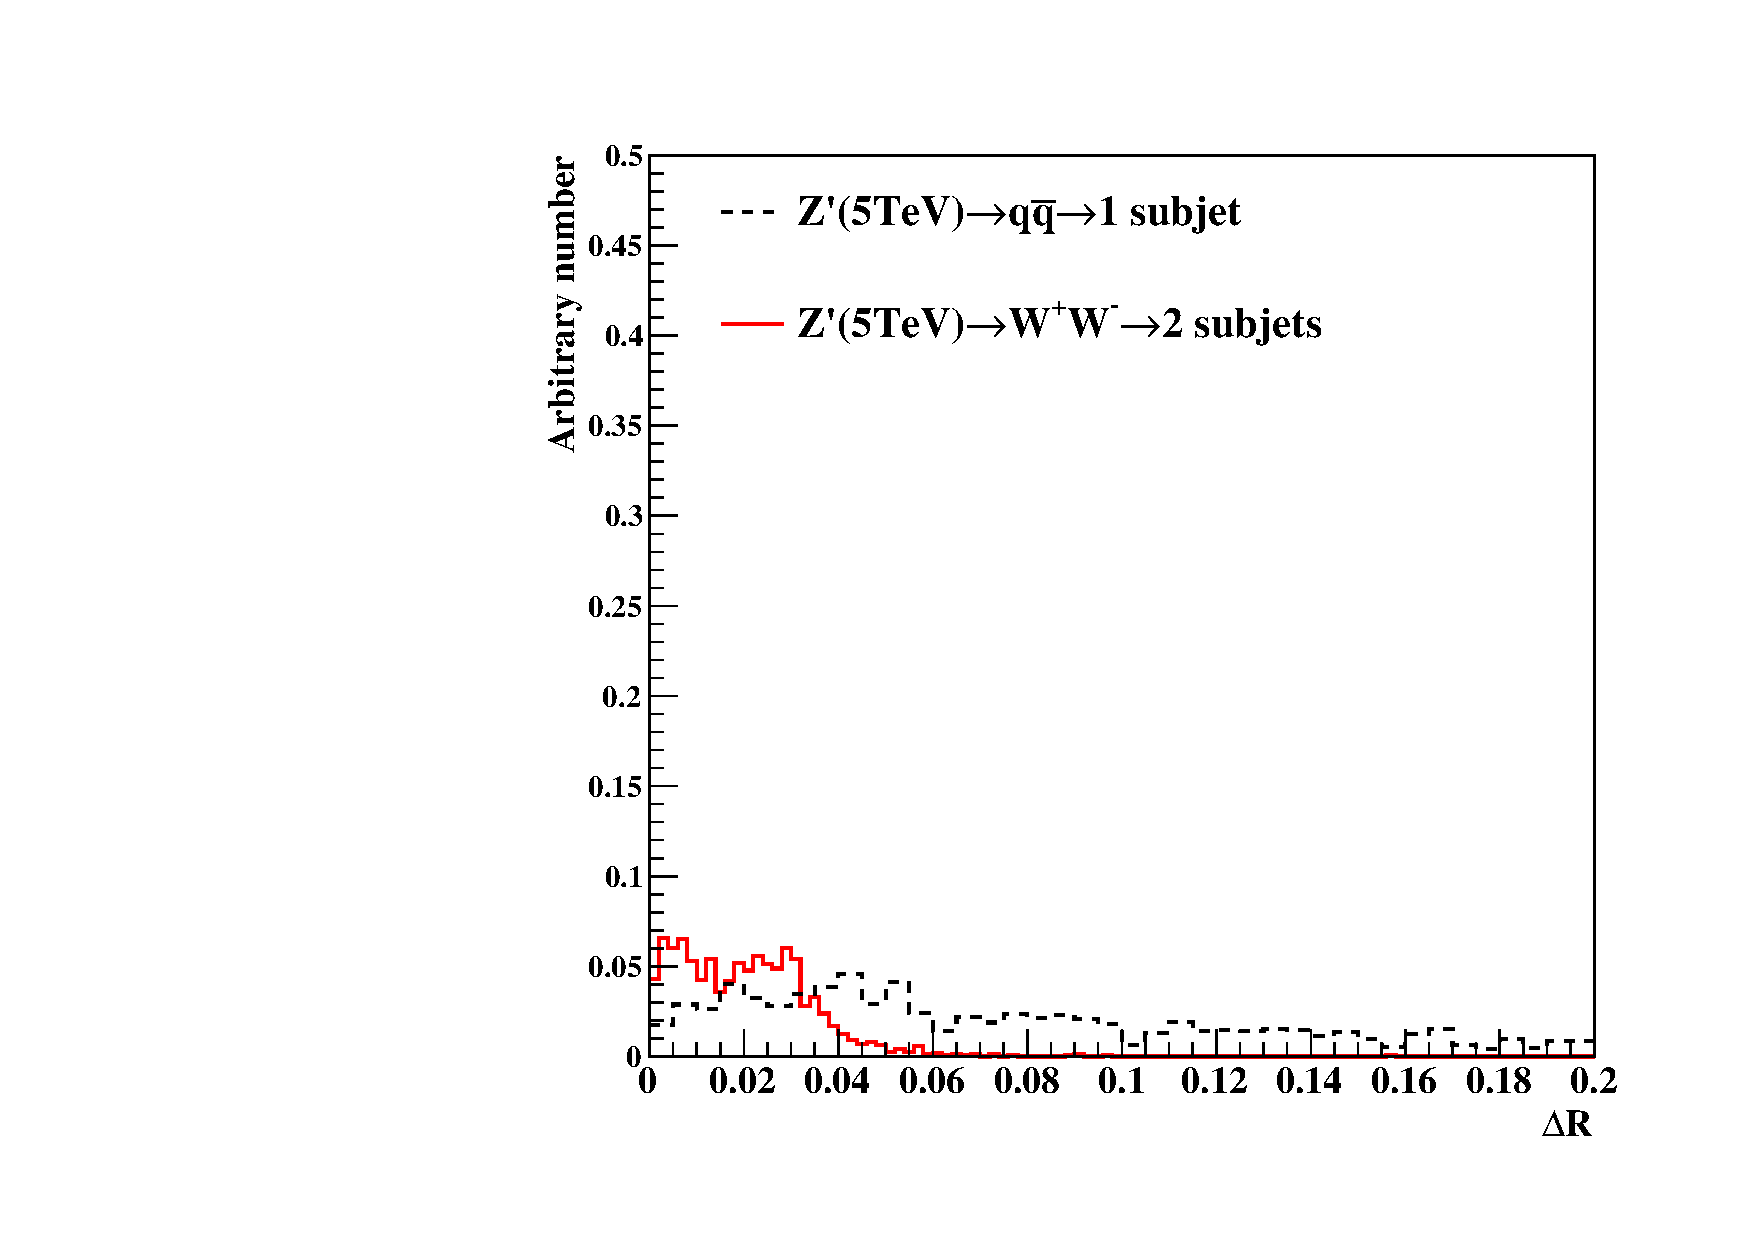
\includegraphics[width=0.3\textwidth]{/Users/ms08962476/Timing_paper/Pictures_used_for_FCC_and_jets/Truth_dR_Dis/5TeV/dR_PT_3_5TeV_Truth.pdf}
   }
   \subfigure[The fifth trailing-$P_{T}$] {
   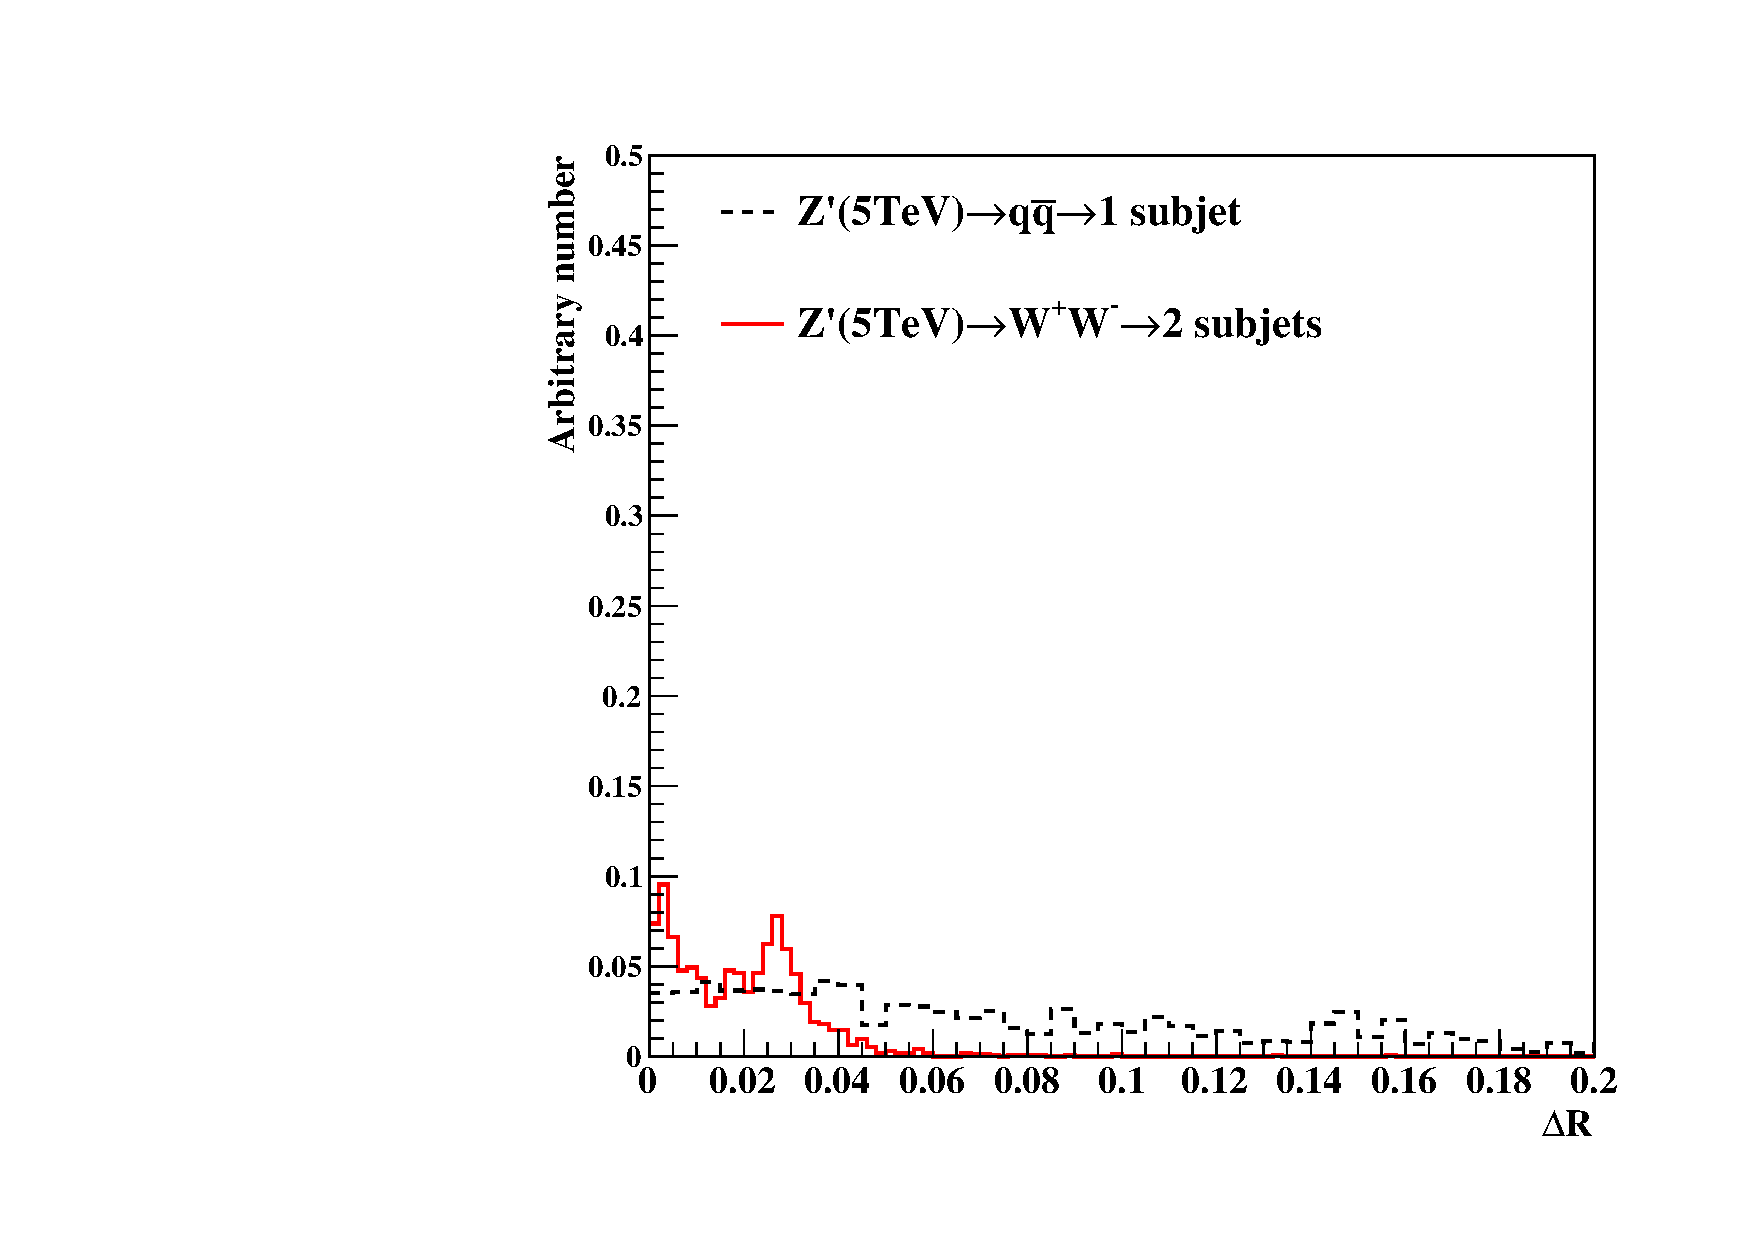
\includegraphics[width=0.3\textwidth]{/Users/ms08962476/Timing_paper/Pictures_used_for_FCC_and_jets/Truth_dR_Dis/5TeV/dR_PT_4_5TeV_Truth.pdf}
   }
\end{center}
\caption{Distributions of $\Delta R$ for $M(Z') = 5$~TeV for five kinds of trailing-$P_{T}$ particles with the truth-level information 
are shown here. \label{fig:Truth_dR_Dis_5TeV_PT}}
\end{figure}

\begin{figure}
\begin{center}
   \subfigure[The first trailing-T] {
   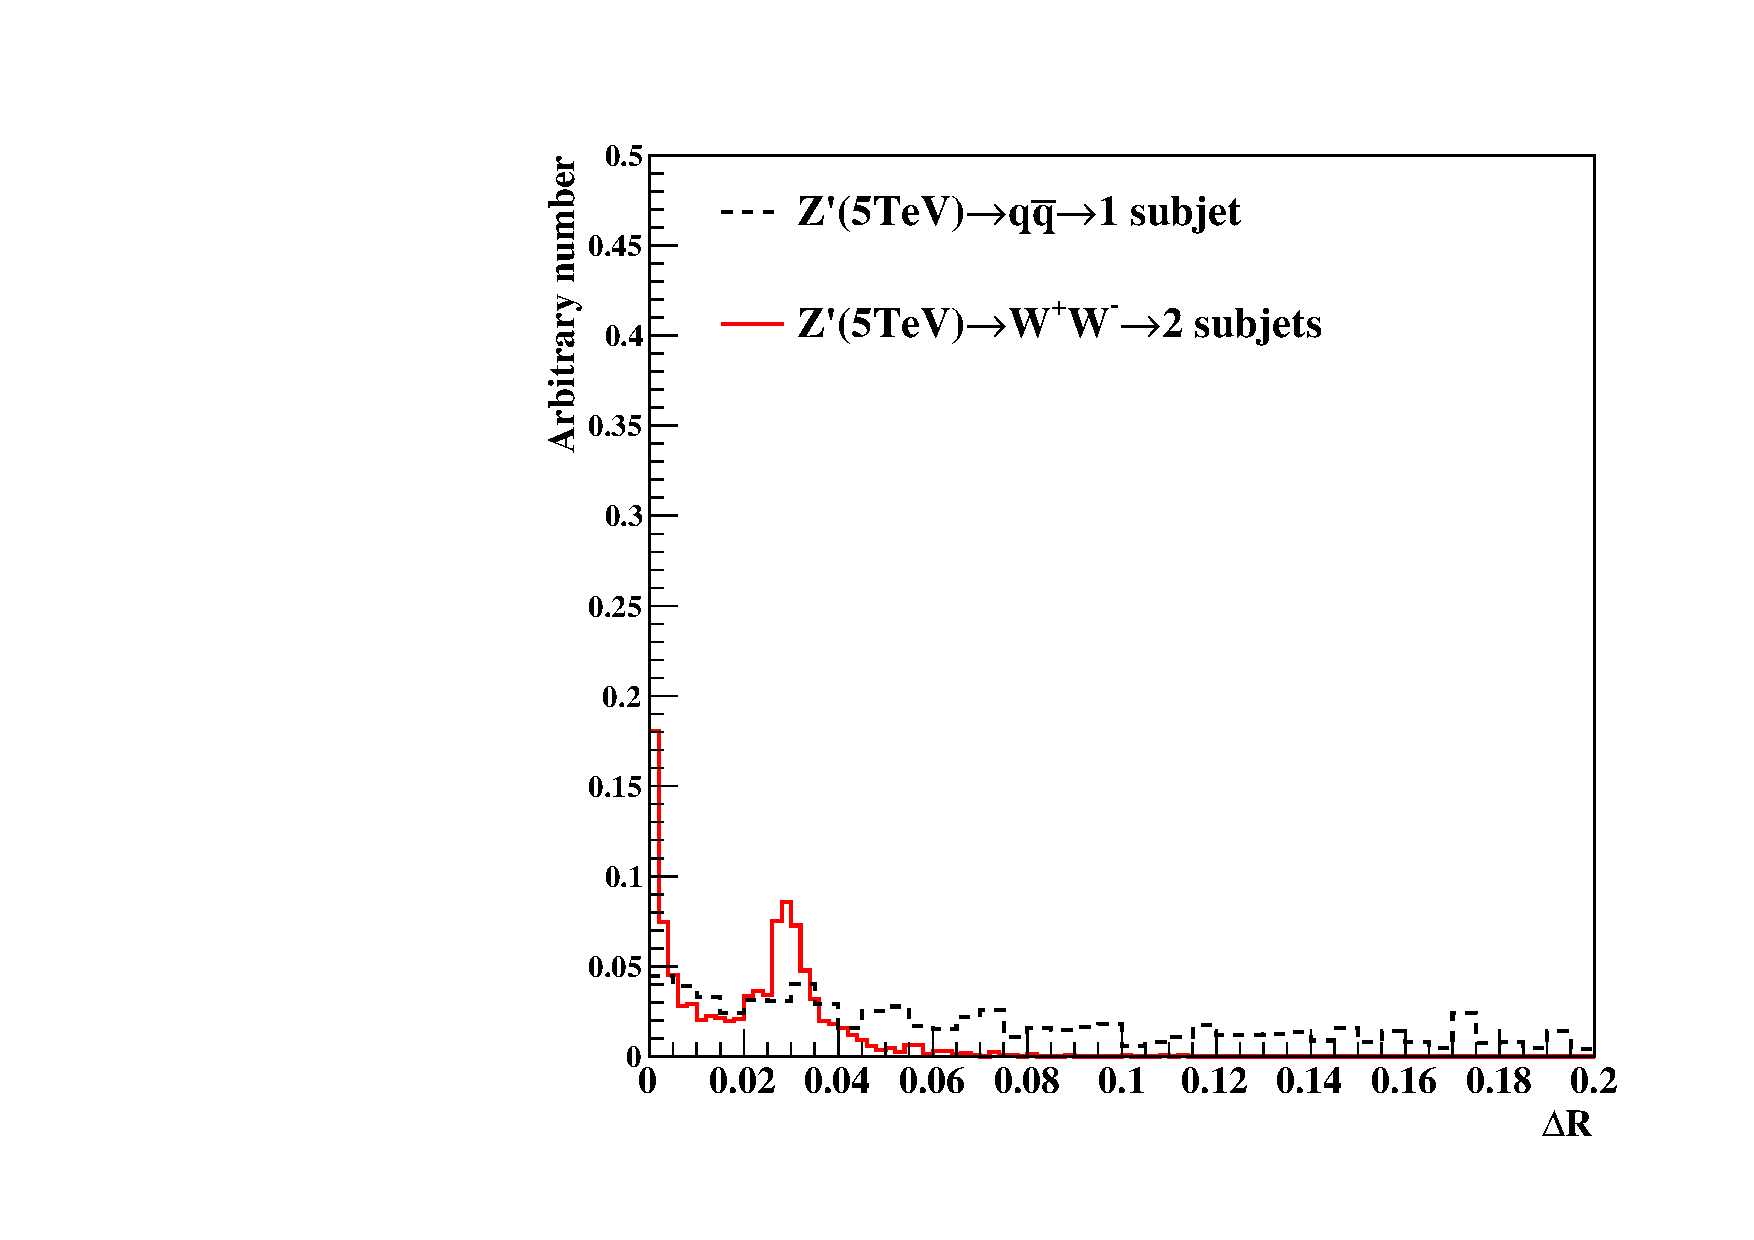
\includegraphics[width=0.3\textwidth]{/Users/ms08962476/Timing_paper/Pictures_used_for_FCC_and_jets/Truth_dR_Dis/5TeV/dR_T_0_5TeV_Truth.pdf}
   }
   \subfigure[The second trailing-T] {
   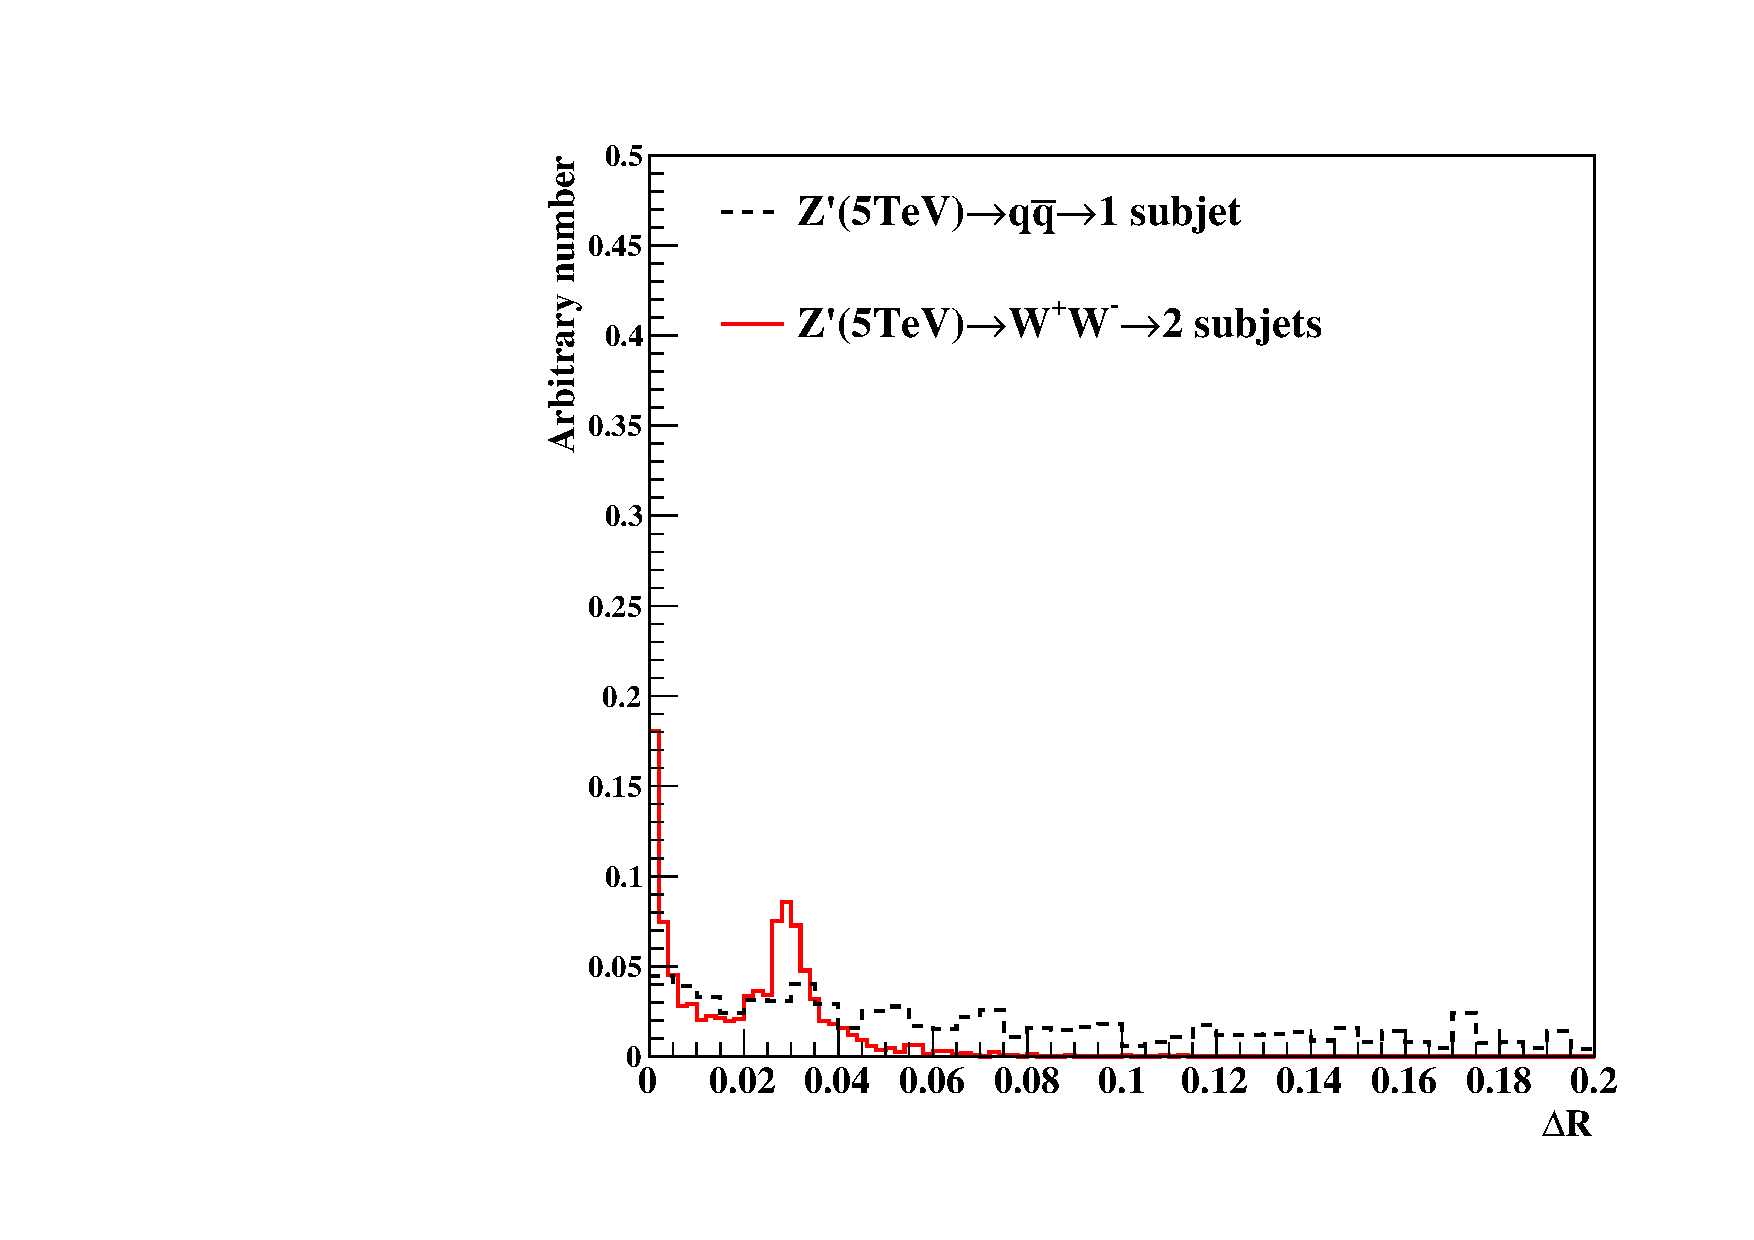
\includegraphics[width=0.3\textwidth]{/Users/ms08962476/Timing_paper/Pictures_used_for_FCC_and_jets/Truth_dR_Dis/5TeV/dR_T_1_5TeV_Truth.pdf}
   }
   \subfigure[The third trailing-T] {
   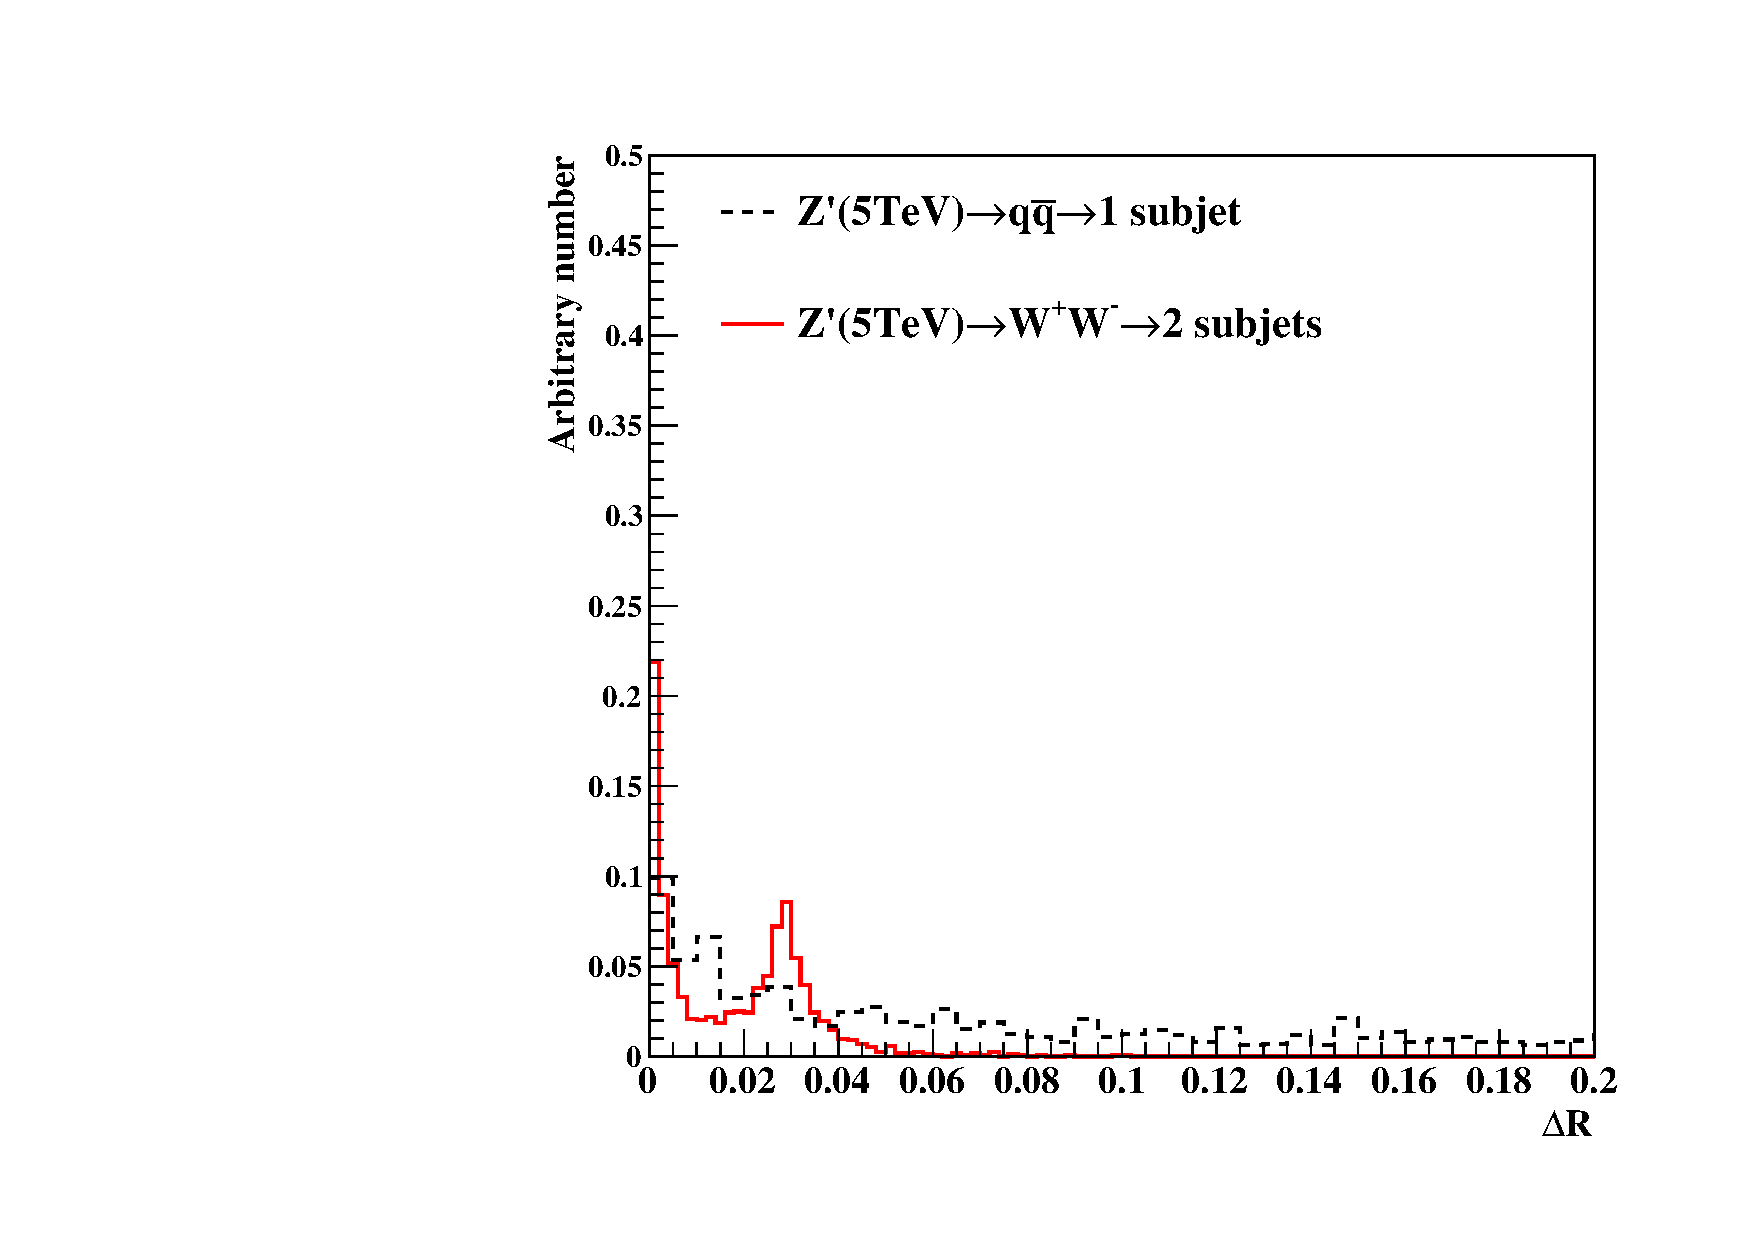
\includegraphics[width=0.3\textwidth]{/Users/ms08962476/Timing_paper/Pictures_used_for_FCC_and_jets/Truth_dR_Dis/5TeV/dR_T_2_5TeV_Truth.pdf}
   }
   \subfigure[The fourth trailing-T] {
   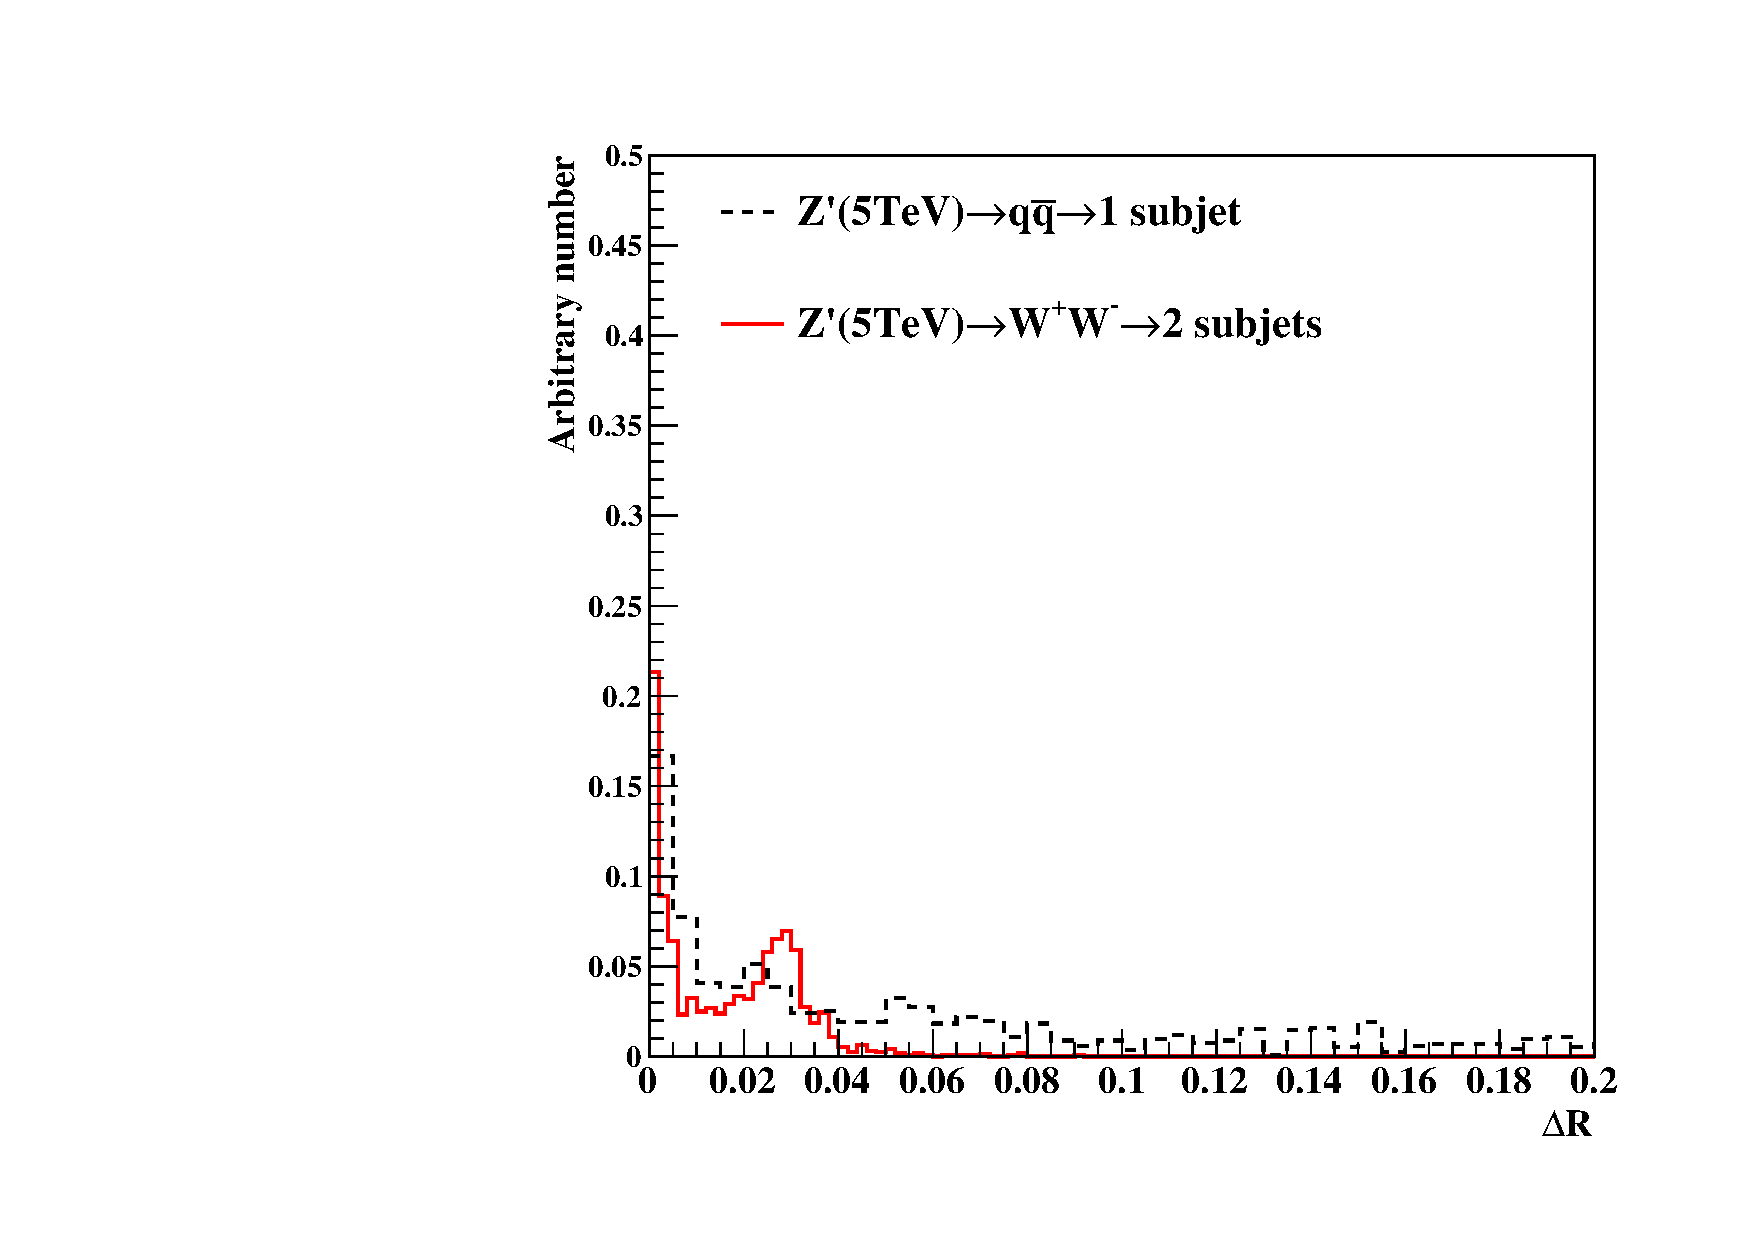
\includegraphics[width=0.3\textwidth]{/Users/ms08962476/Timing_paper/Pictures_used_for_FCC_and_jets/Truth_dR_Dis/5TeV/dR_T_3_5TeV_Truth.pdf}
   }
   \subfigure[The fifth trailing-T] {
   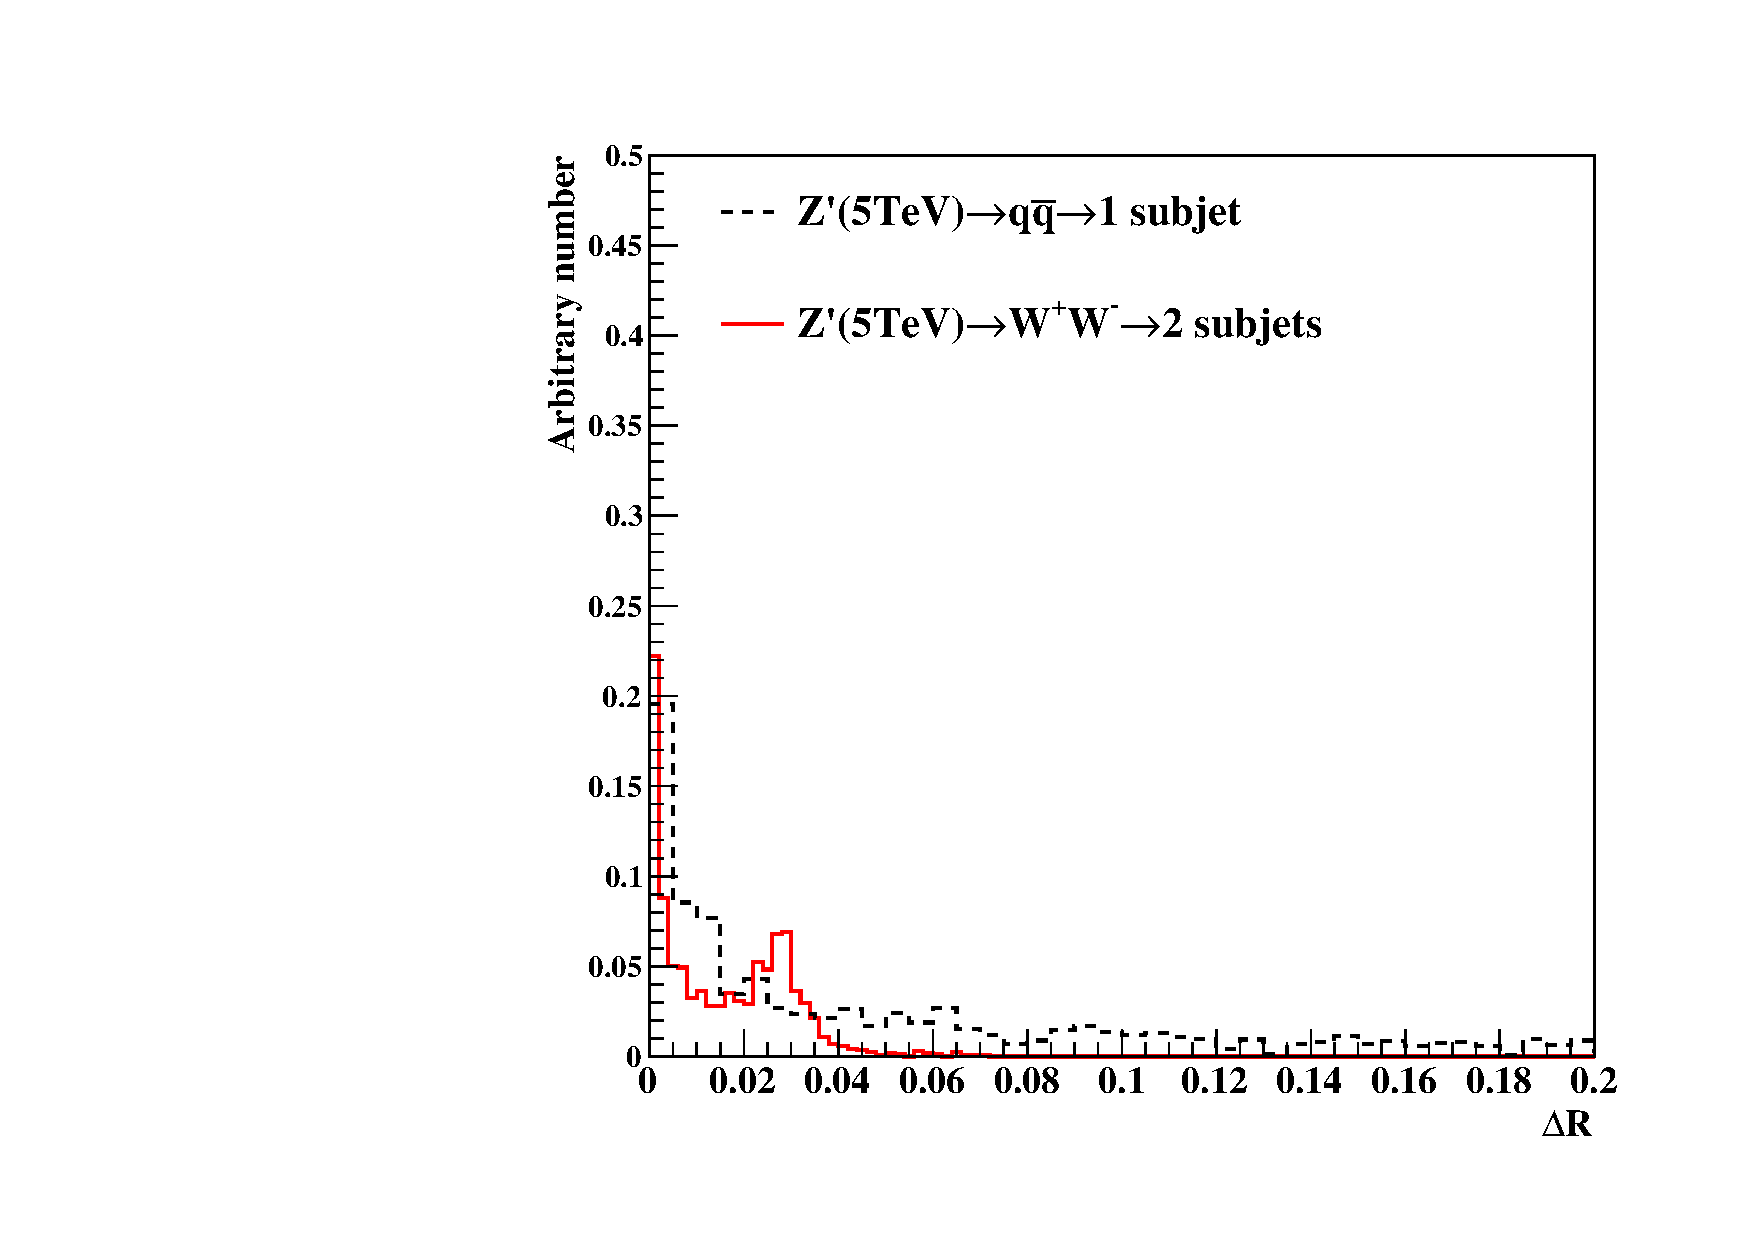
\includegraphics[width=0.3\textwidth]{/Users/ms08962476/Timing_paper/Pictures_used_for_FCC_and_jets/Truth_dR_Dis/5TeV/dR_T_4_5TeV_Truth.pdf}
   }
\end{center}
\caption{Distributions of $\Delta R$ for $M(Z') = 5$~TeV for five kinds of trailing-T particles with the truth-level information
are shown here. \label{fig:Truth_dR_Dis_5TeV_T}}
\end{figure}

\begin{figure}
\begin{center}
   \subfigure[The first trailing-$P_{T}$] {
   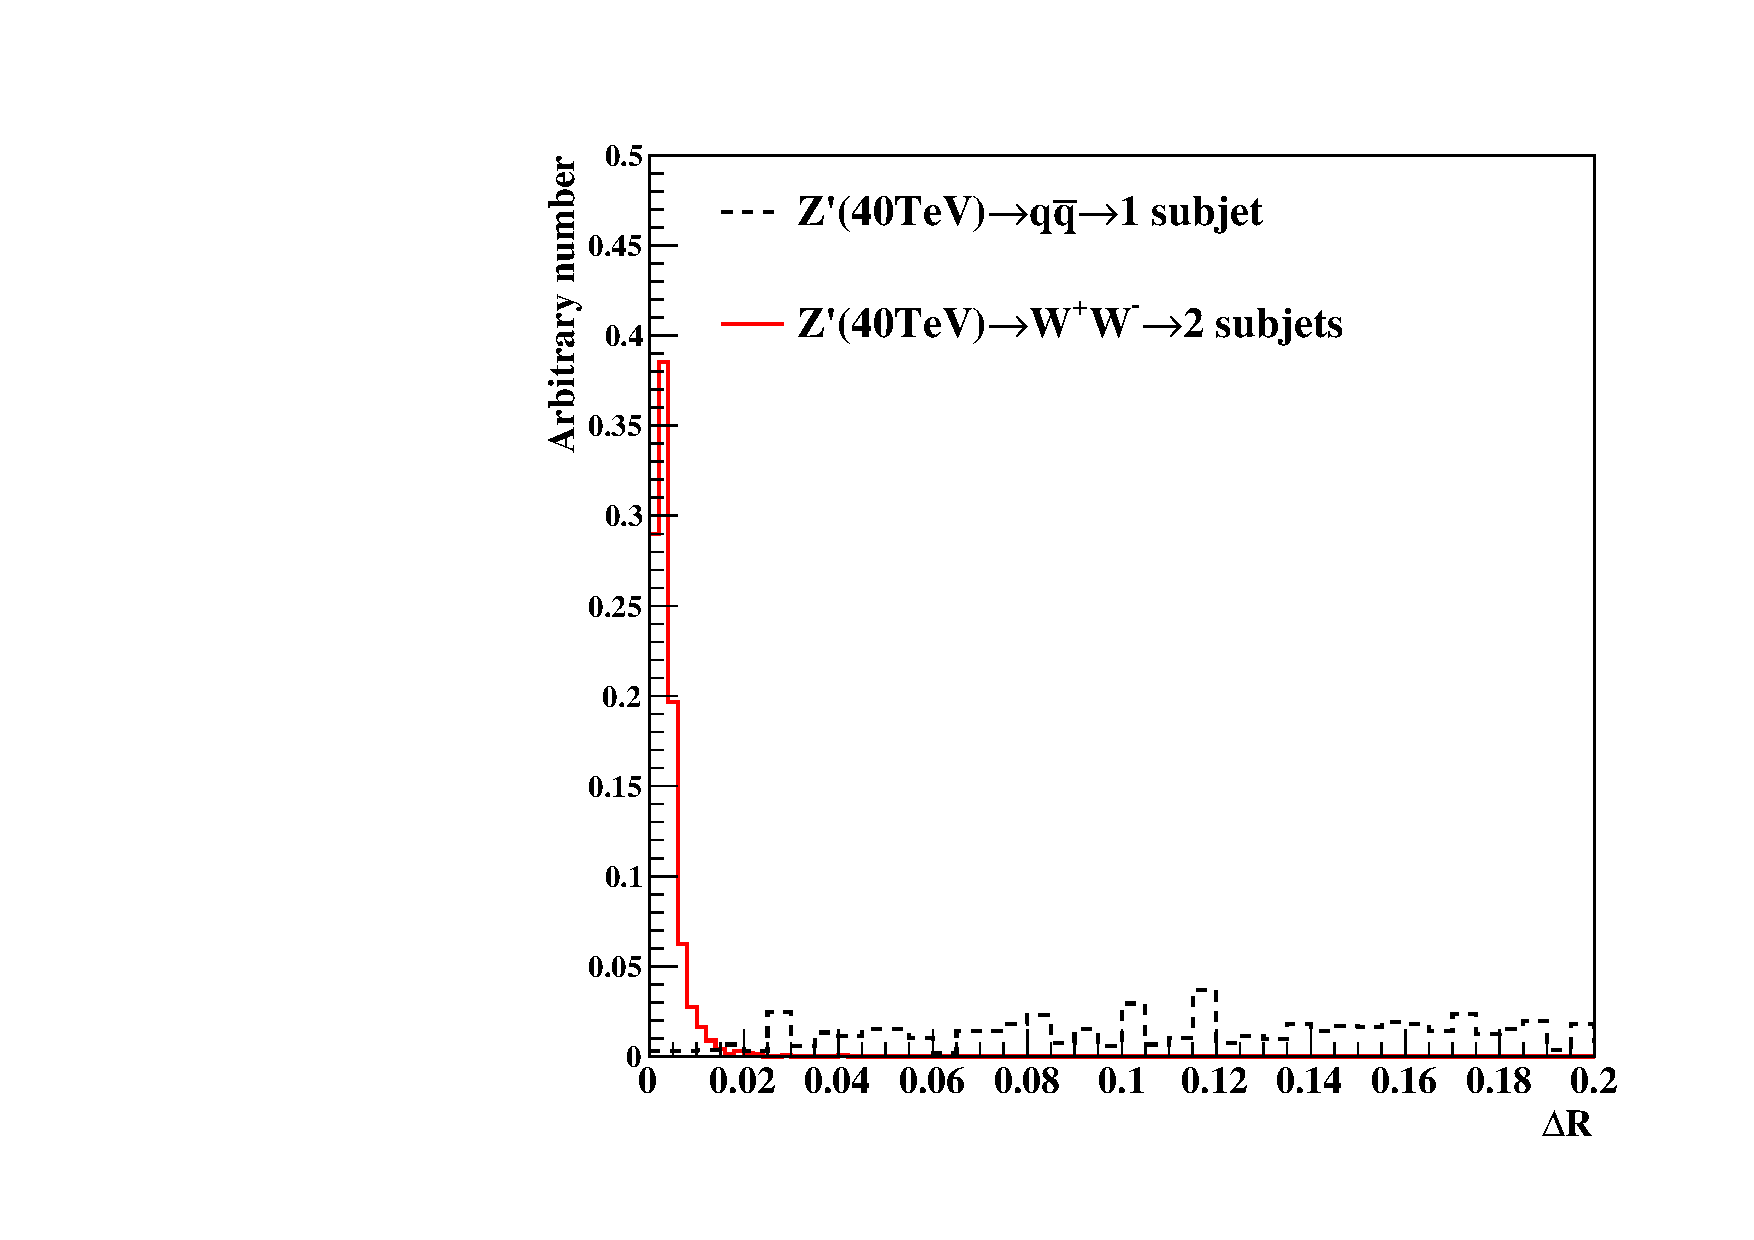
\includegraphics[width=0.3\textwidth]{/Users/ms08962476/Timing_paper/Pictures_used_for_FCC_and_jets/Truth_dR_Dis/40TeV/dR_PT_0_40TeV_Truth.pdf}
   }
   \subfigure[The second trailing-$P_{T}$] {
   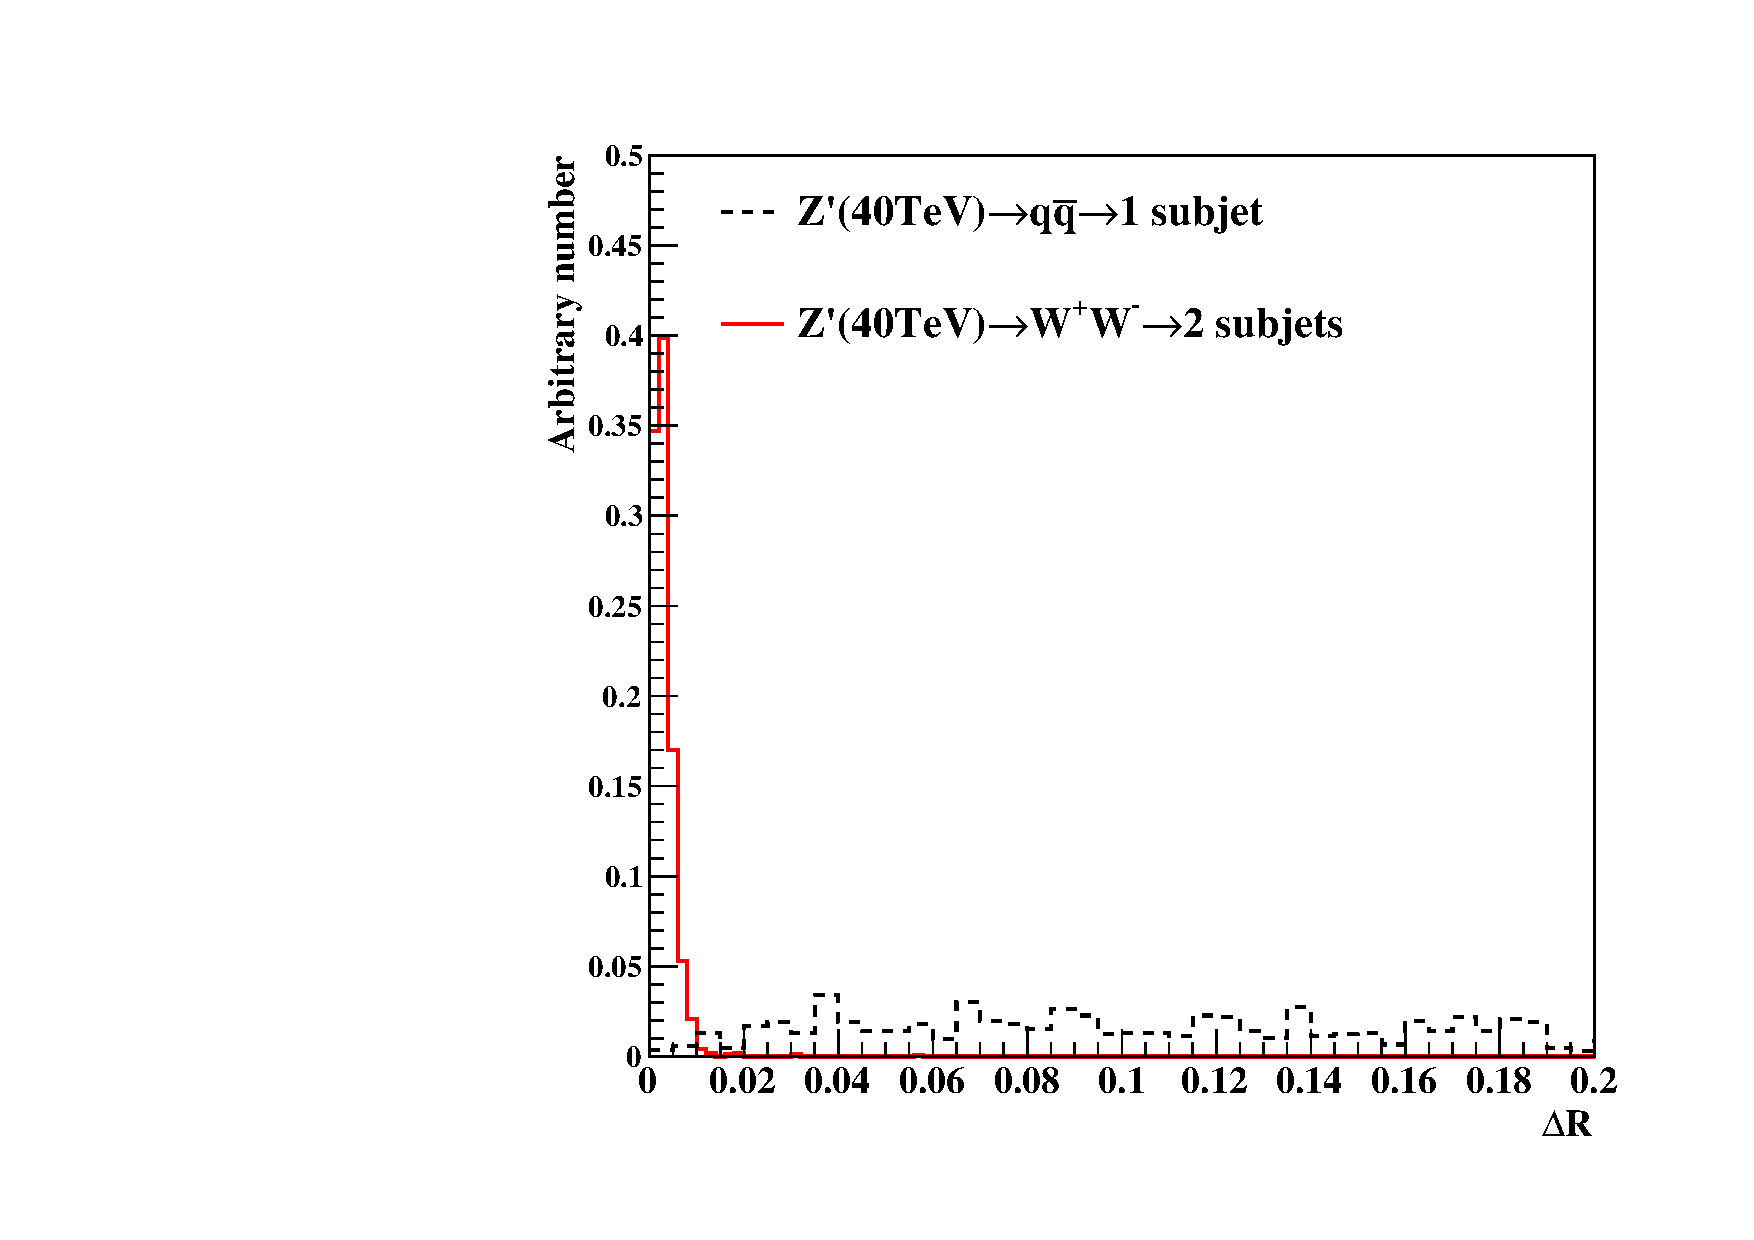
\includegraphics[width=0.3\textwidth]{/Users/ms08962476/Timing_paper/Pictures_used_for_FCC_and_jets/Truth_dR_Dis/40TeV/dR_PT_1_40TeV_Truth.pdf}
   }
   \subfigure[The third trailing-$P_{T}$] {
   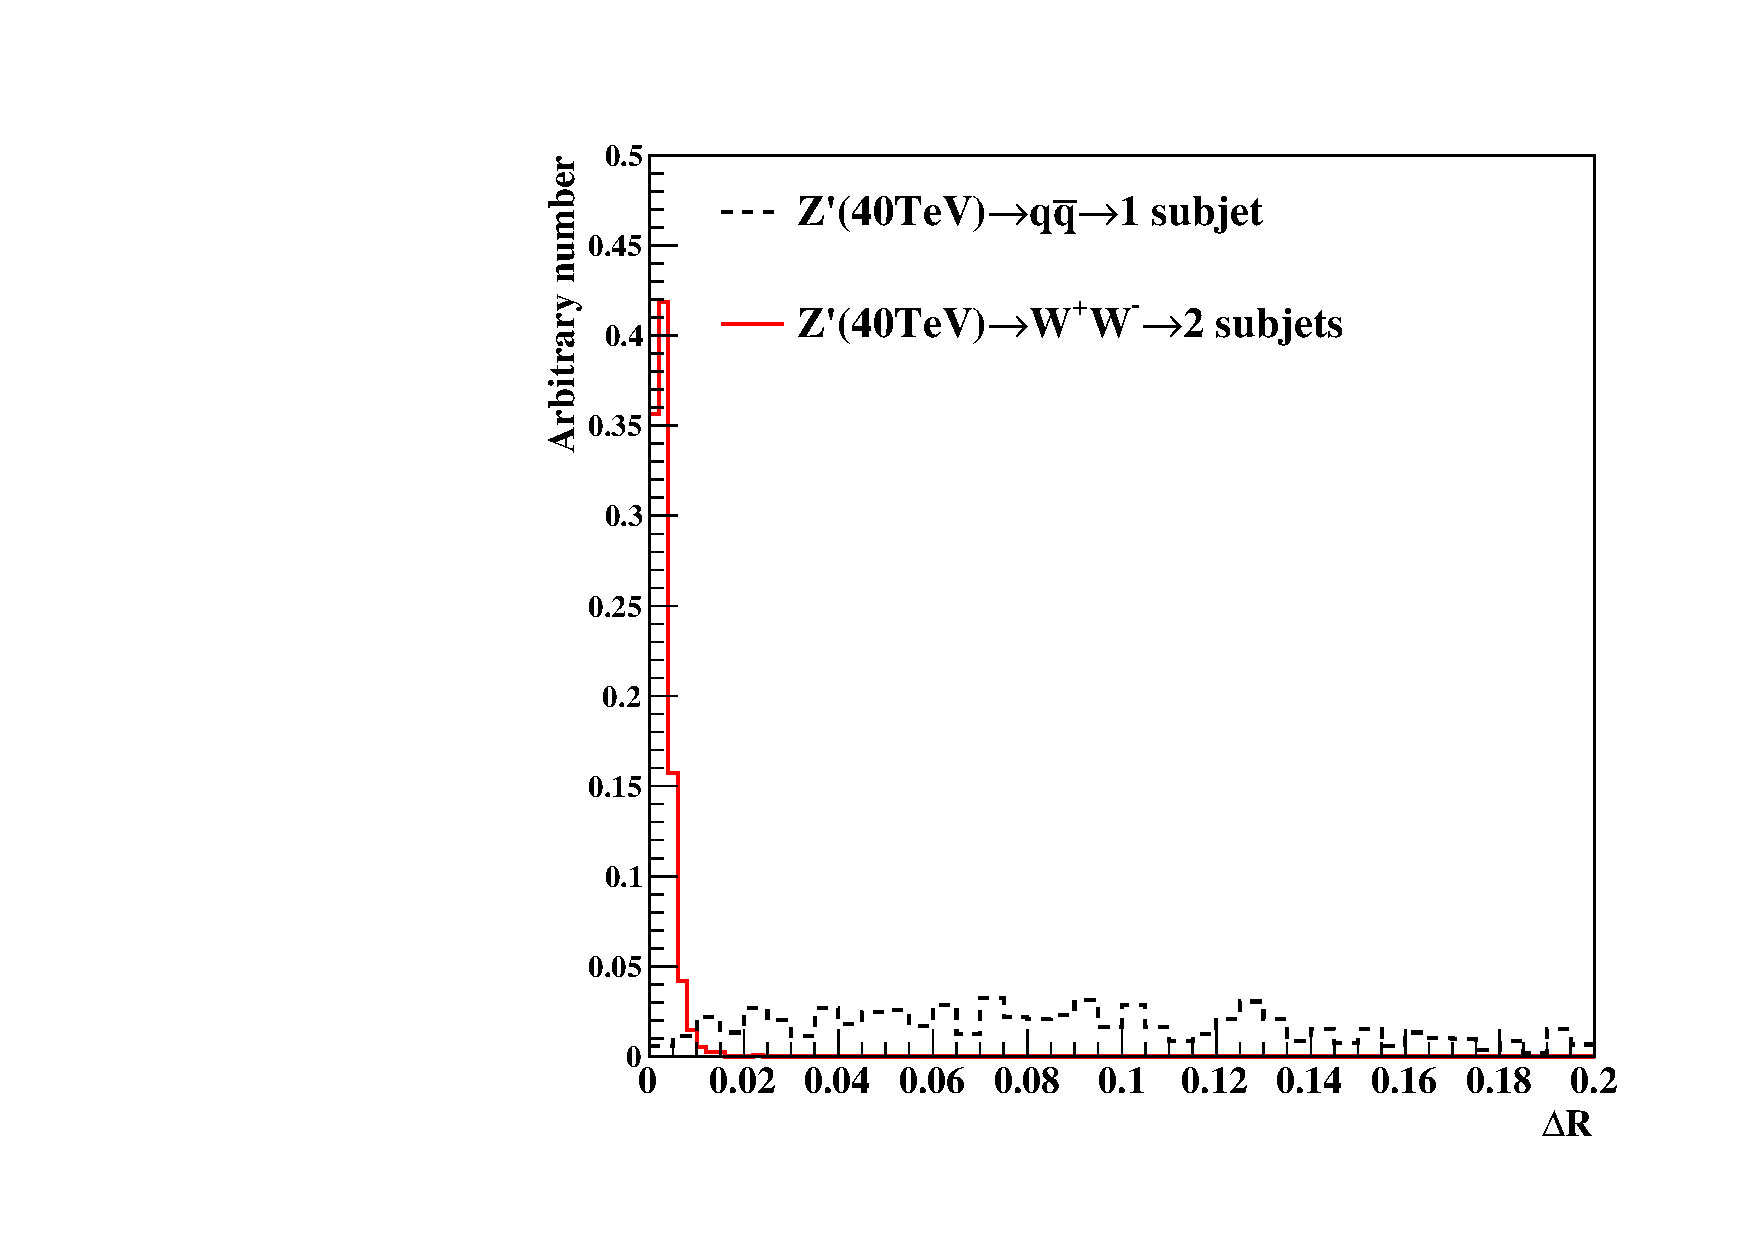
\includegraphics[width=0.3\textwidth]{/Users/ms08962476/Timing_paper/Pictures_used_for_FCC_and_jets/Truth_dR_Dis/40TeV/dR_PT_2_40TeV_Truth.pdf}
   }
   \subfigure[The fourth trailing-$P_{T}$] {
   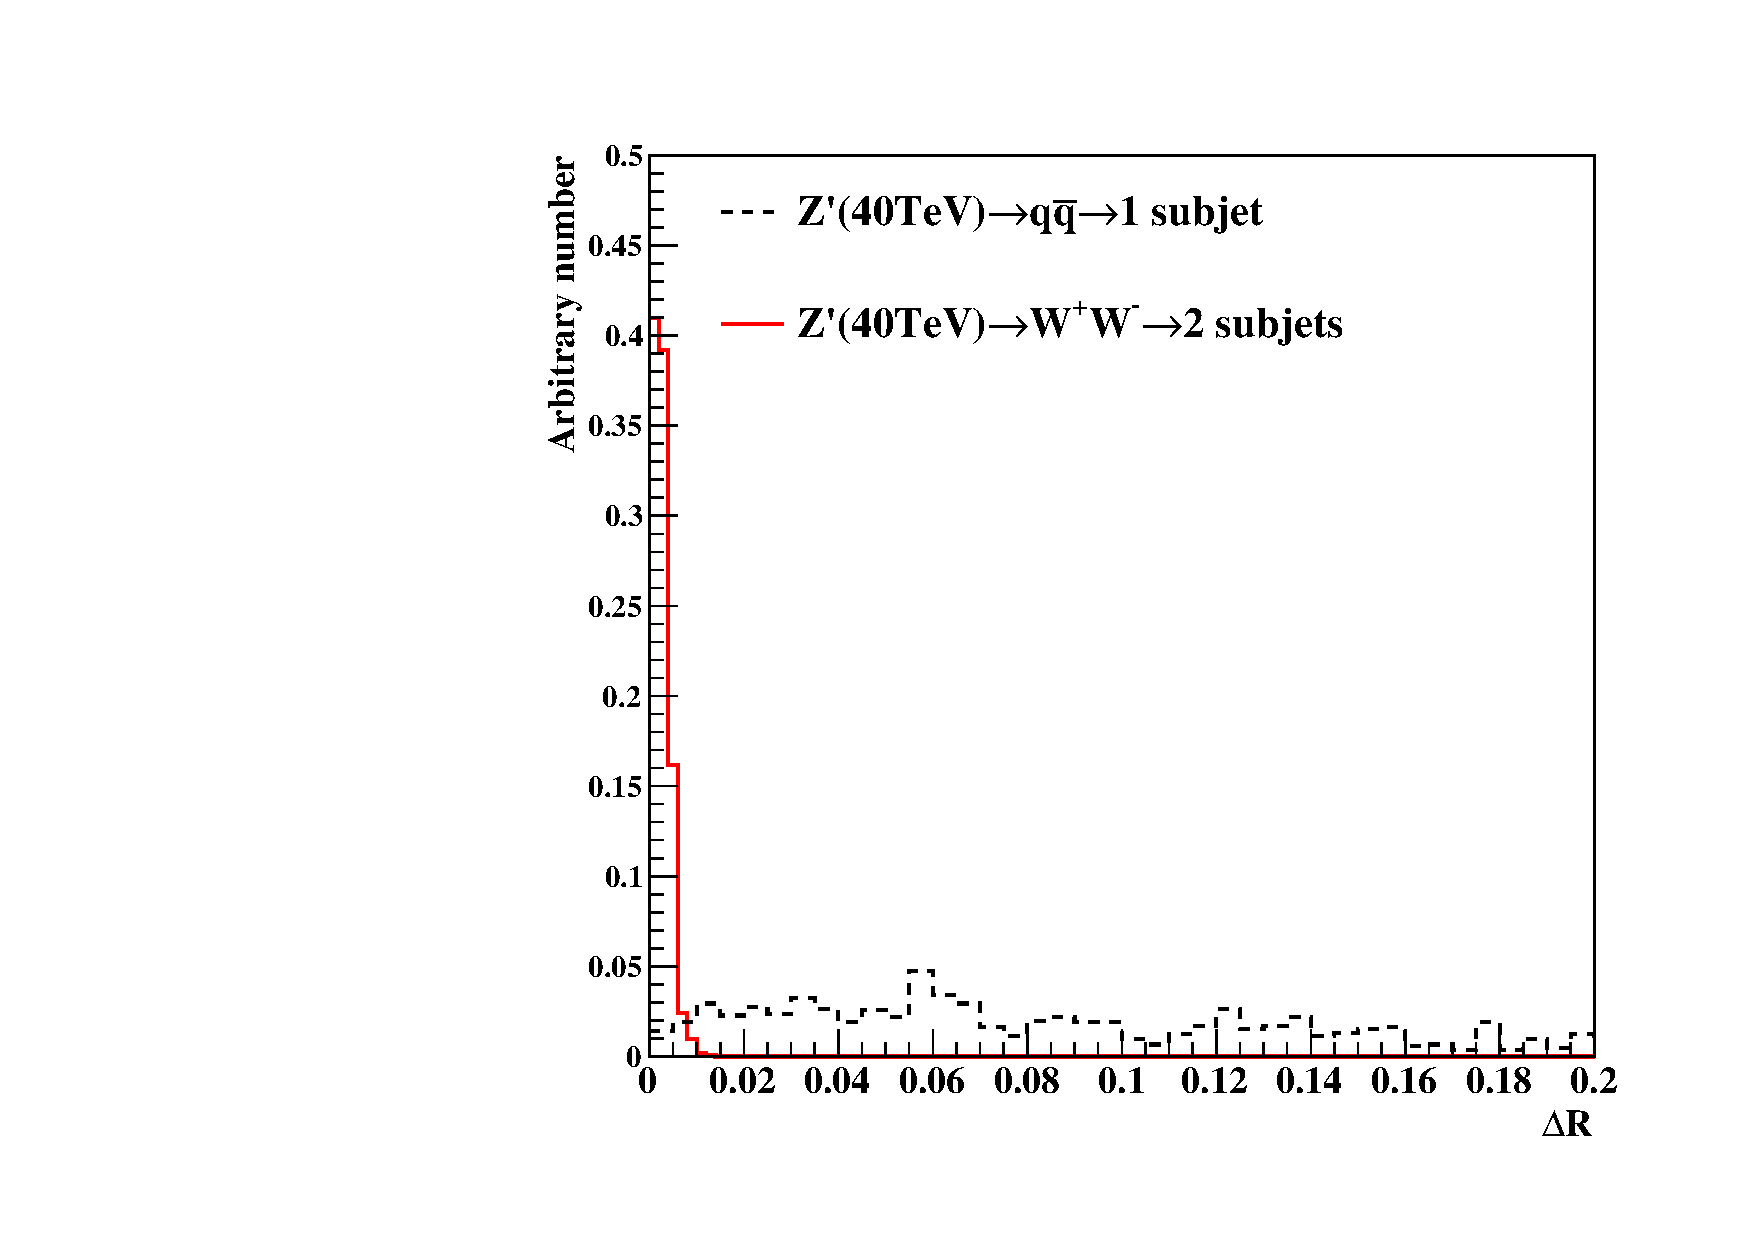
\includegraphics[width=0.3\textwidth]{/Users/ms08962476/Timing_paper/Pictures_used_for_FCC_and_jets/Truth_dR_Dis/40TeV/dR_PT_3_40TeV_Truth.pdf}
   }
   \subfigure[The fifth trailing-$P_{T}$] {
   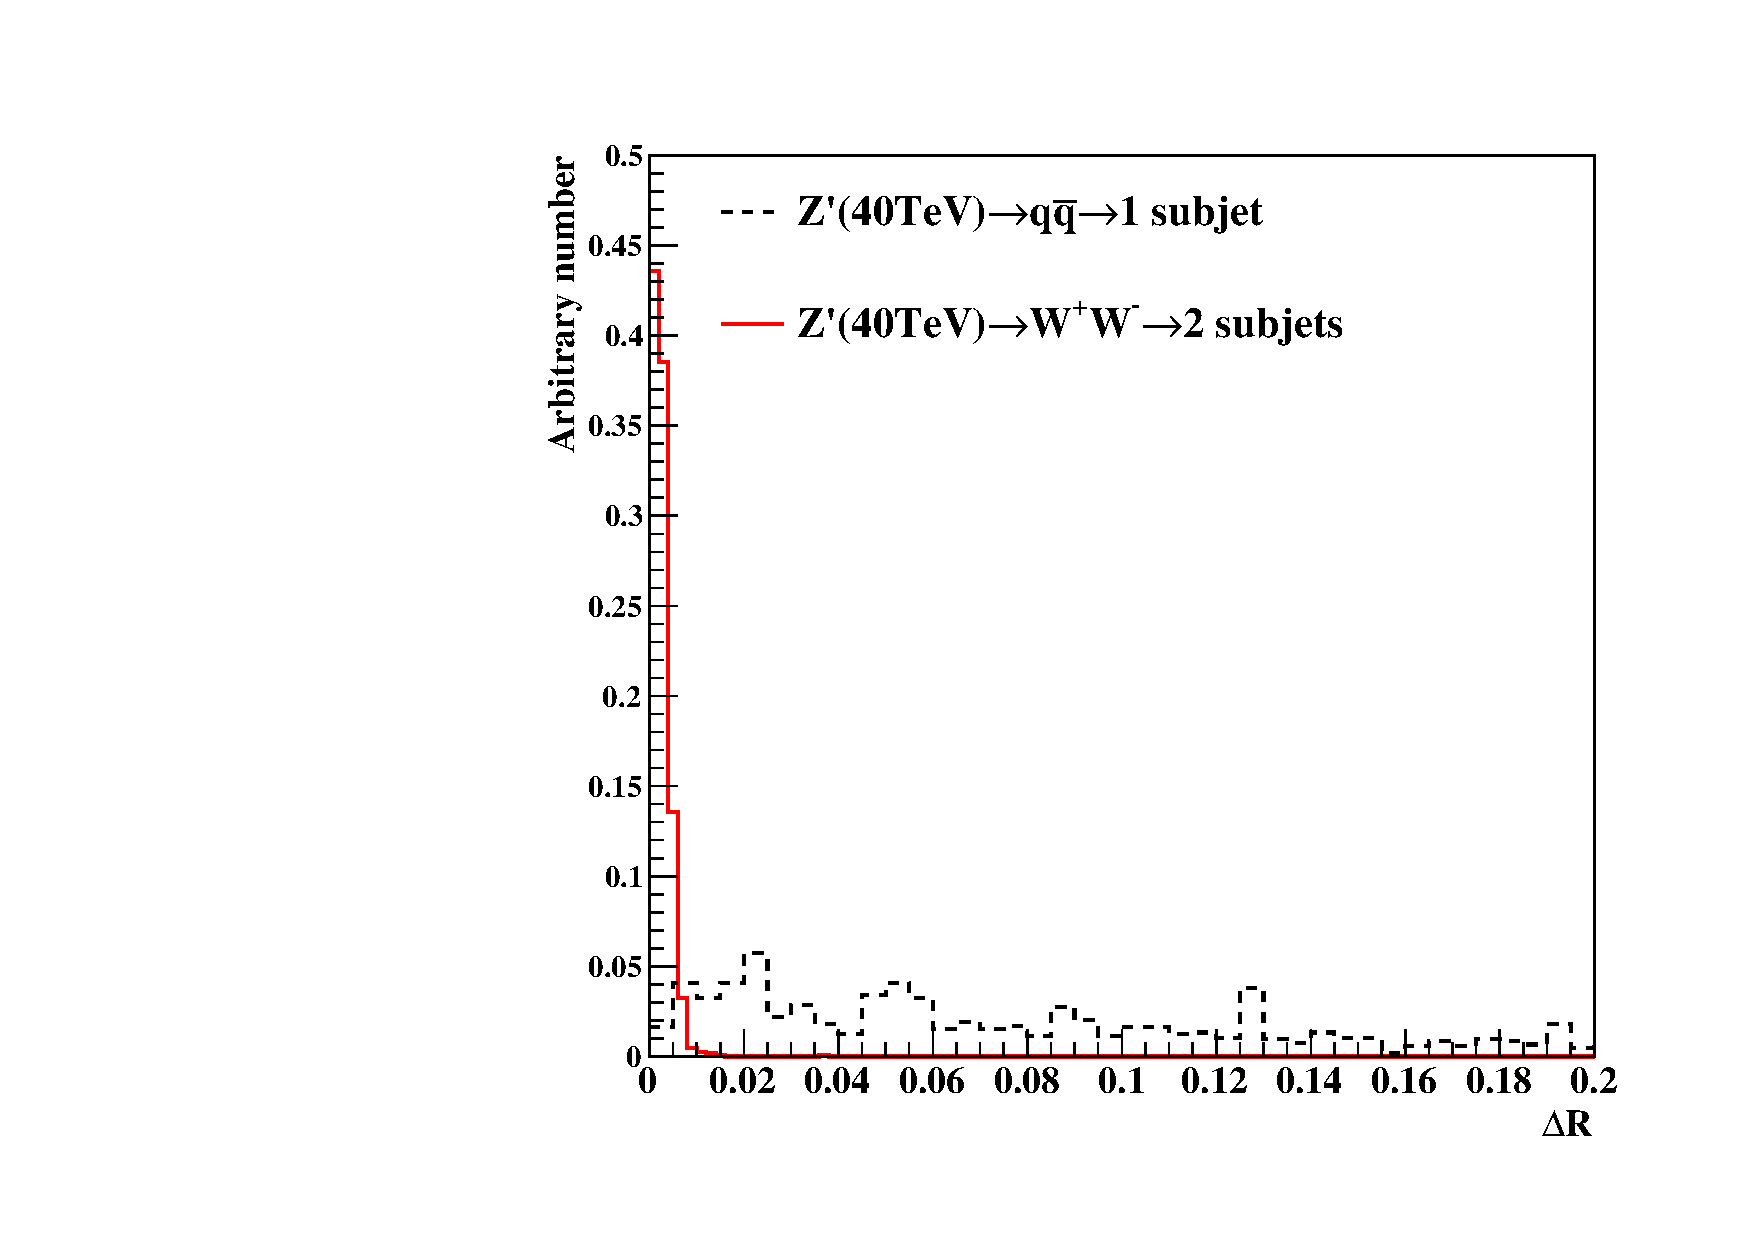
\includegraphics[width=0.3\textwidth]{/Users/ms08962476/Timing_paper/Pictures_used_for_FCC_and_jets/Truth_dR_Dis/40TeV/dR_PT_4_40TeV_Truth.pdf}
   }
\end{center}
\caption{Distributions of $\Delta R$ for $M(Z') = 40$~TeV for five kinds of trailing-$P_{T}$ particles with the truth-level information
are shown here. \label{fig:Truth_dR_Dis_40TeV_PT}}
\end{figure}

\begin{figure}
\begin{center}
   \subfigure[The first trailing-T] {
   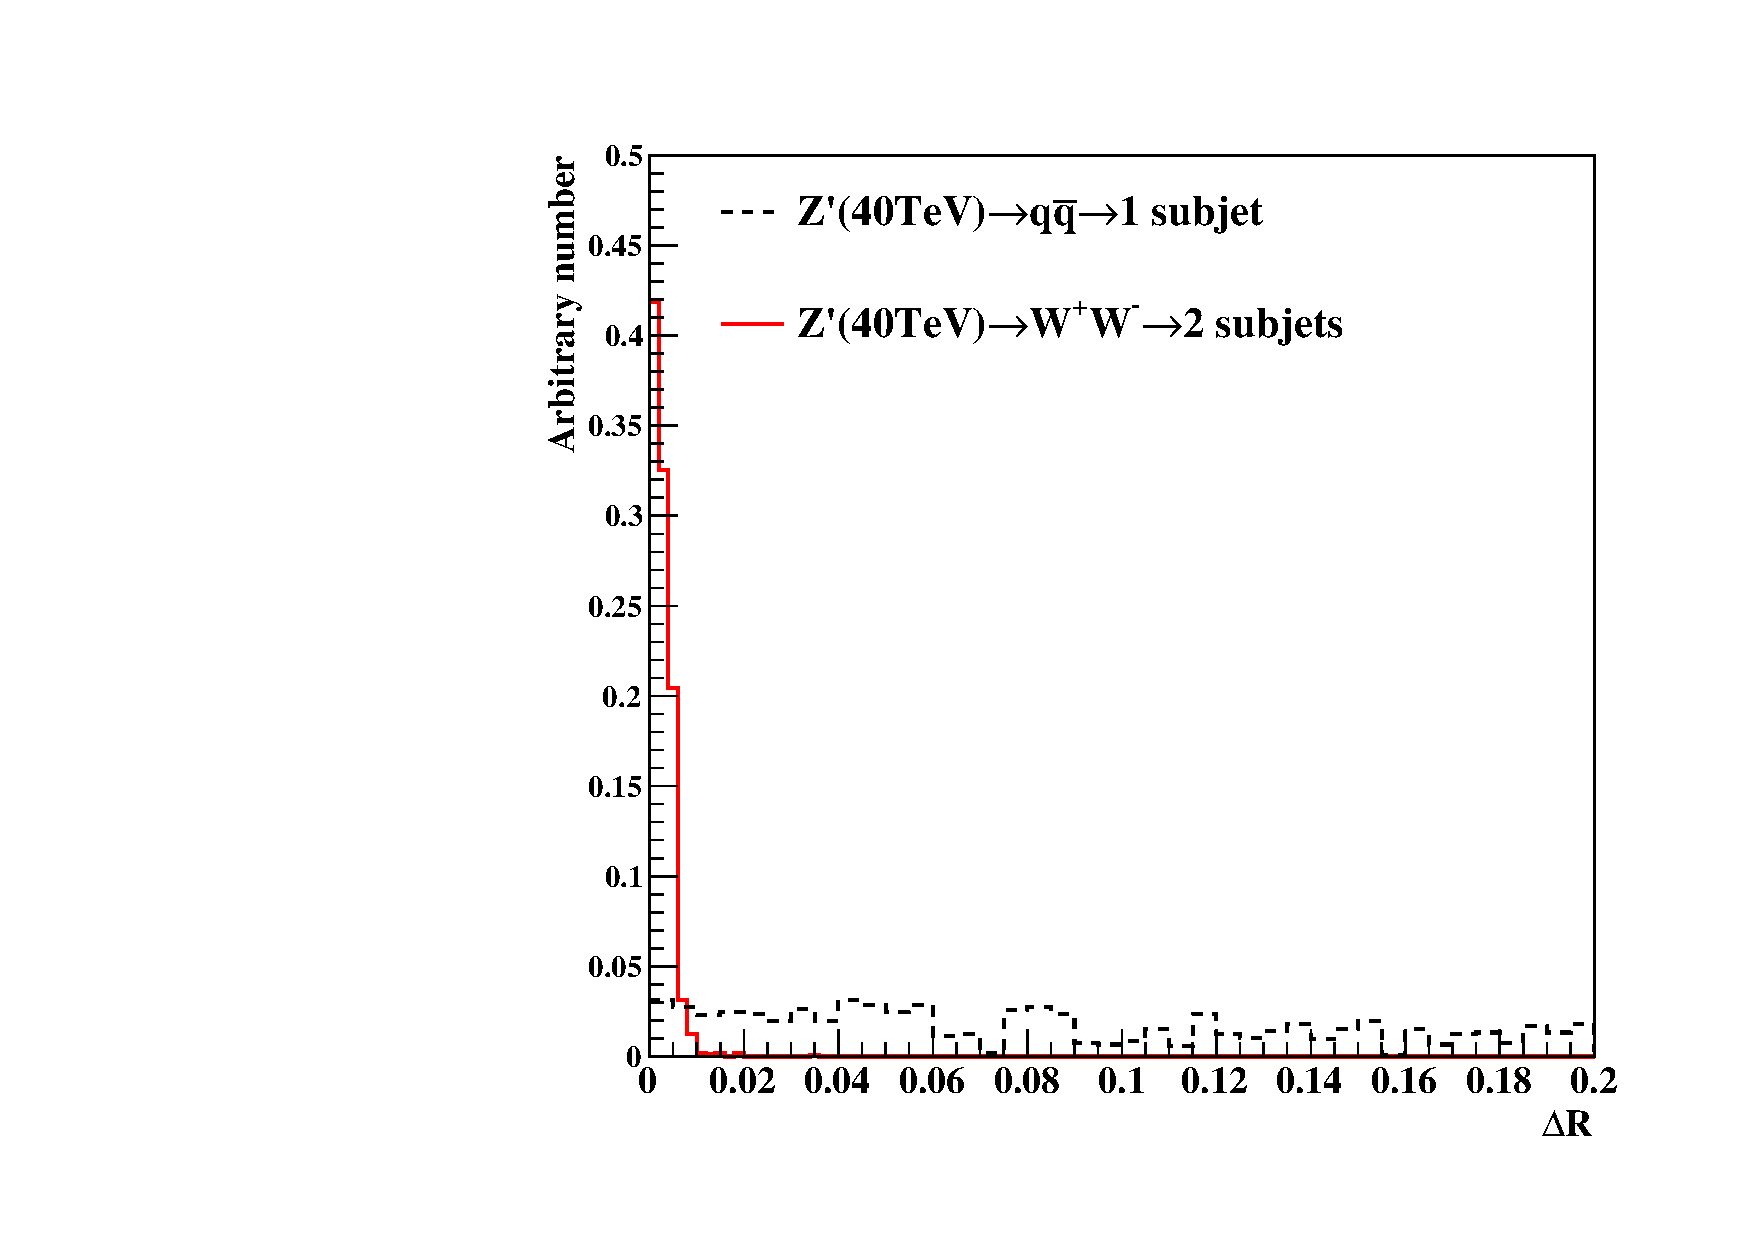
\includegraphics[width=0.3\textwidth]{/Users/ms08962476/Timing_paper/Pictures_used_for_FCC_and_jets/Truth_dR_Dis/40TeV/dR_T_0_40TeV_Truth.pdf}
   }
   \subfigure[The second trailing-T] {
   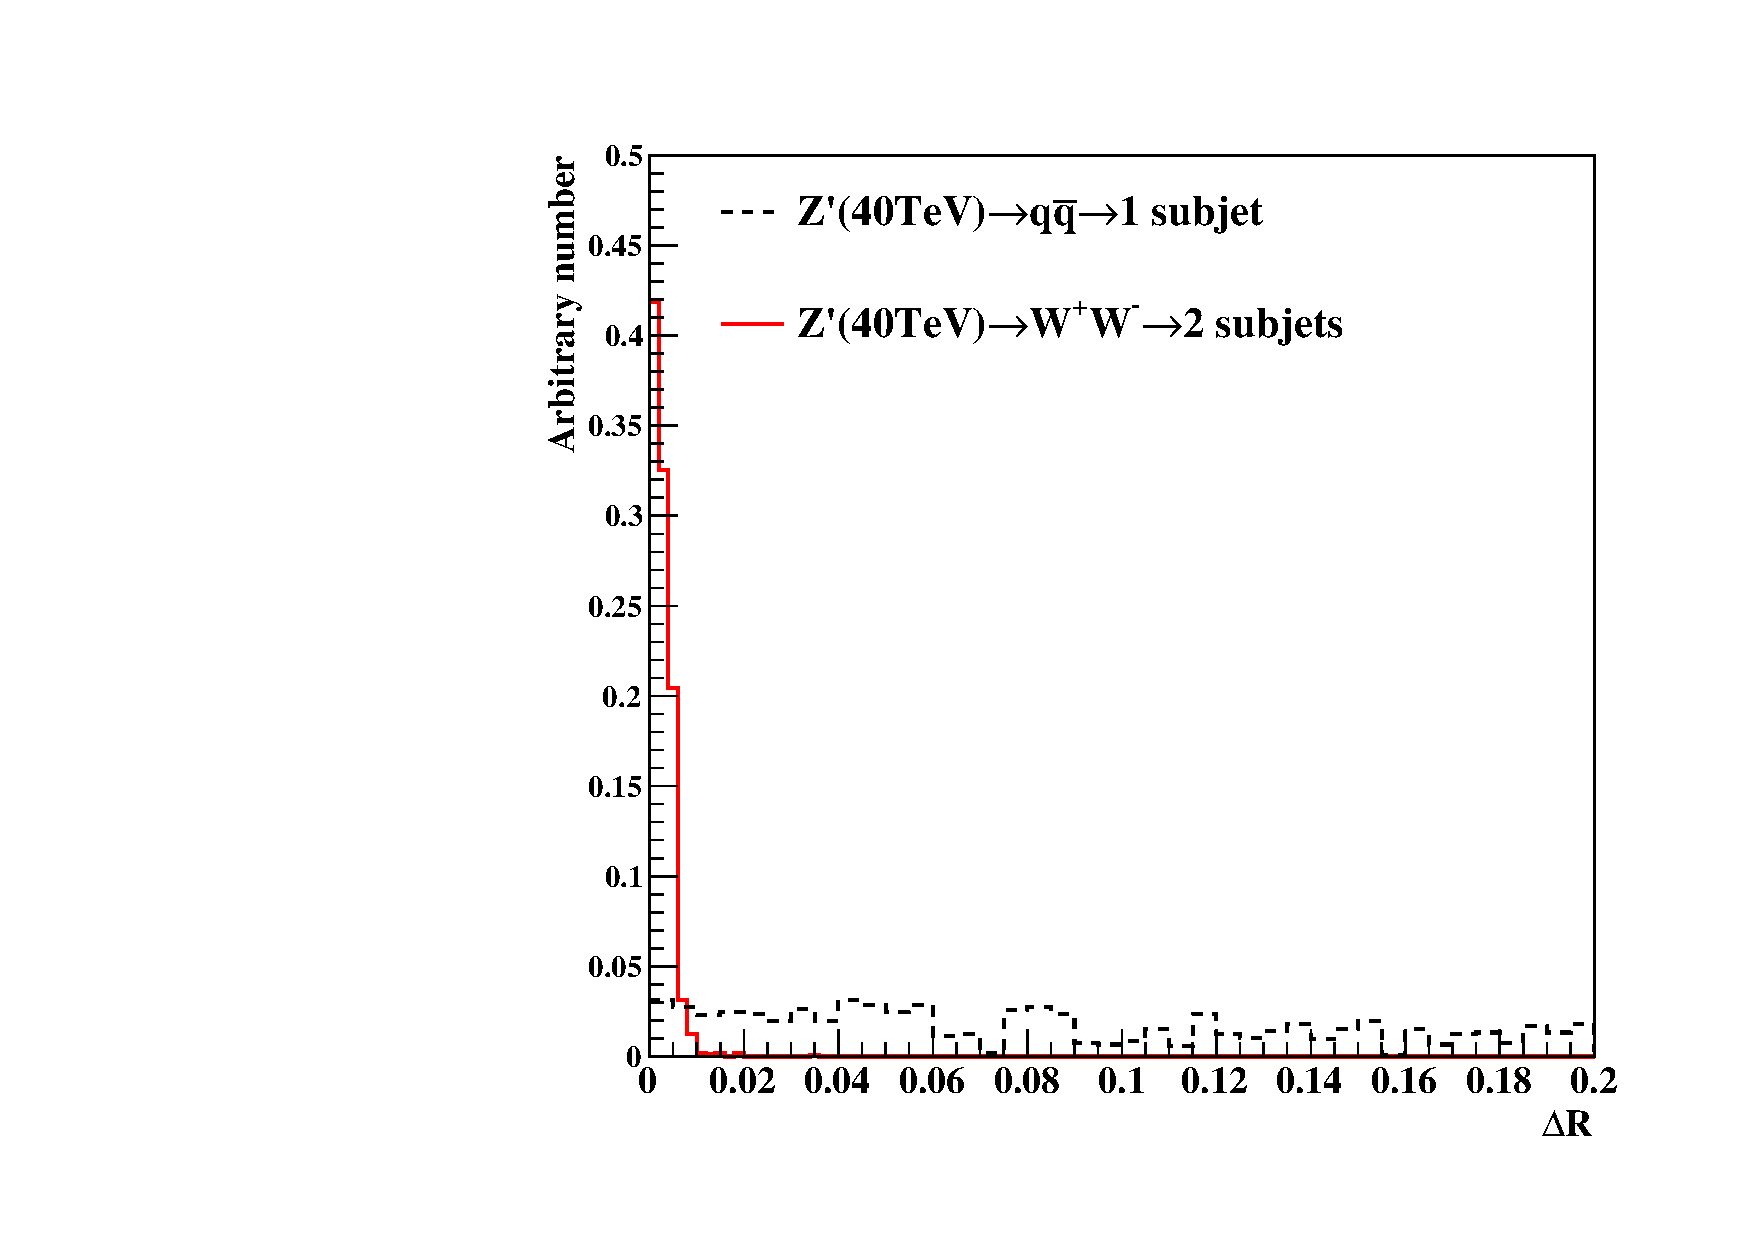
\includegraphics[width=0.3\textwidth]{/Users/ms08962476/Timing_paper/Pictures_used_for_FCC_and_jets/Truth_dR_Dis/40TeV/dR_T_1_40TeV_Truth.pdf}
   }
   \subfigure[The third trailing-T] {
   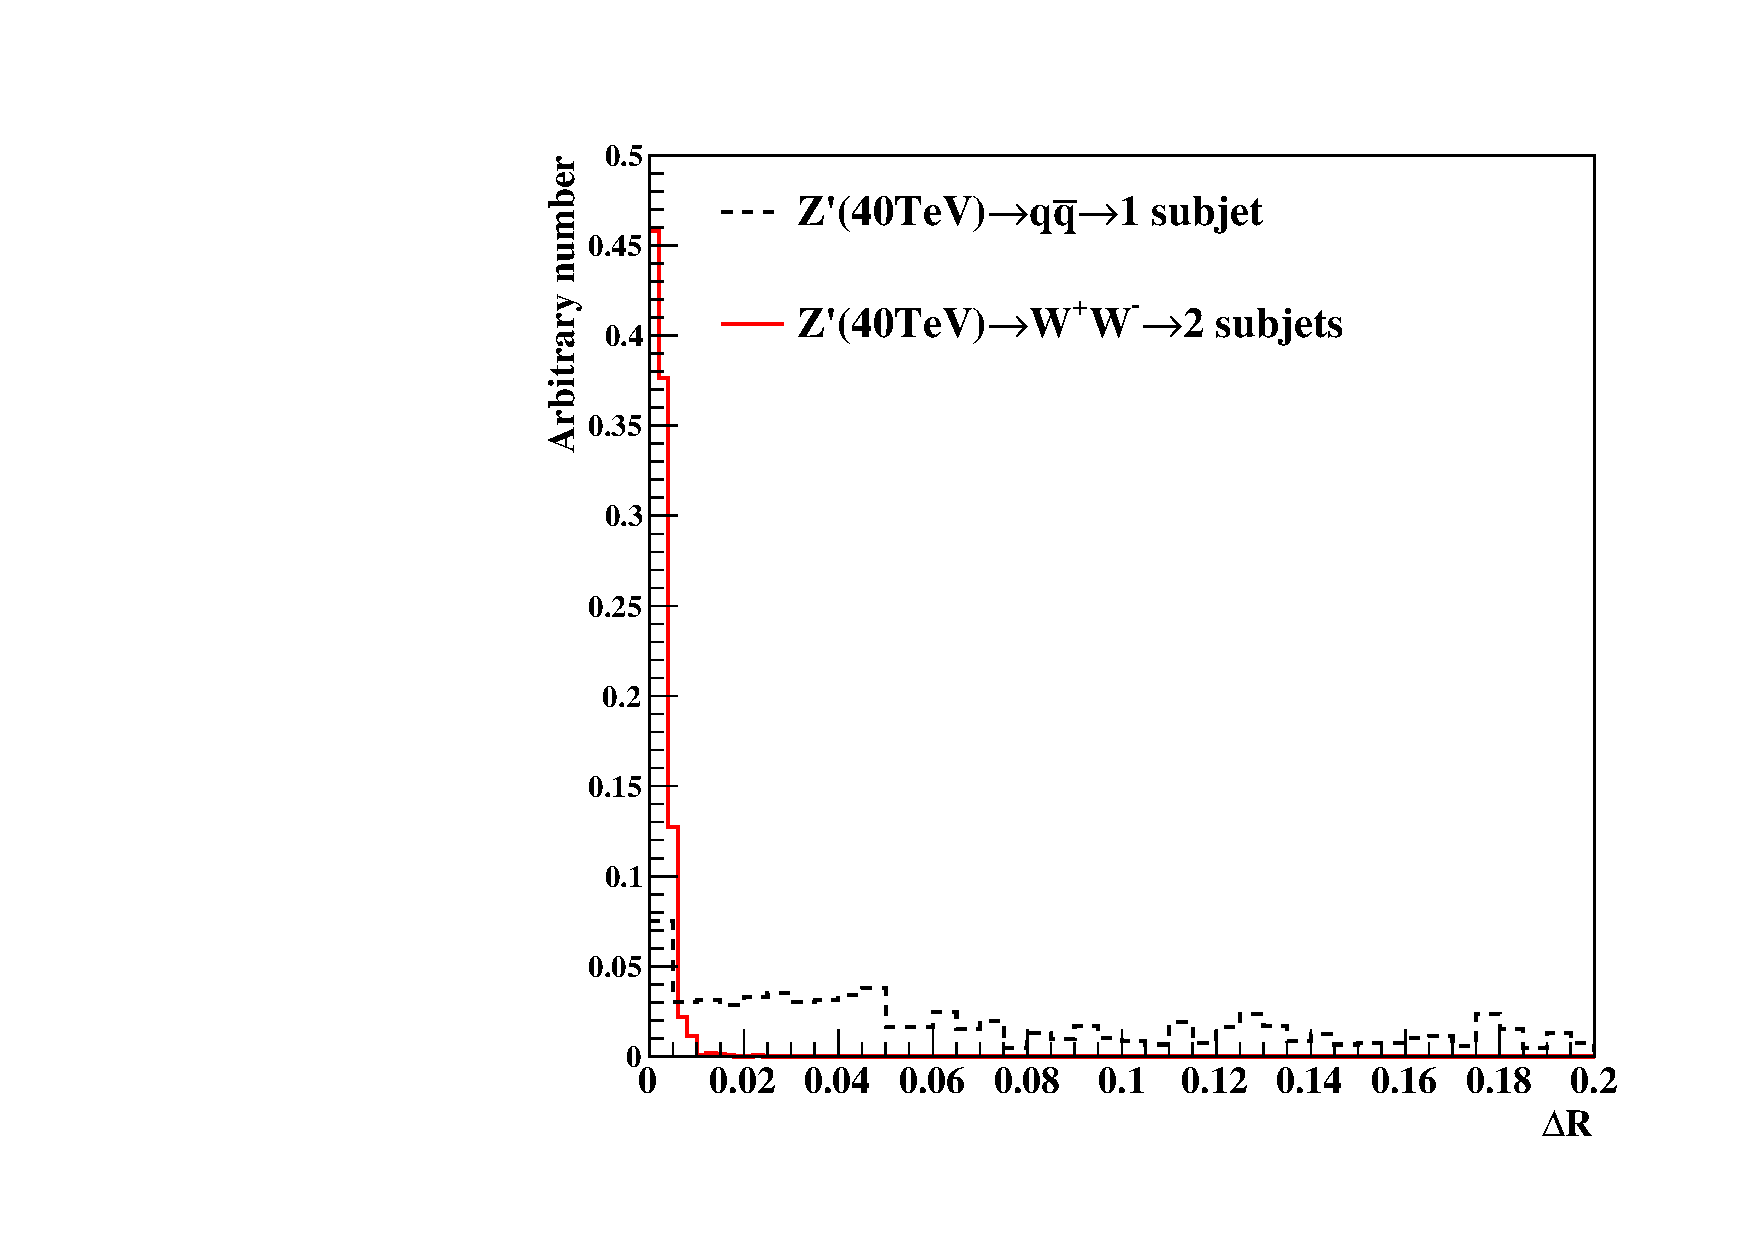
\includegraphics[width=0.3\textwidth]{/Users/ms08962476/Timing_paper/Pictures_used_for_FCC_and_jets/Truth_dR_Dis/40TeV/dR_T_2_40TeV_Truth.pdf}
   }
      \subfigure[The fourth trailing-T] {
   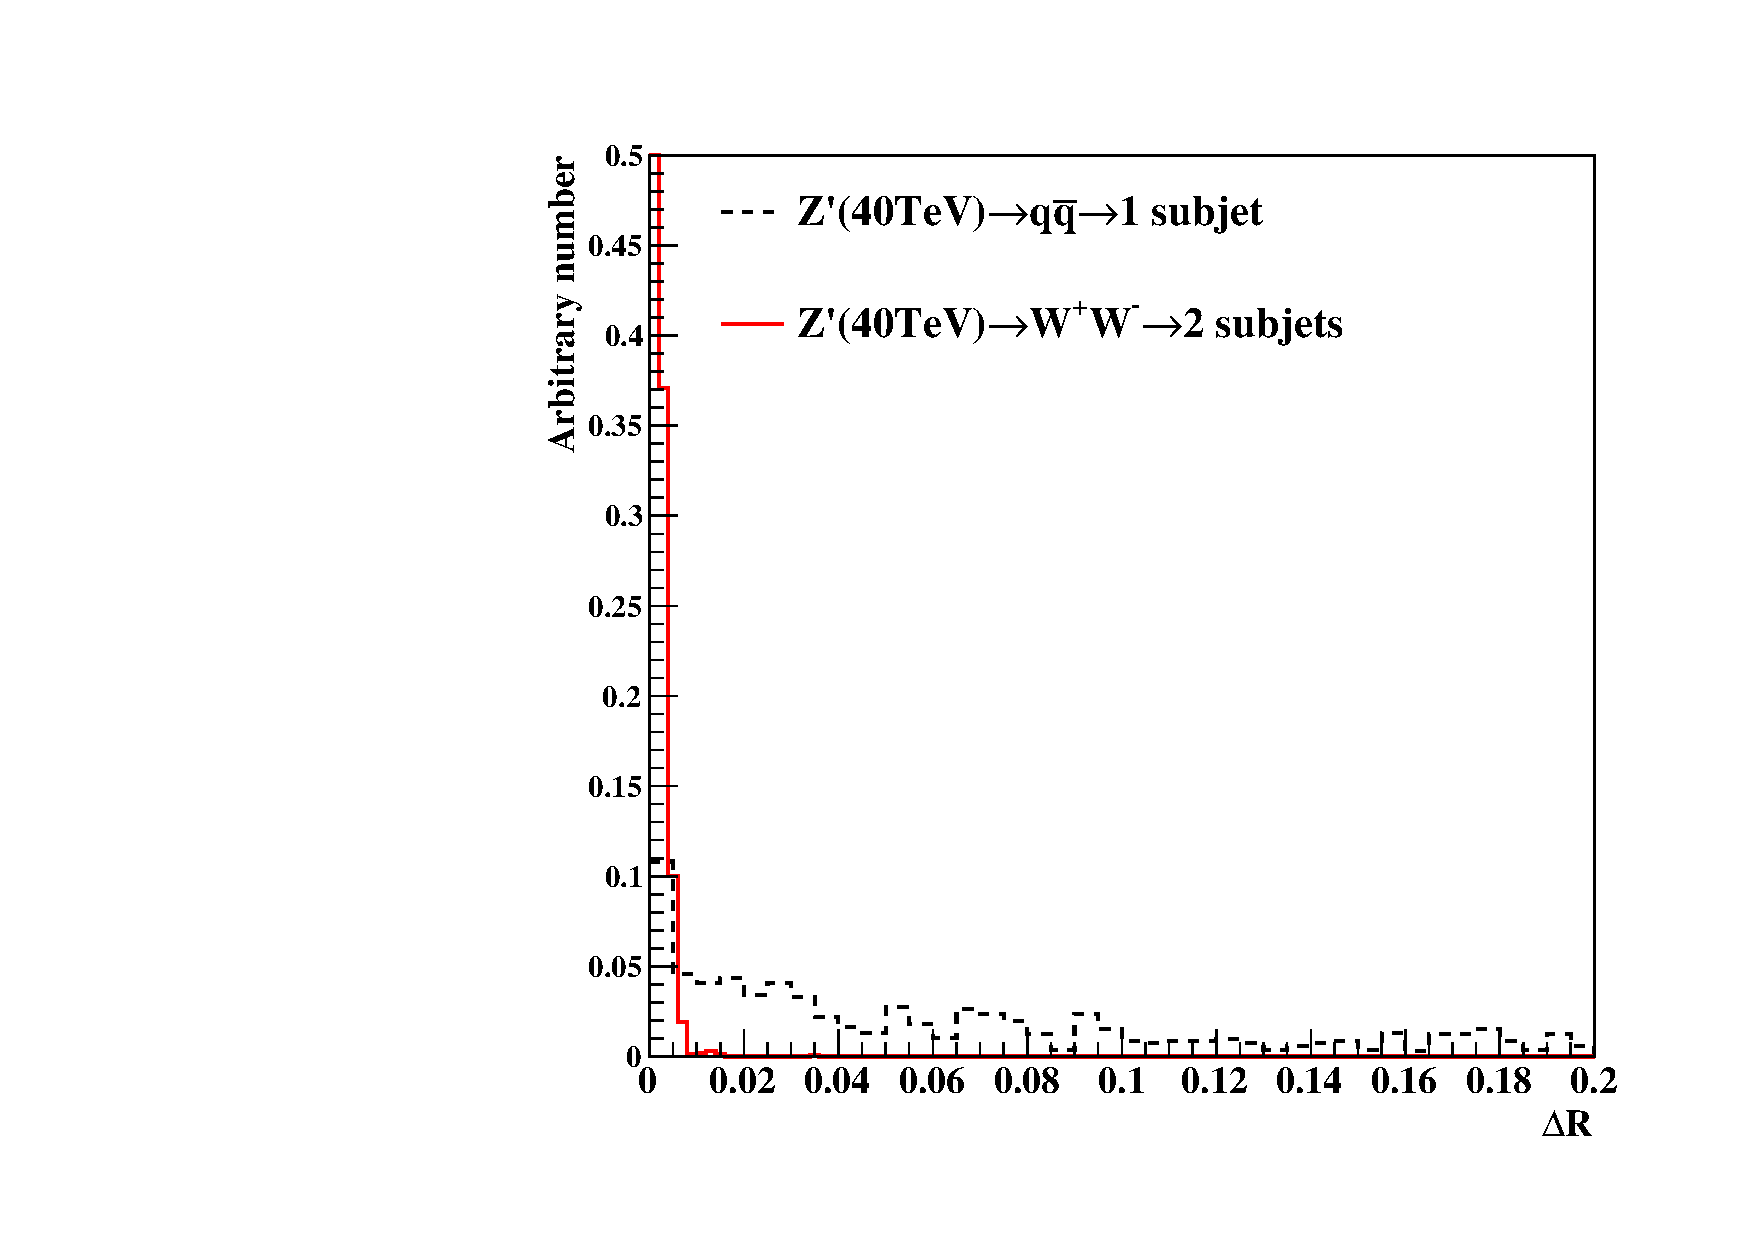
\includegraphics[width=0.3\textwidth]{/Users/ms08962476/Timing_paper/Pictures_used_for_FCC_and_jets/Truth_dR_Dis/40TeV/dR_T_3_40TeV_Truth.pdf}
   }
   \subfigure[The fifth trailing-$P_{T}$] {
   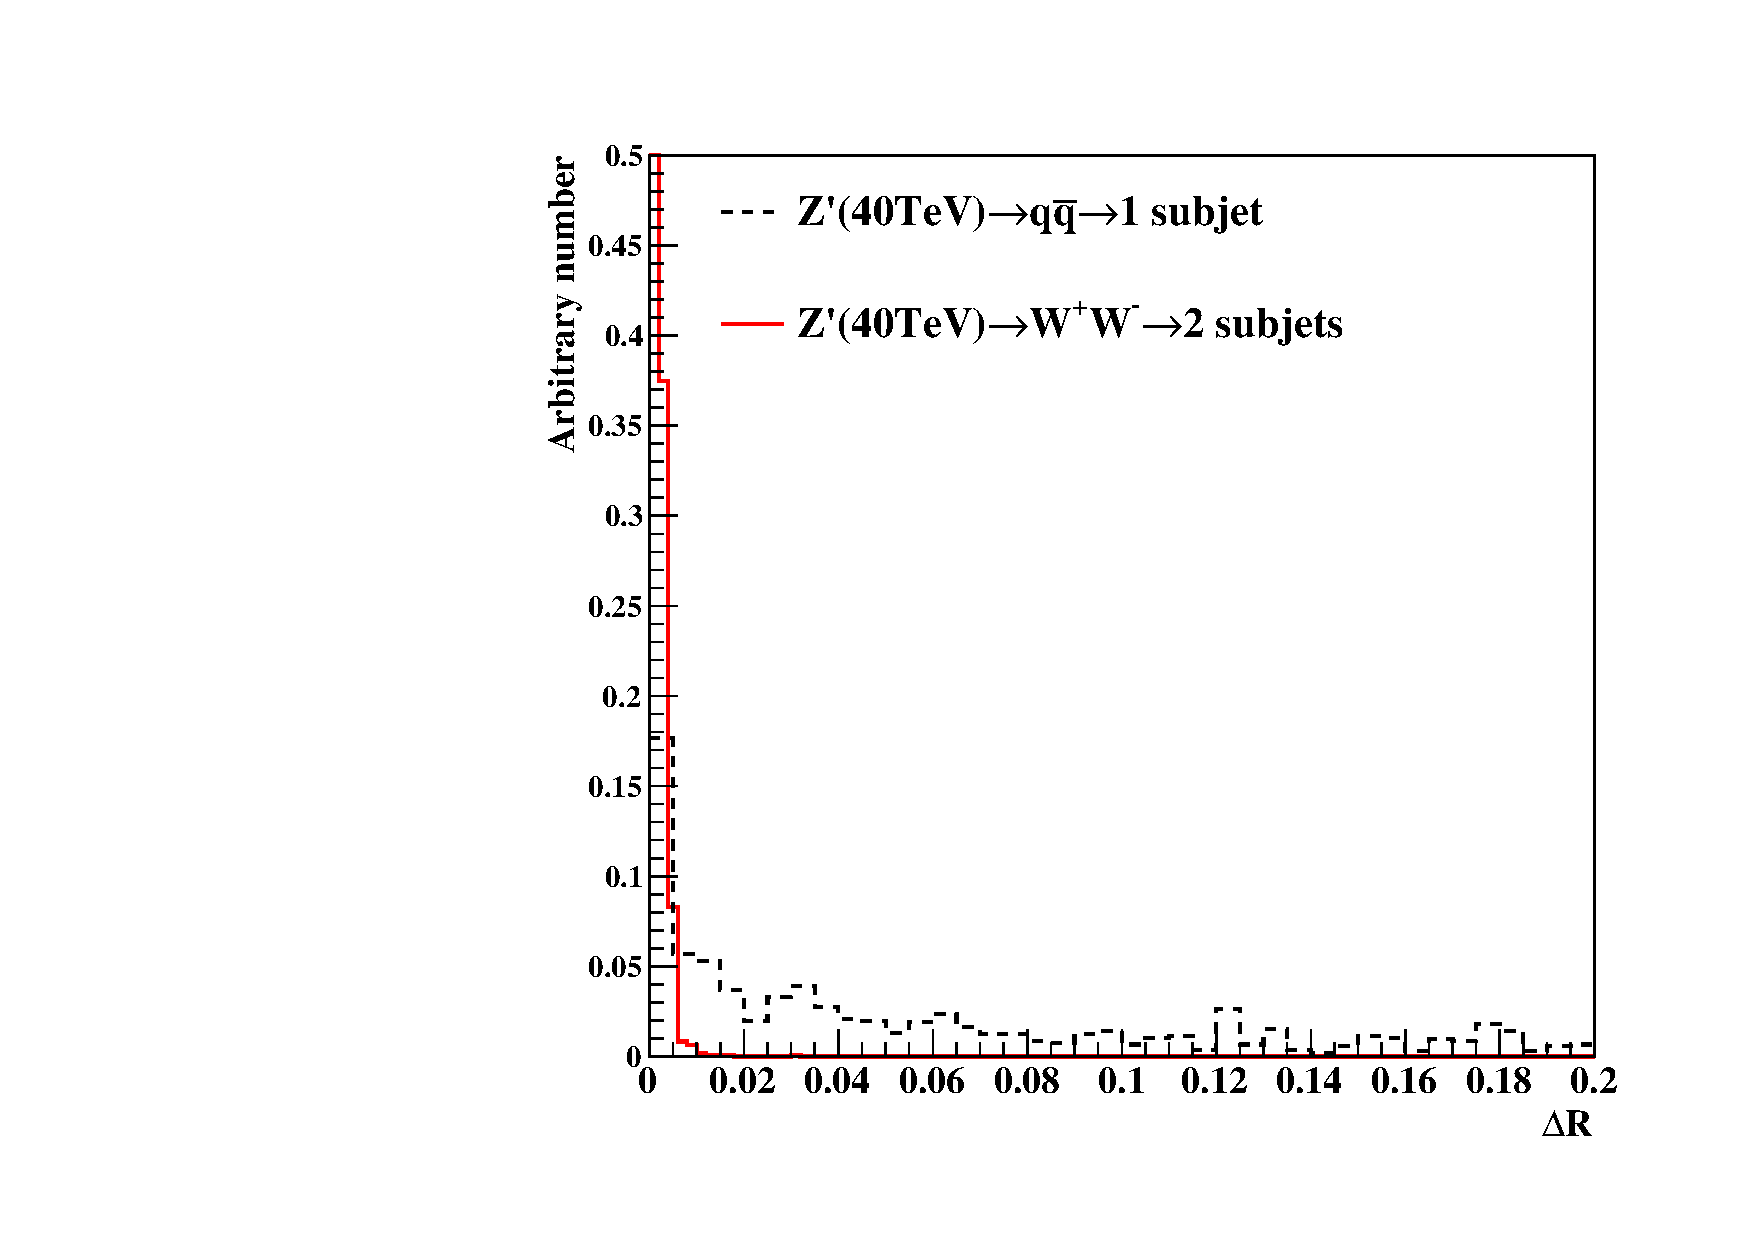
\includegraphics[width=0.3\textwidth]{/Users/ms08962476/Timing_paper/Pictures_used_for_FCC_and_jets/Truth_dR_Dis/40TeV/dR_T_4_40TeV_Truth.pdf}
   }
\end{center}
\caption{Distributions of $\Delta R$ for $M(Z') = 40$~TeV for five kinds of trailing-T particles with the true information
are shown here. \label{fig:Truth_dR_Dis_40TeV_T}}
\end{figure}

\begin{figure}
\begin{center}
   \subfigure[5TeV] {
   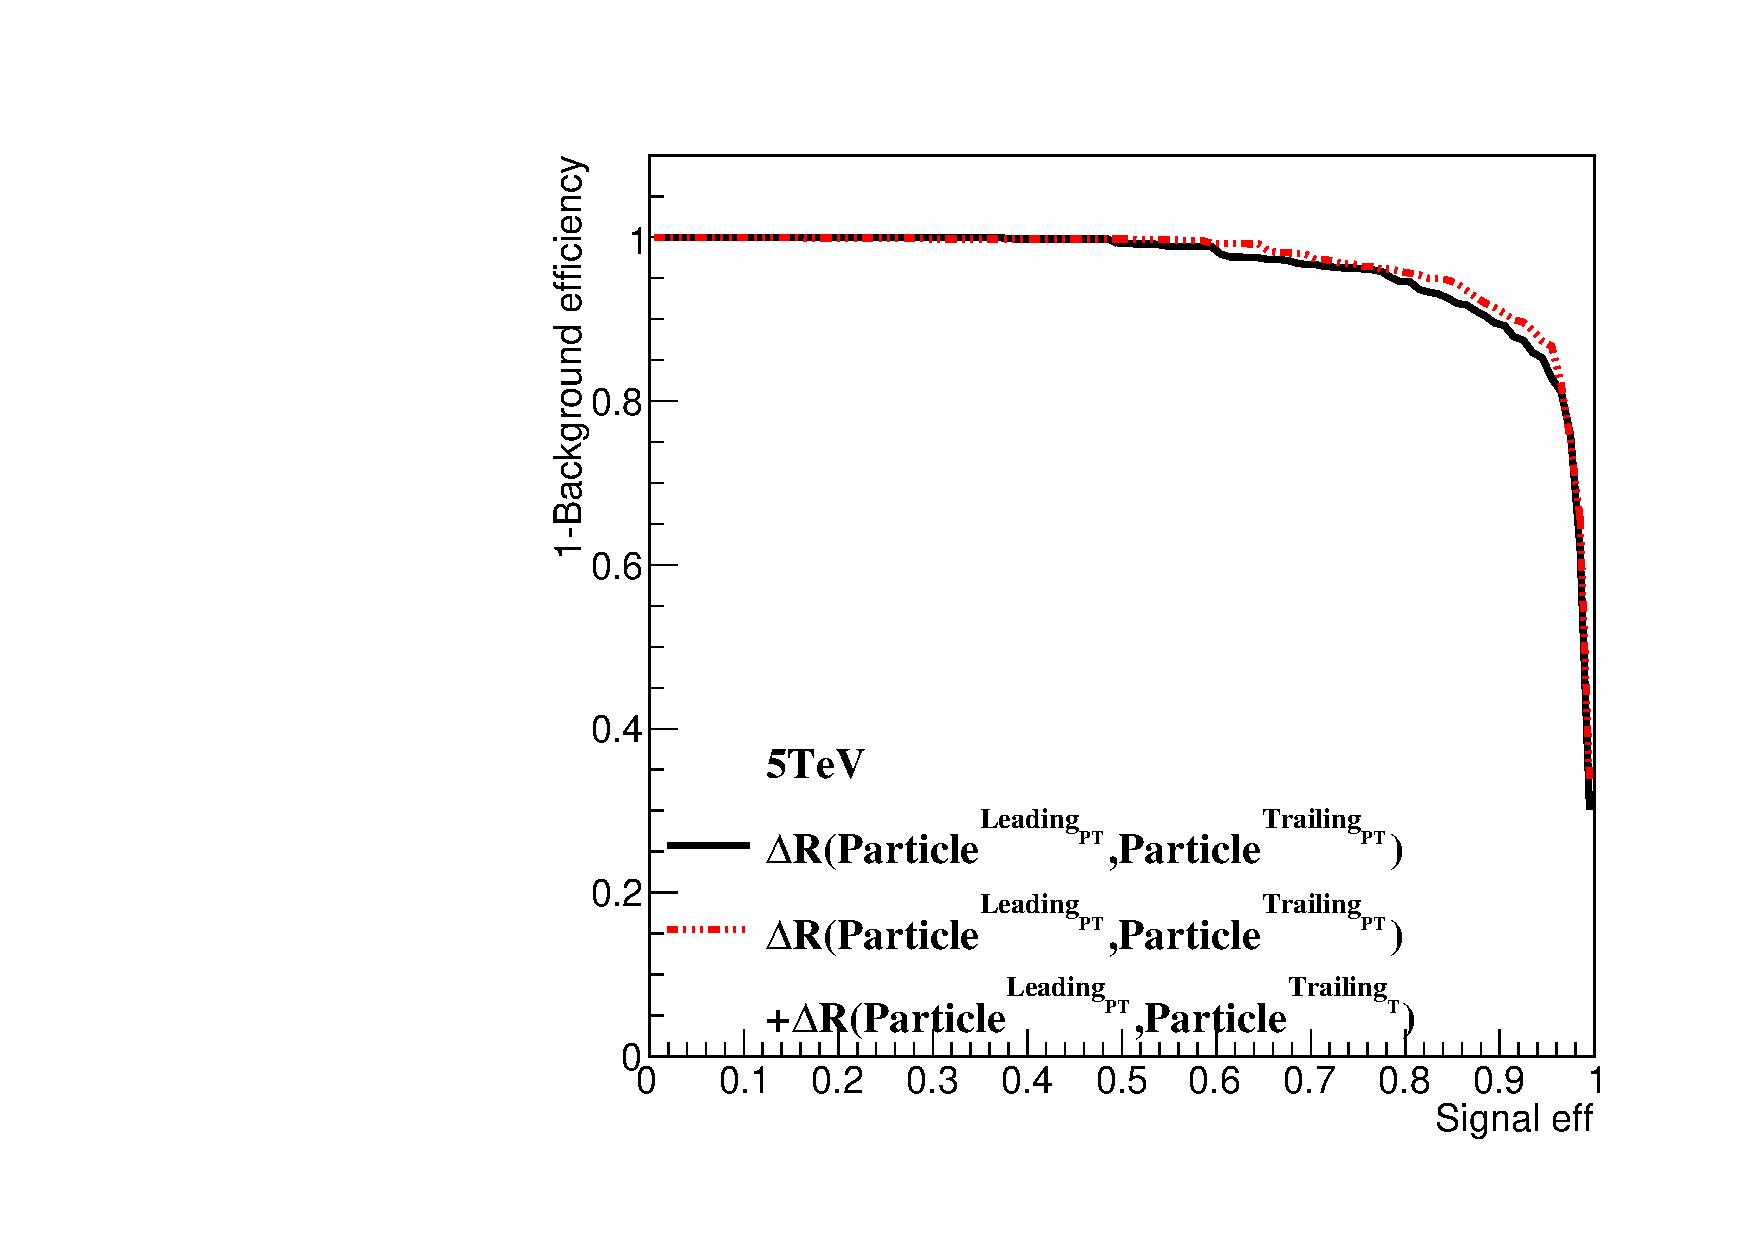
\includegraphics[width=0.4\textwidth]{/Users/ms08962476/Timing_paper/Pictures_used_for_FCC_and_jets/Truth_dR_BDT/BDT_plot_dR_dRplusID_5TeV_Truth.pdf}
   }
   \subfigure[10TeV] {
   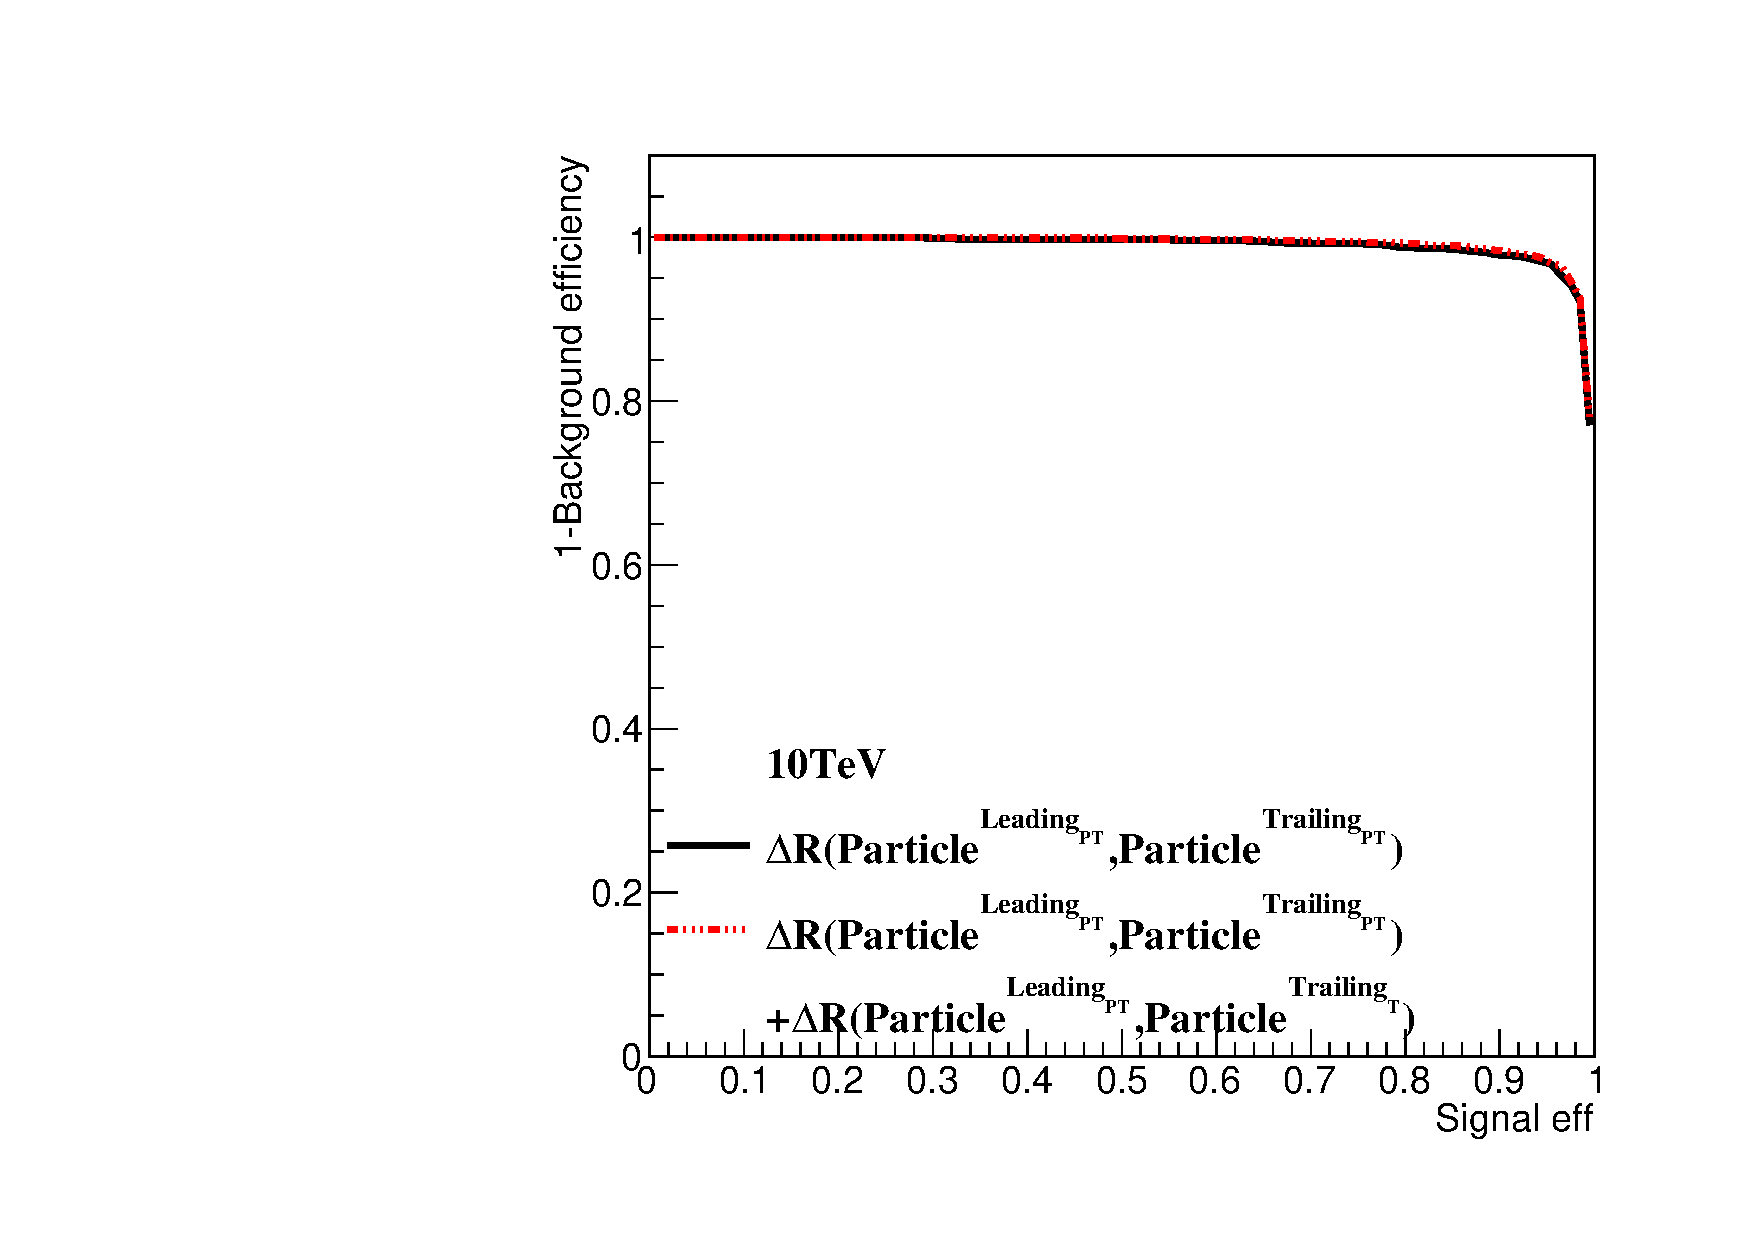
\includegraphics[width=0.4\textwidth]{/Users/ms08962476/Timing_paper/Pictures_used_for_FCC_and_jets/Truth_dR_BDT/BDT_plot_dR_dRplusID_10TeV_Truth.pdf}
   }
   \subfigure[20TeV] {
   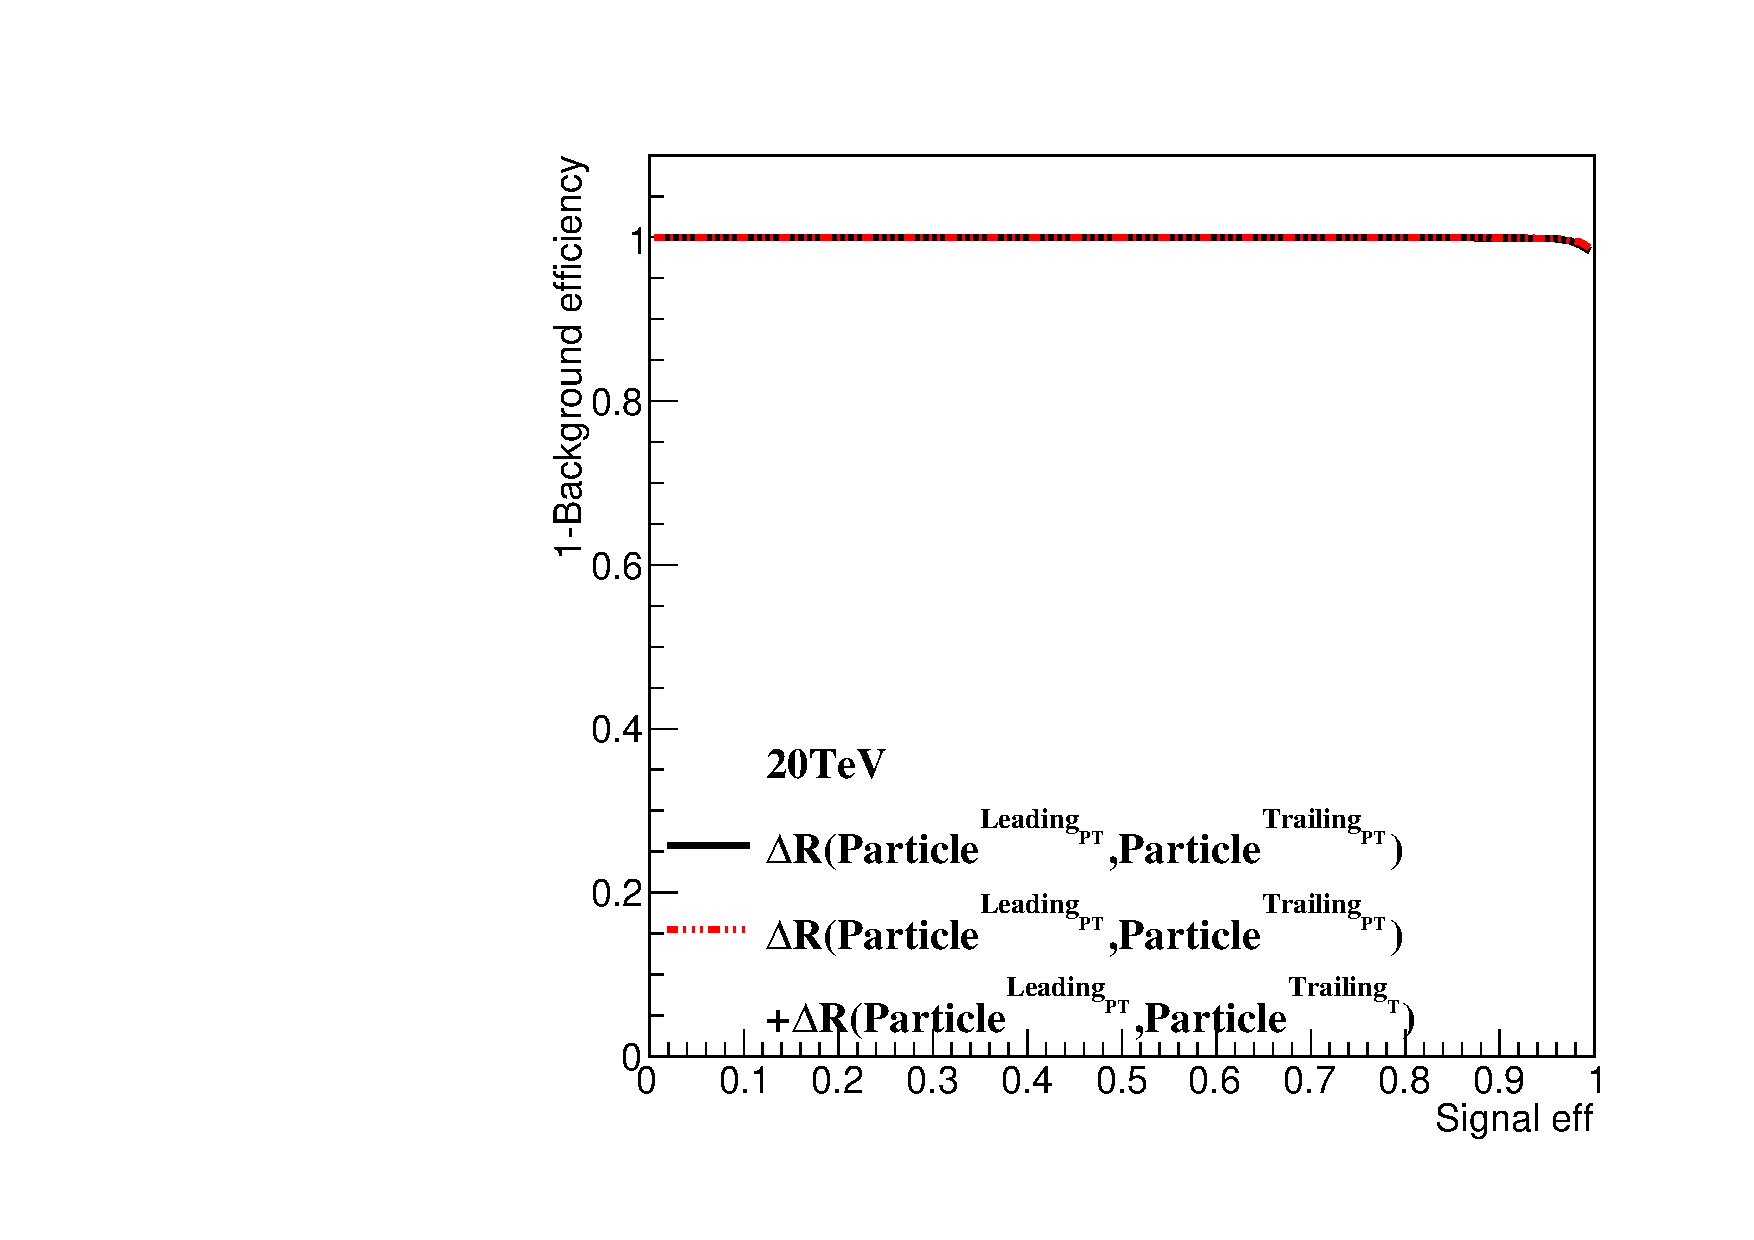
\includegraphics[width=0.4\textwidth]{/Users/ms08962476/Timing_paper/Pictures_used_for_FCC_and_jets/Truth_dR_BDT/BDT_plot_dR_dRplusID_20TeV_Truth.pdf}
   }
      \subfigure[40TeV] {
   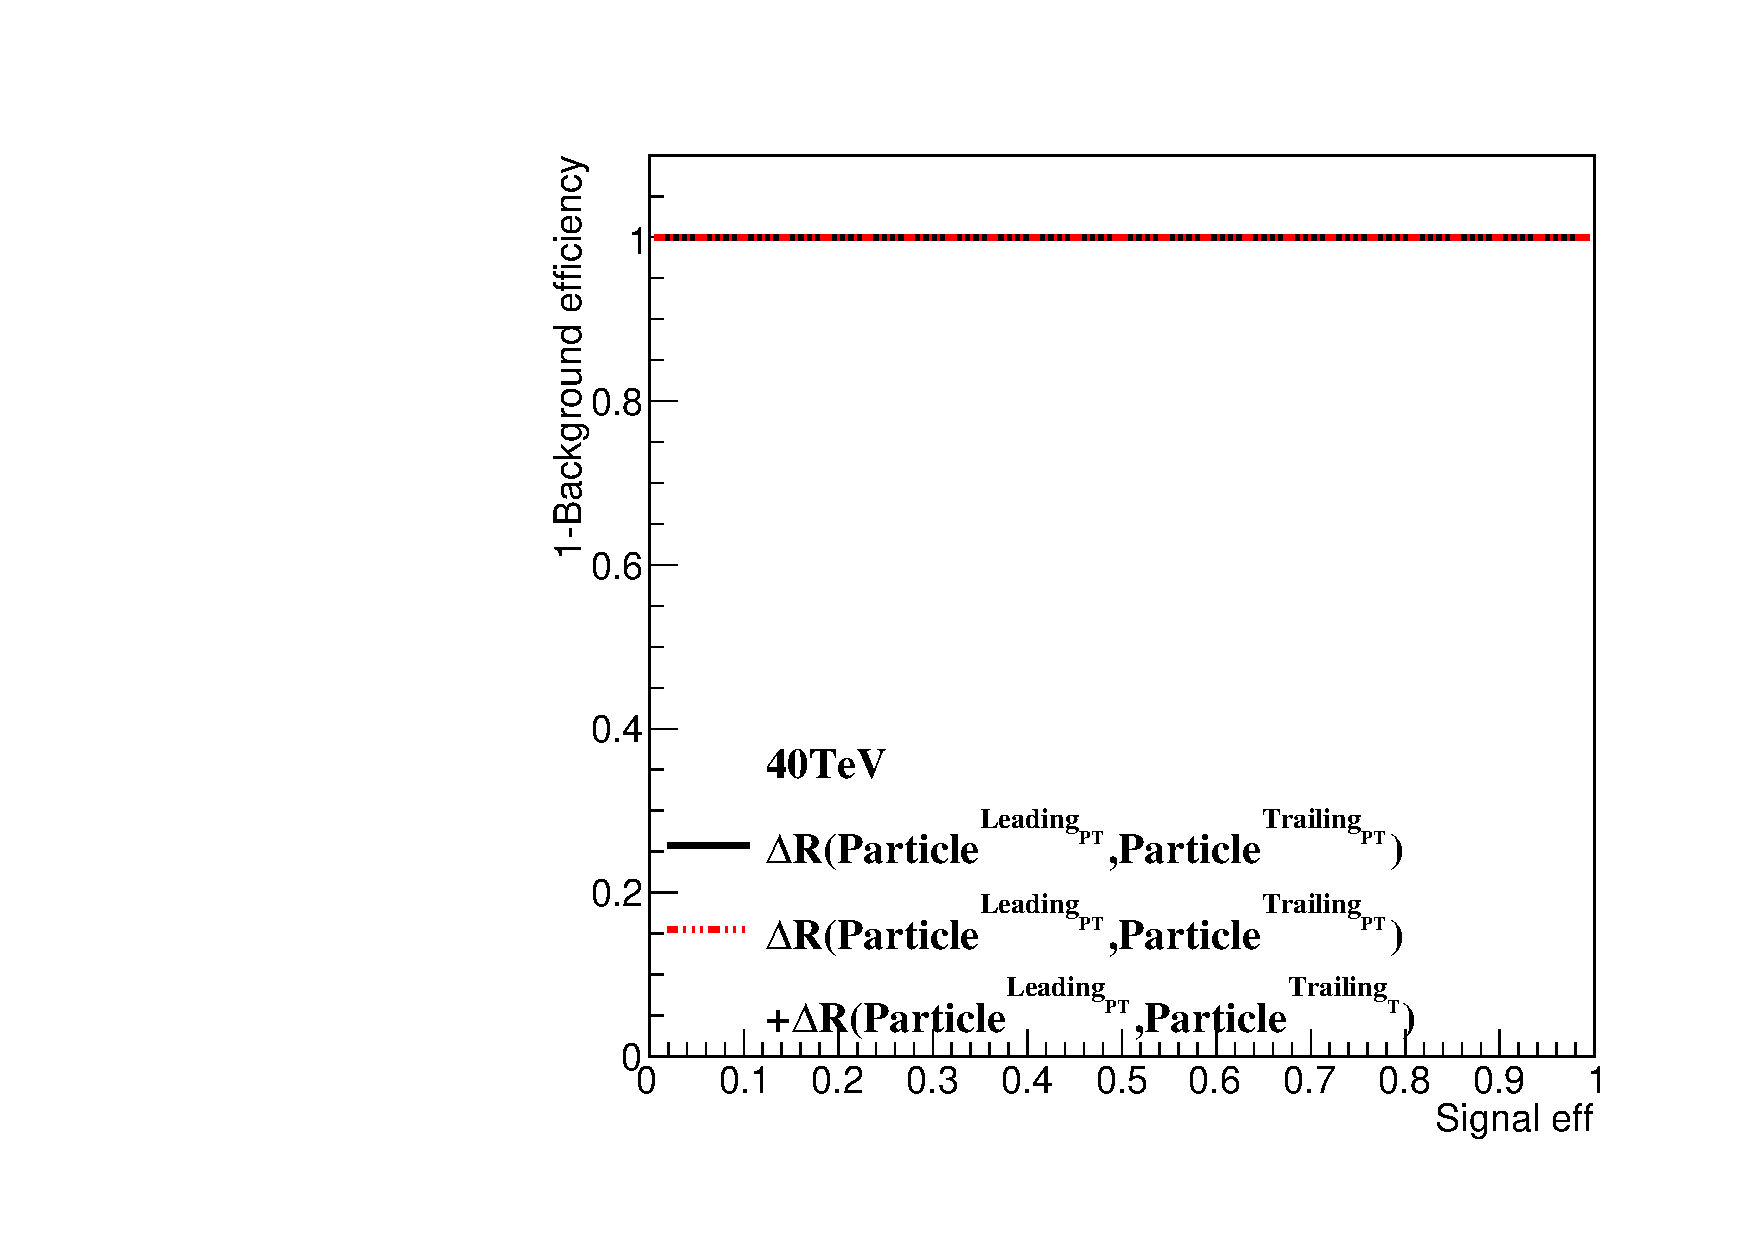
\includegraphics[width=0.4\textwidth]{/Users/ms08962476/Timing_paper/Pictures_used_for_FCC_and_jets/Truth_dR_BDT/BDT_plot_dR_dRplusID_40TeV_Truth.pdf}
   }
\end{center}
\caption{The comparison of the ROC curves obtained from two cases including five trailing-$P_{T}$ particles up to the fifth order alone(black) and the ones accompanied by five trailing-T particles up to the fifth order(red) with  the truth information of the different $M(Z')$ are shown here. The signal (background) process is $Z'\rightarrow WW$ ($Z' \rightarrow q\bar{q}$).\label{fig:Truth_dR_BDT}}
\end{figure}


For the distributions of Z'$\rightarrow$qq of both resonance masses, the mass-independent extensive shapes ranging from 0 to 0.2 can be easily recognized in all cases. Oppositely, the mass-dependent distributions of $\Delta R$ observed by the Z'$\rightarrow$WW can be acquainted conspicuously. The lower mass case of Z'$\rightarrow$WW at 5TeV shown in Fig \ref{fig:Truth_dR_Dis_5TeV_PT} and Fig.\ref{fig:Truth_dR_Dis_5TeV_T} shows the very different behavior compared with the ones acquired from 40TeV case, which is illustrated in Fig.\ref{fig:Truth_dR_Dis_40TeV_PT} and Fig \ref{fig:Truth_dR_Dis_40TeV_T} displaying the very narrow distributions centralizing near the 0. Those schemes can be used as a proof of $\Delta R$ is the great variable for distinguishing the different subjet cases by the large-separation appearance obtained from the higher mass case. \\

After performing the separation power of $\Delta R$ with the histograms qualitatively, the quantitive way with the module of the Boosted Decision Tree(BDT) will be utilized as investigating the power of the discrimination for all four resonance masses. In the Fig.\ref{fig:Truth_dR_BDT}, the BDT method is applied to make out the efficiency of separating the two processes with the input variables of those trailing particles up to the fifth order defined by T and PT for all cases. The statement which can be addressed from the plots is that the separation power of the $\Delta R$ with trailing-$P_{T}$ is as perfect as trailing-T, originating from the lines overlap together in the figure. In this case, the variable of $\Delta R$ is worthy for us to keep exploring on to see whether the cases are similar as the ones done with the reco-level data.\\

%With regard to taking advantage of the timing ideally, the other one is to take it as the tool of identifying the particles. The plots of Fig\ref{} and Fig\ref{} show the distribution of the particle ID with respect to the trailing-$P_{T}$ and trailing-T cases, the another function found favorable is that the protons can be tagged more within the cases of the Trailing-T. For the purpose of quantifying them, we manage 


\subsection{The Reco-level cases}
Over the specific studies for the $\Delta R$ with the truth-level information in the former section, the capability of the $\Delta R$ with the timing is aware of as a a great variable as $P_{T}$ into investigating the different number of the subjets within a large radius jet. Followed up by that, the essential step of verifying on the efficiency of the variable applied in the real case is to prepare the reco-level data, which serves as the situations operating in the future, to corroborate the advanced of the timing employed into handling the issue.\\ 

The distributions of the $\Delta R$, which are revealed from Fig.\ref{fig:Reco_dR_Dis_5TeV_PT} to Fig.\ref{fig:Reco_dR_Dis_40TeV_T} for 5TeV and 40TeV cases as the ones used in the truth-level studies, show that the distributions of Z'$\rightarrow$WW and Z'$\rightarrow$qq can't be well-separated by both trailing cases sharply at the higher C.M. point, and that is caused by the non-smearing detector resulting in the possible outcome of the $\Delta R$ can only be the value of any two-cells angle of ECAL but not the authentic truth particles . Surprisingly, the timing in this case can give us a little bit improvement upon the $P_{T}$ cases with the proof of the BDT plots in Fig.\ref{fig:Reco_dR_BDT} summarizing the efficiency of those variables. Much improvement with the timing can be observed at the higher C.M. point.\\

\begin{figure}
\begin{center}
   \subfigure[The first trailing-PT] {
   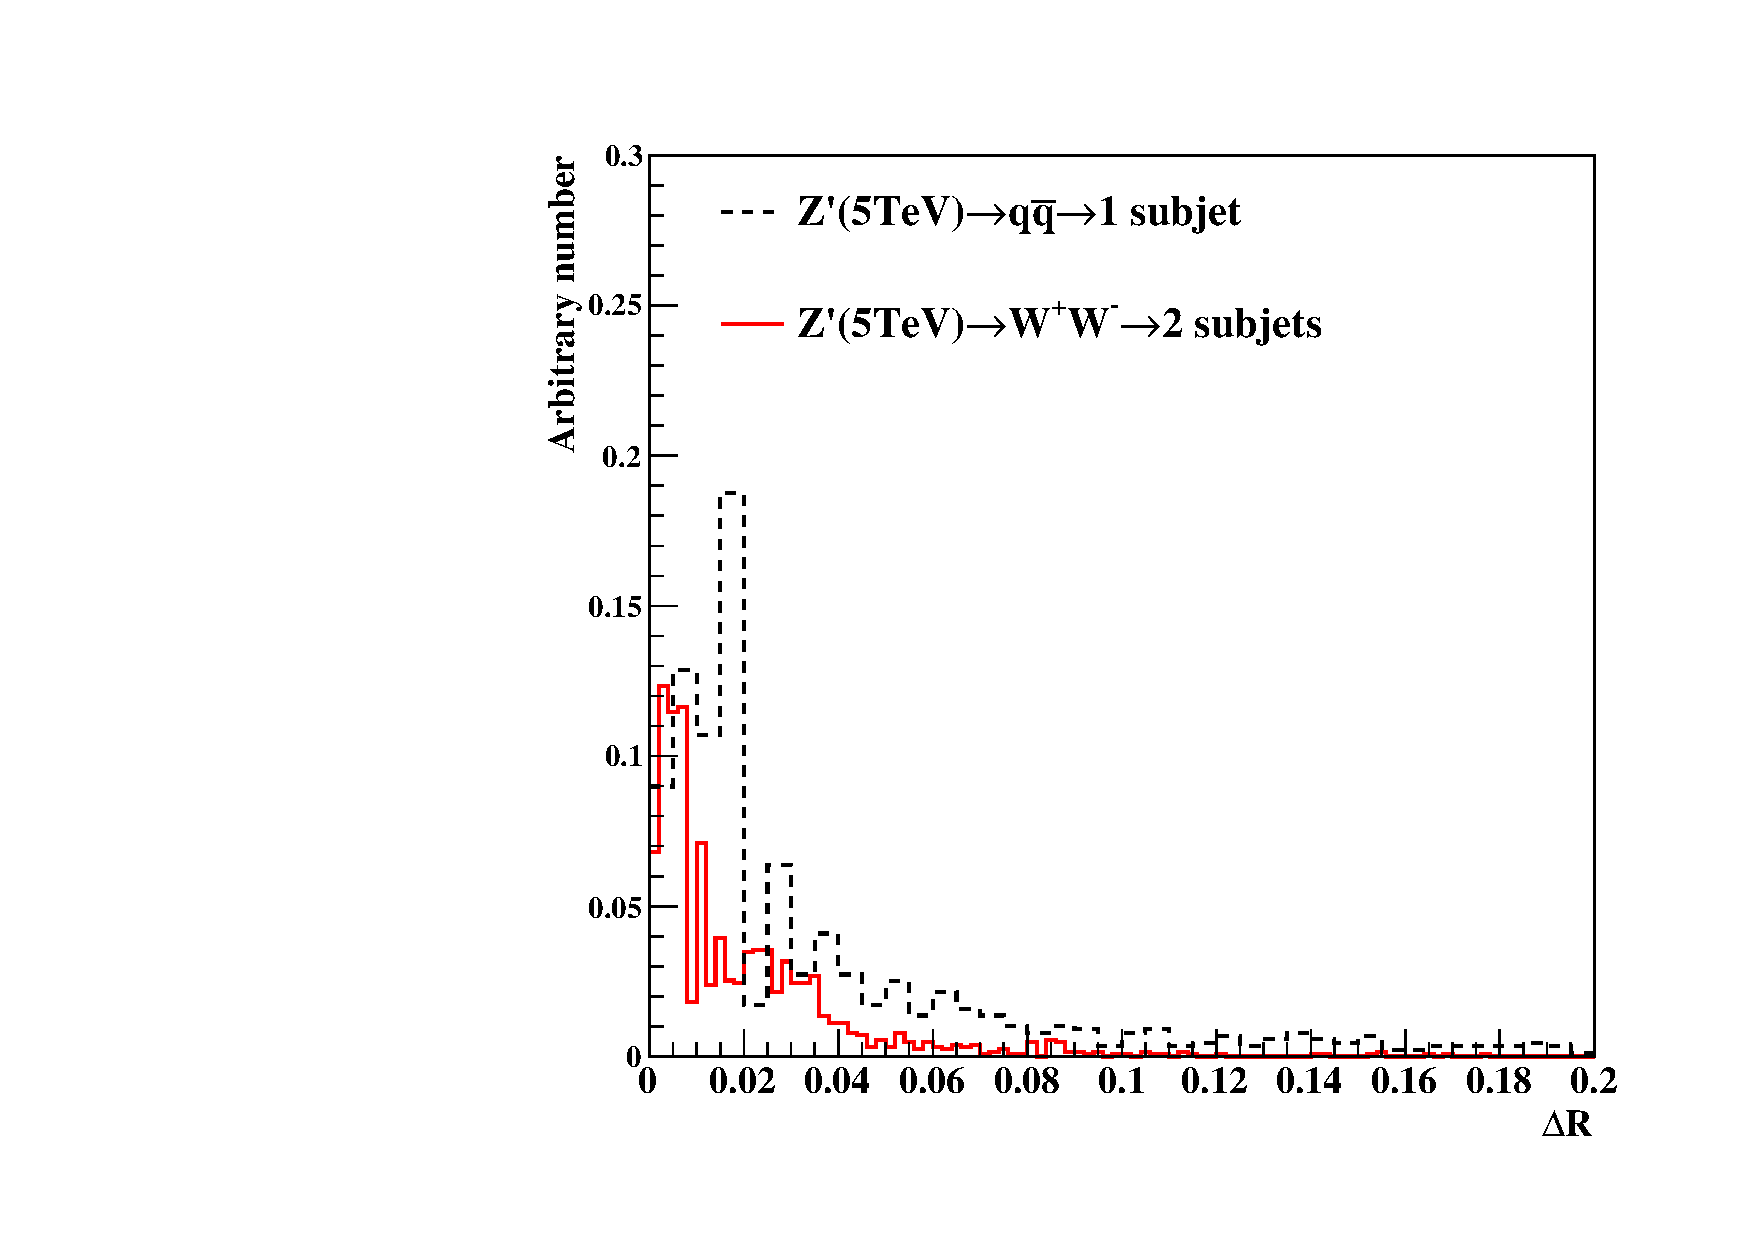
\includegraphics[width=0.3\textwidth]{/Users/ms08962476/Timing_paper/Pictures_used_for_FCC_and_jets/Reco_dR_Dis_ECAL/5TeV_Reco/dR_PT_0_5TeV_Reco.pdf}
   }
   \subfigure[The second trailing-T] {
   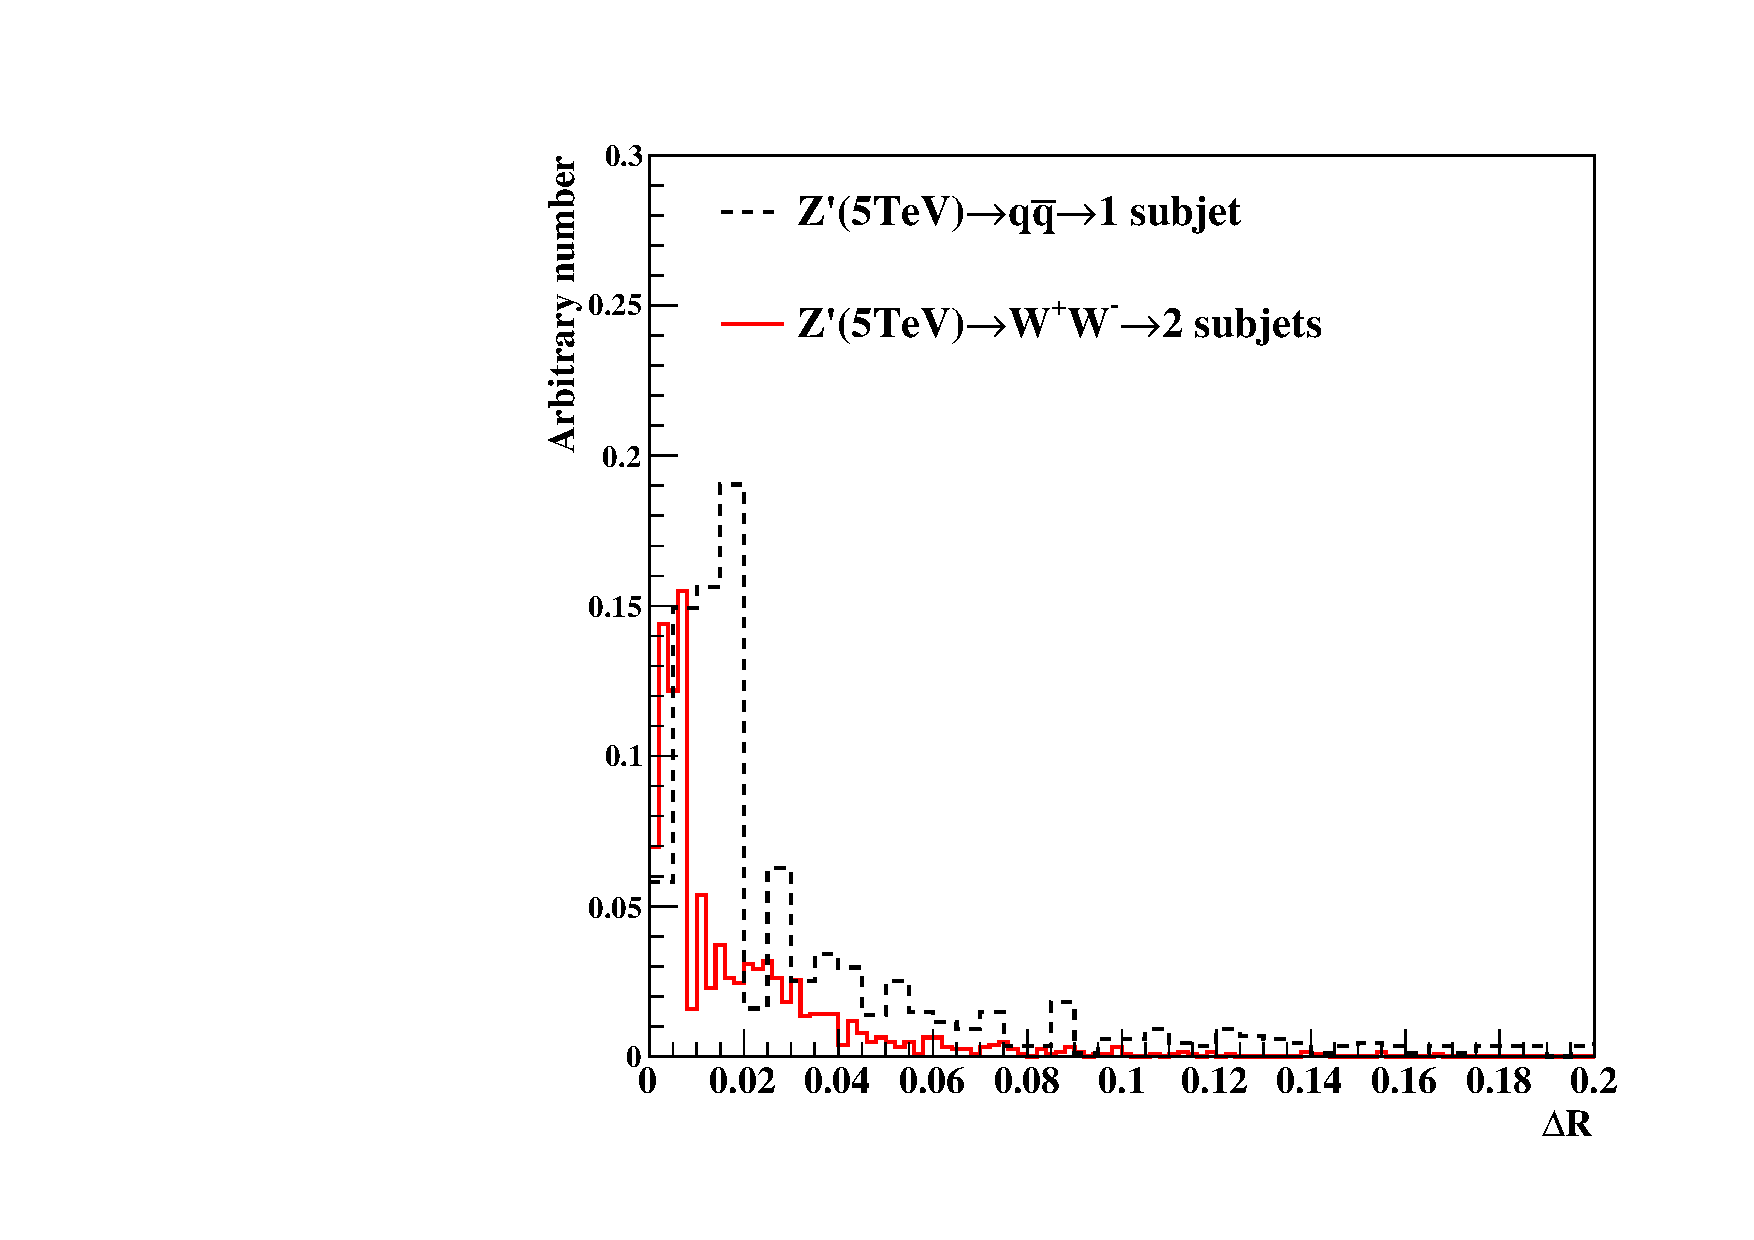
\includegraphics[width=0.3\textwidth]{/Users/ms08962476/Timing_paper/Pictures_used_for_FCC_and_jets/Reco_dR_Dis_ECAL/5TeV_Reco/dR_PT_1_5TeV_Reco.pdf}
   }
   \subfigure[The third trailing-T] {
   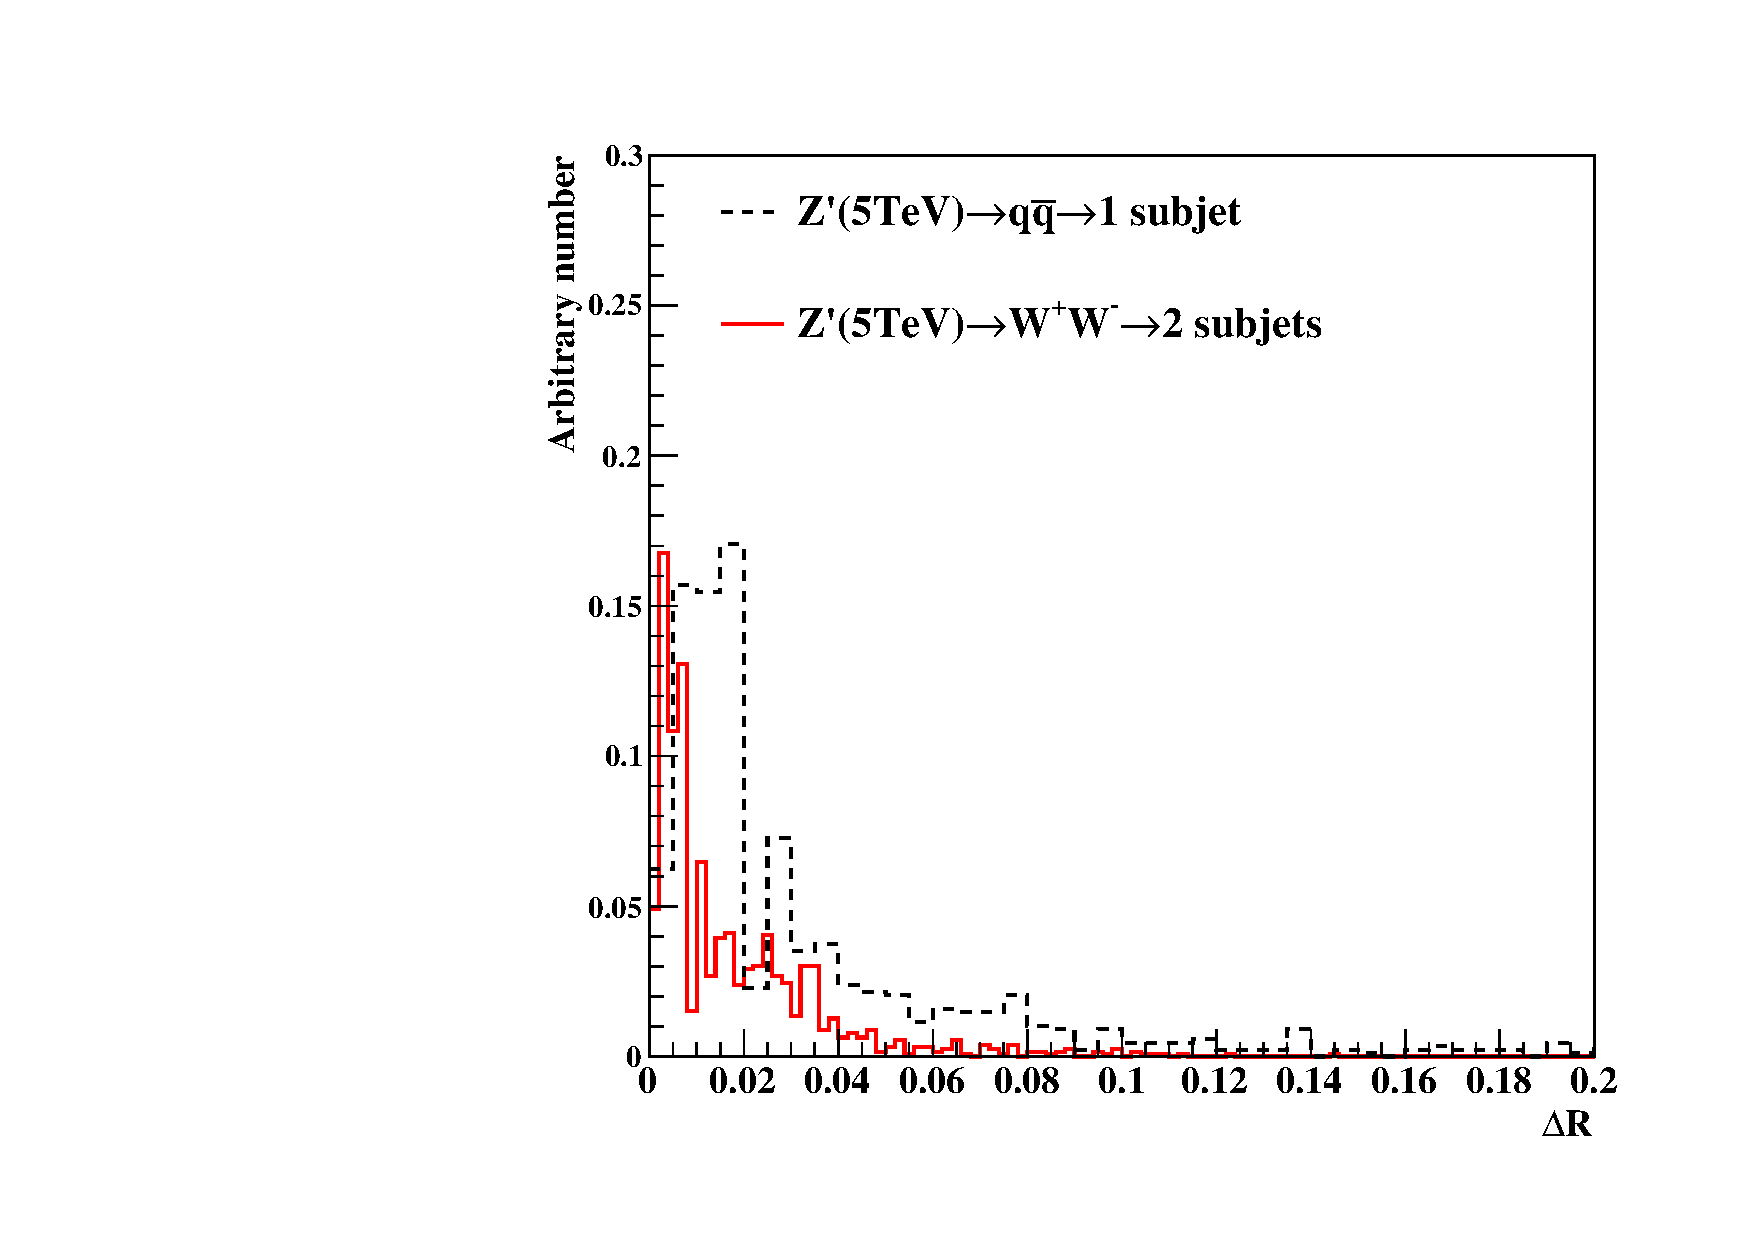
\includegraphics[width=0.3\textwidth]{/Users/ms08962476/Timing_paper/Pictures_used_for_FCC_and_jets/Reco_dR_Dis_ECAL/5TeV_Reco/dR_PT_2_5TeV_Reco.pdf}
   }
      \subfigure[The fourth trailing-T] {
   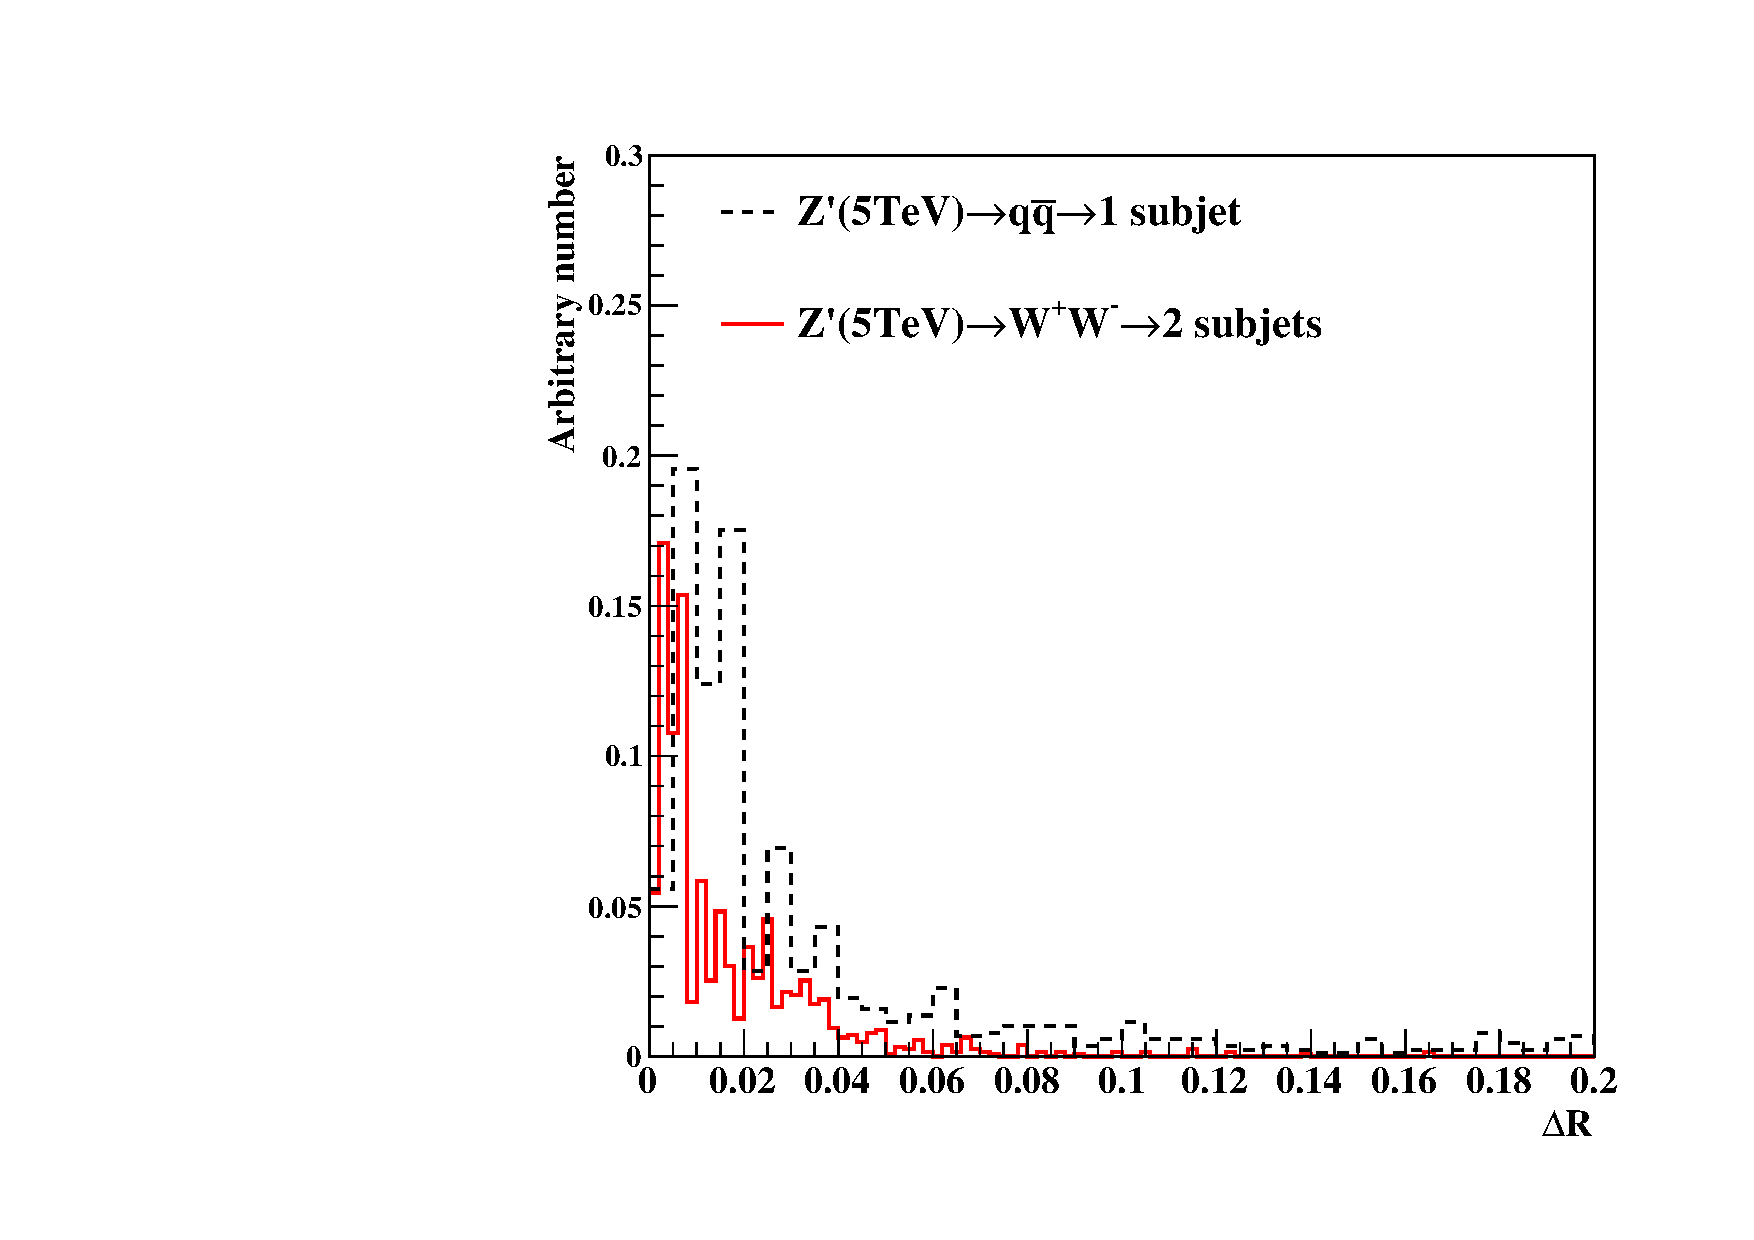
\includegraphics[width=0.3\textwidth]{/Users/ms08962476/Timing_paper/Pictures_used_for_FCC_and_jets/Reco_dR_Dis_ECAL/5TeV_Reco/dR_PT_3_5TeV_Reco.pdf}
   }
   \subfigure[The fifth trailing-T] {
   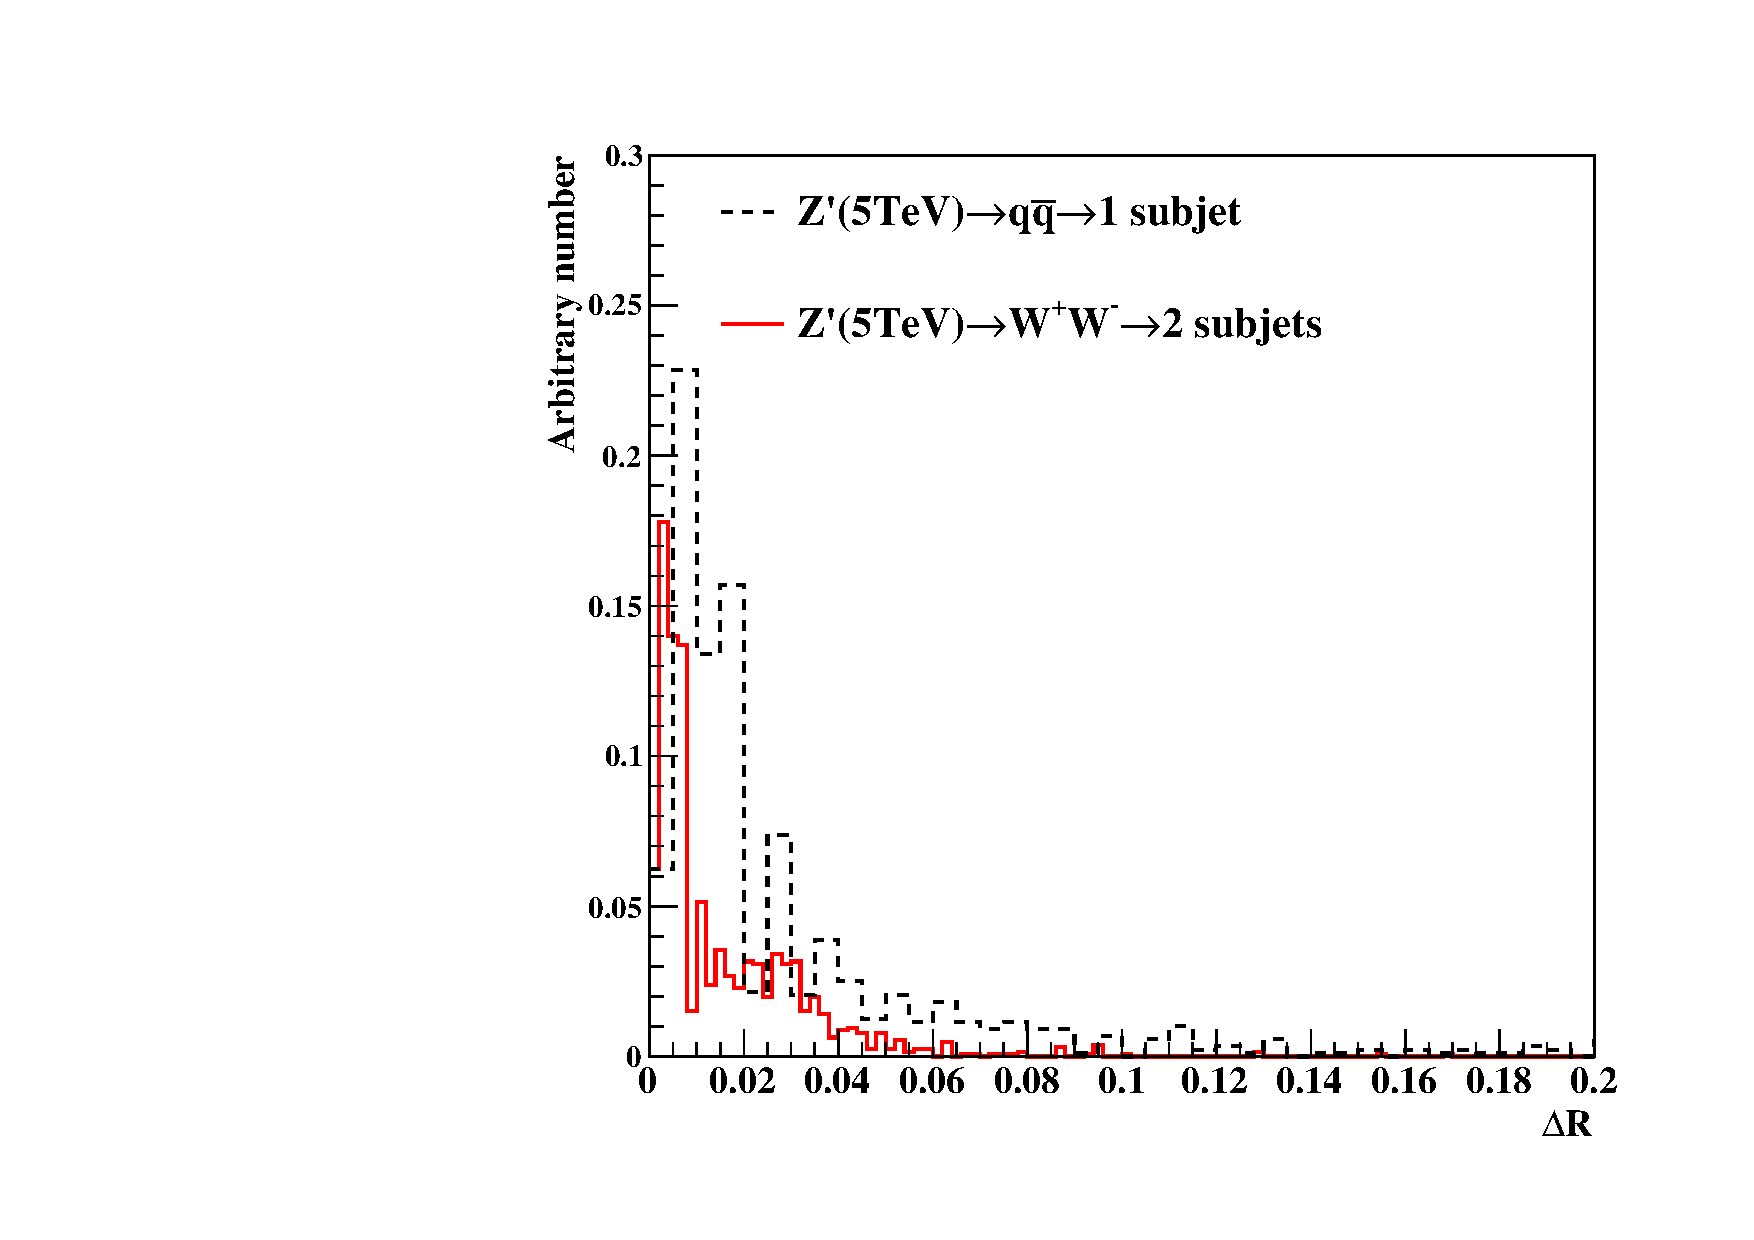
\includegraphics[width=0.3\textwidth]{/Users/ms08962476/Timing_paper/Pictures_used_for_FCC_and_jets/Reco_dR_Dis_ECAL/5TeV_Reco/dR_PT_4_5TeV_Reco.pdf}
   }
\end{center}
\caption{Distributions of $\Delta R$ for $M(Z') = 5$~TeV for five kinds of trailing-$P_{T}$ particles with the reco-level information of ECAL
are shown here. \label{fig:Reco_dR_Dis_5TeV_PT}}
\end{figure}

\begin{figure}
\begin{center}
   \subfigure[The first trailing-T] {
   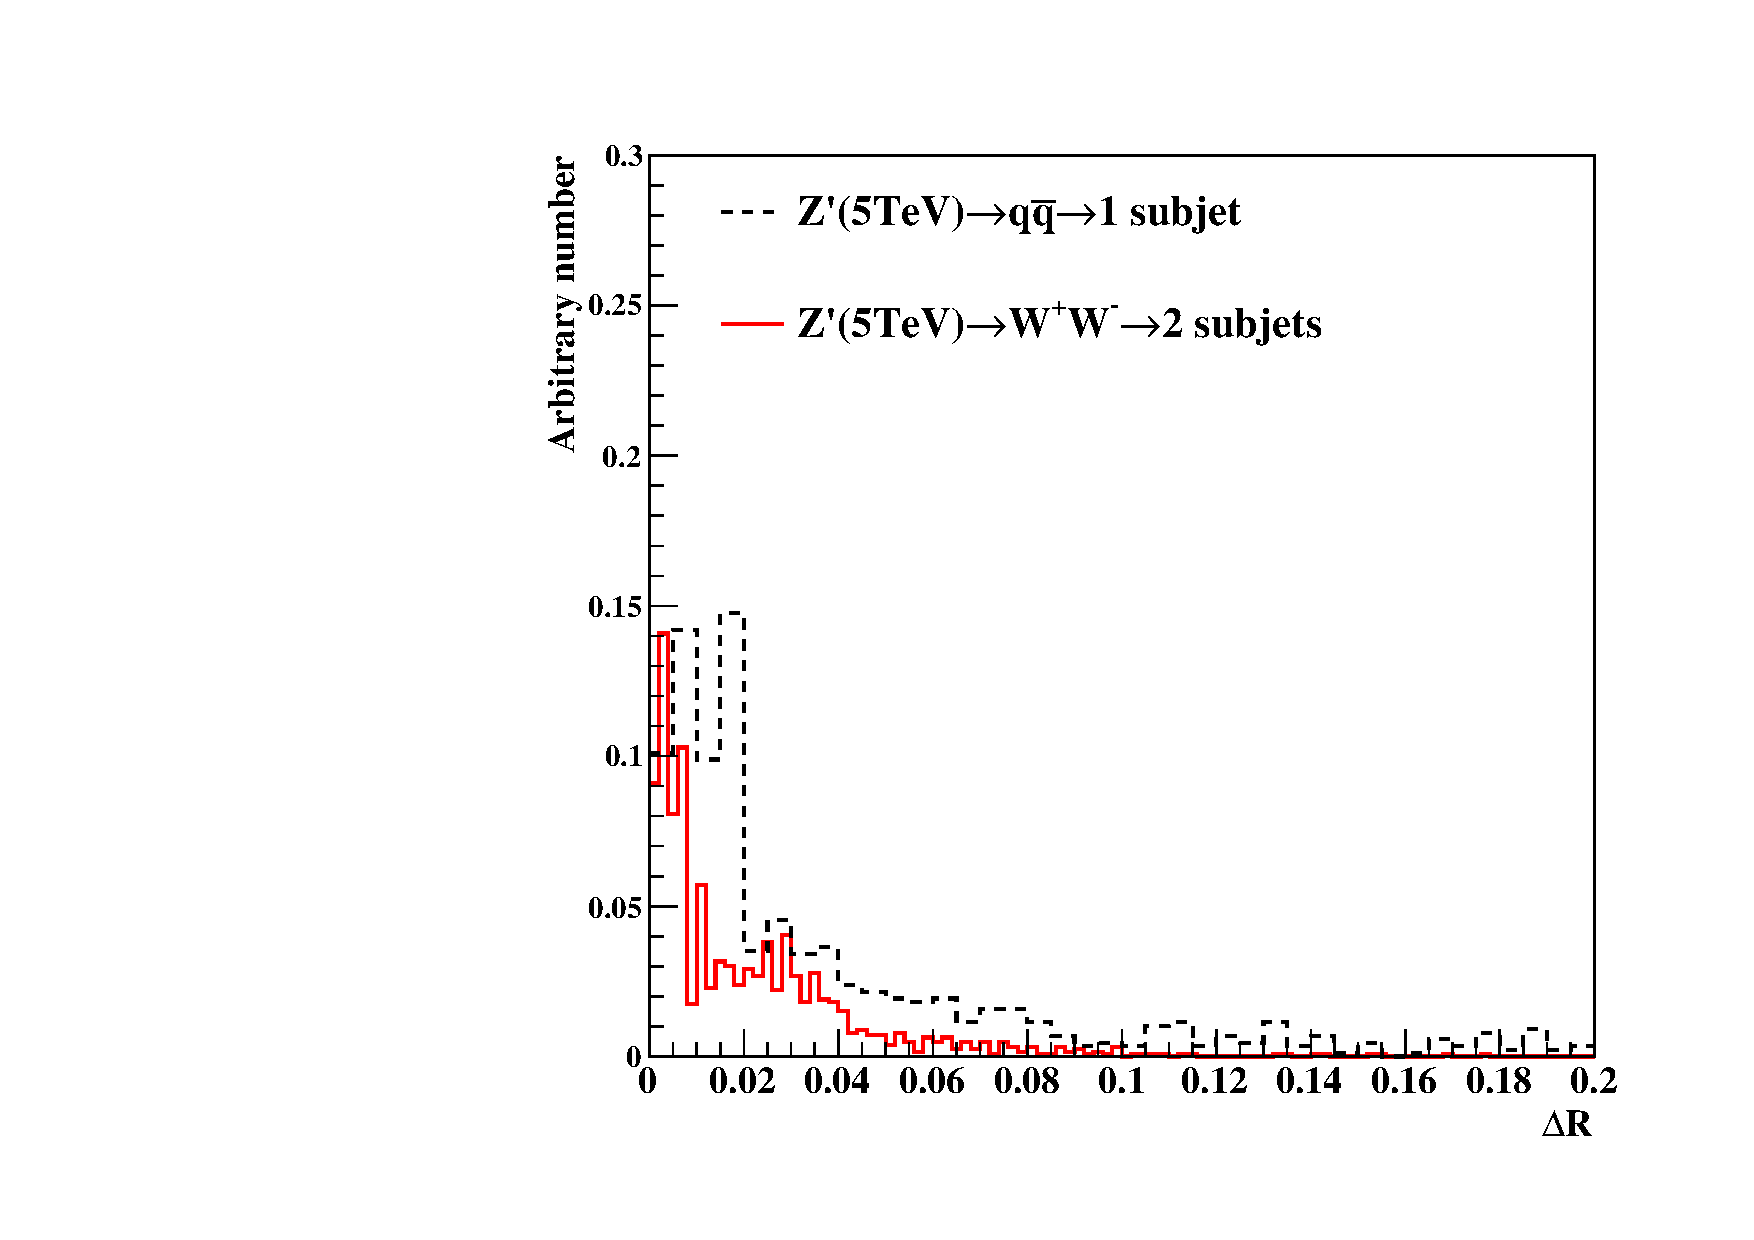
\includegraphics[width=0.3\textwidth]{/Users/ms08962476/Timing_paper/Pictures_used_for_FCC_and_jets/Reco_dR_Dis_ECAL/5TeV_Reco/dR_T_0_5TeV_Reco.pdf}
   }
   \subfigure[The second trailing-T] {
   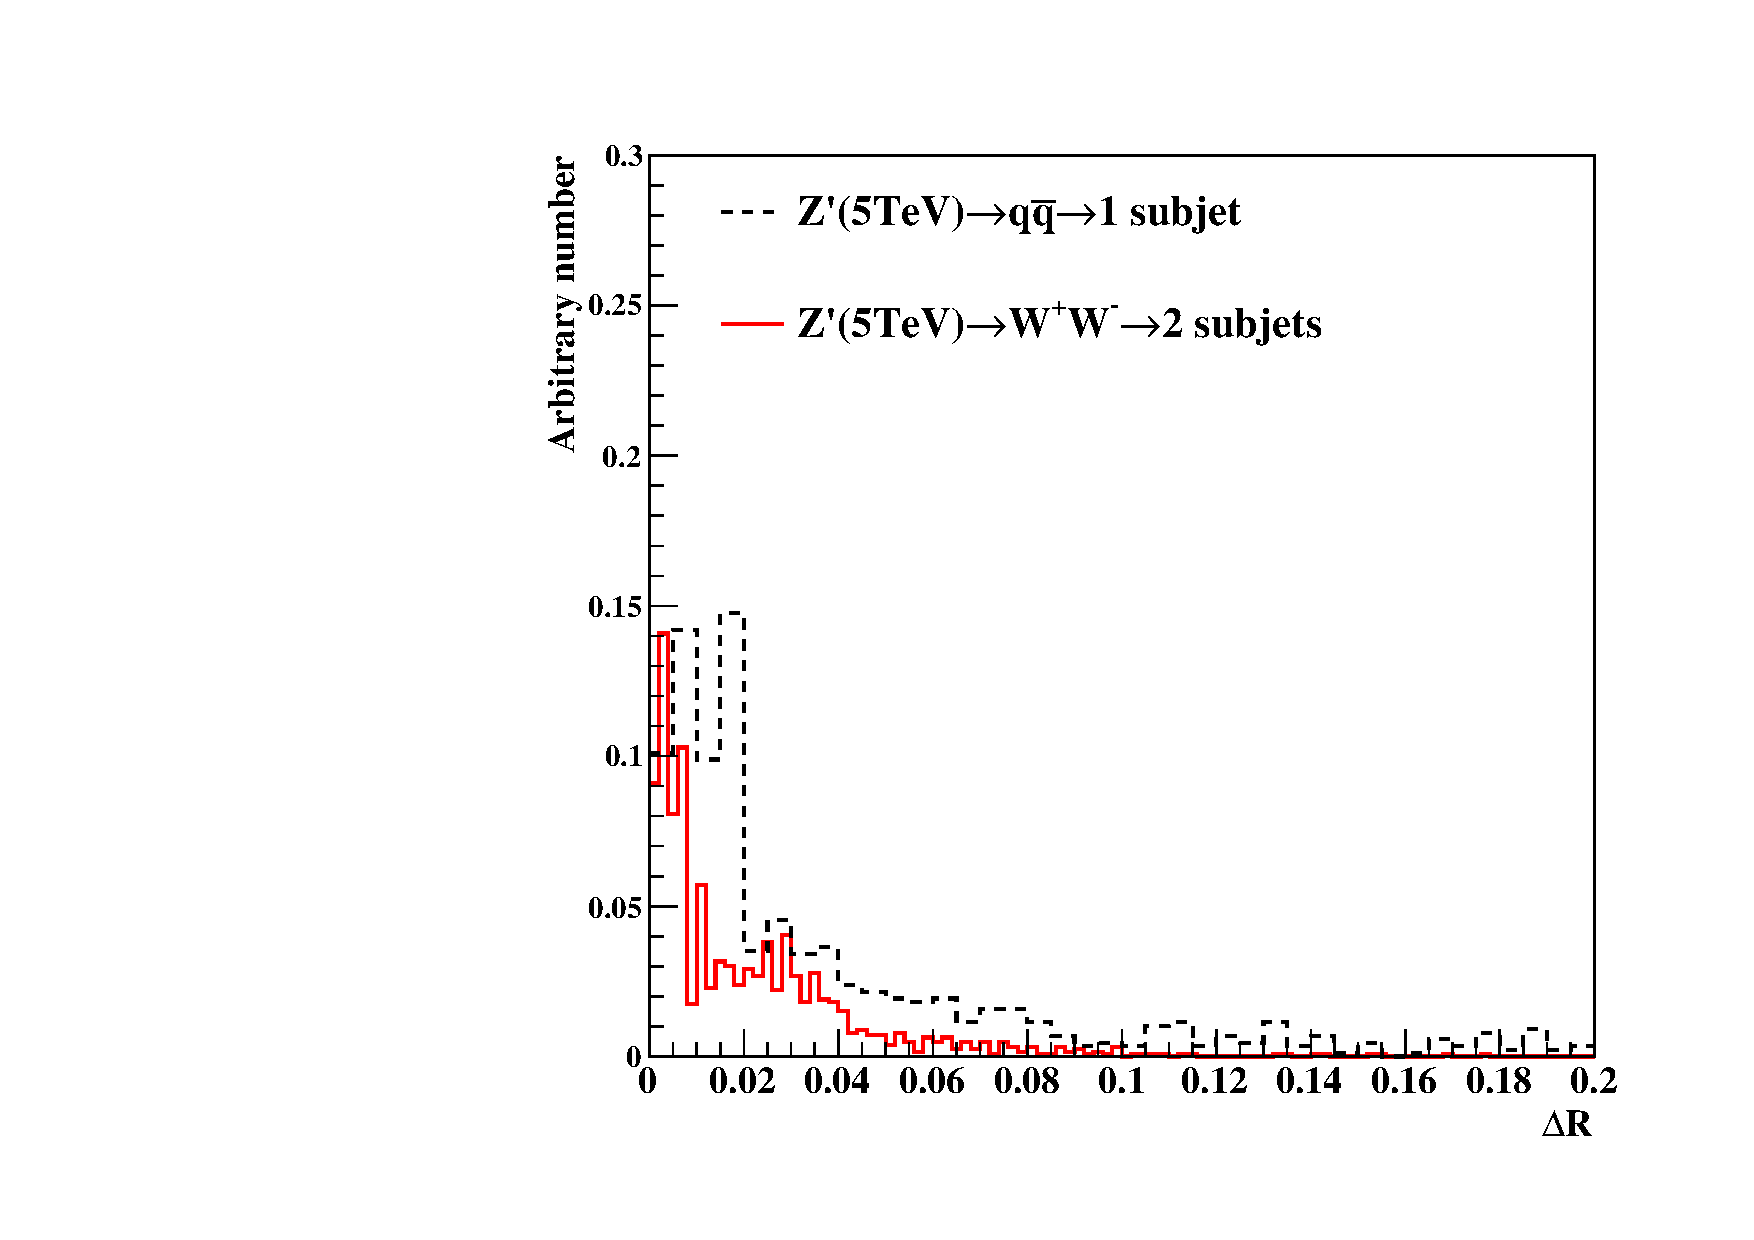
\includegraphics[width=0.3\textwidth]{/Users/ms08962476/Timing_paper/Pictures_used_for_FCC_and_jets/Reco_dR_Dis_ECAL/5TeV_Reco/dR_T_1_5TeV_Reco.pdf}
   }
   \subfigure[The third trailing-T] {
   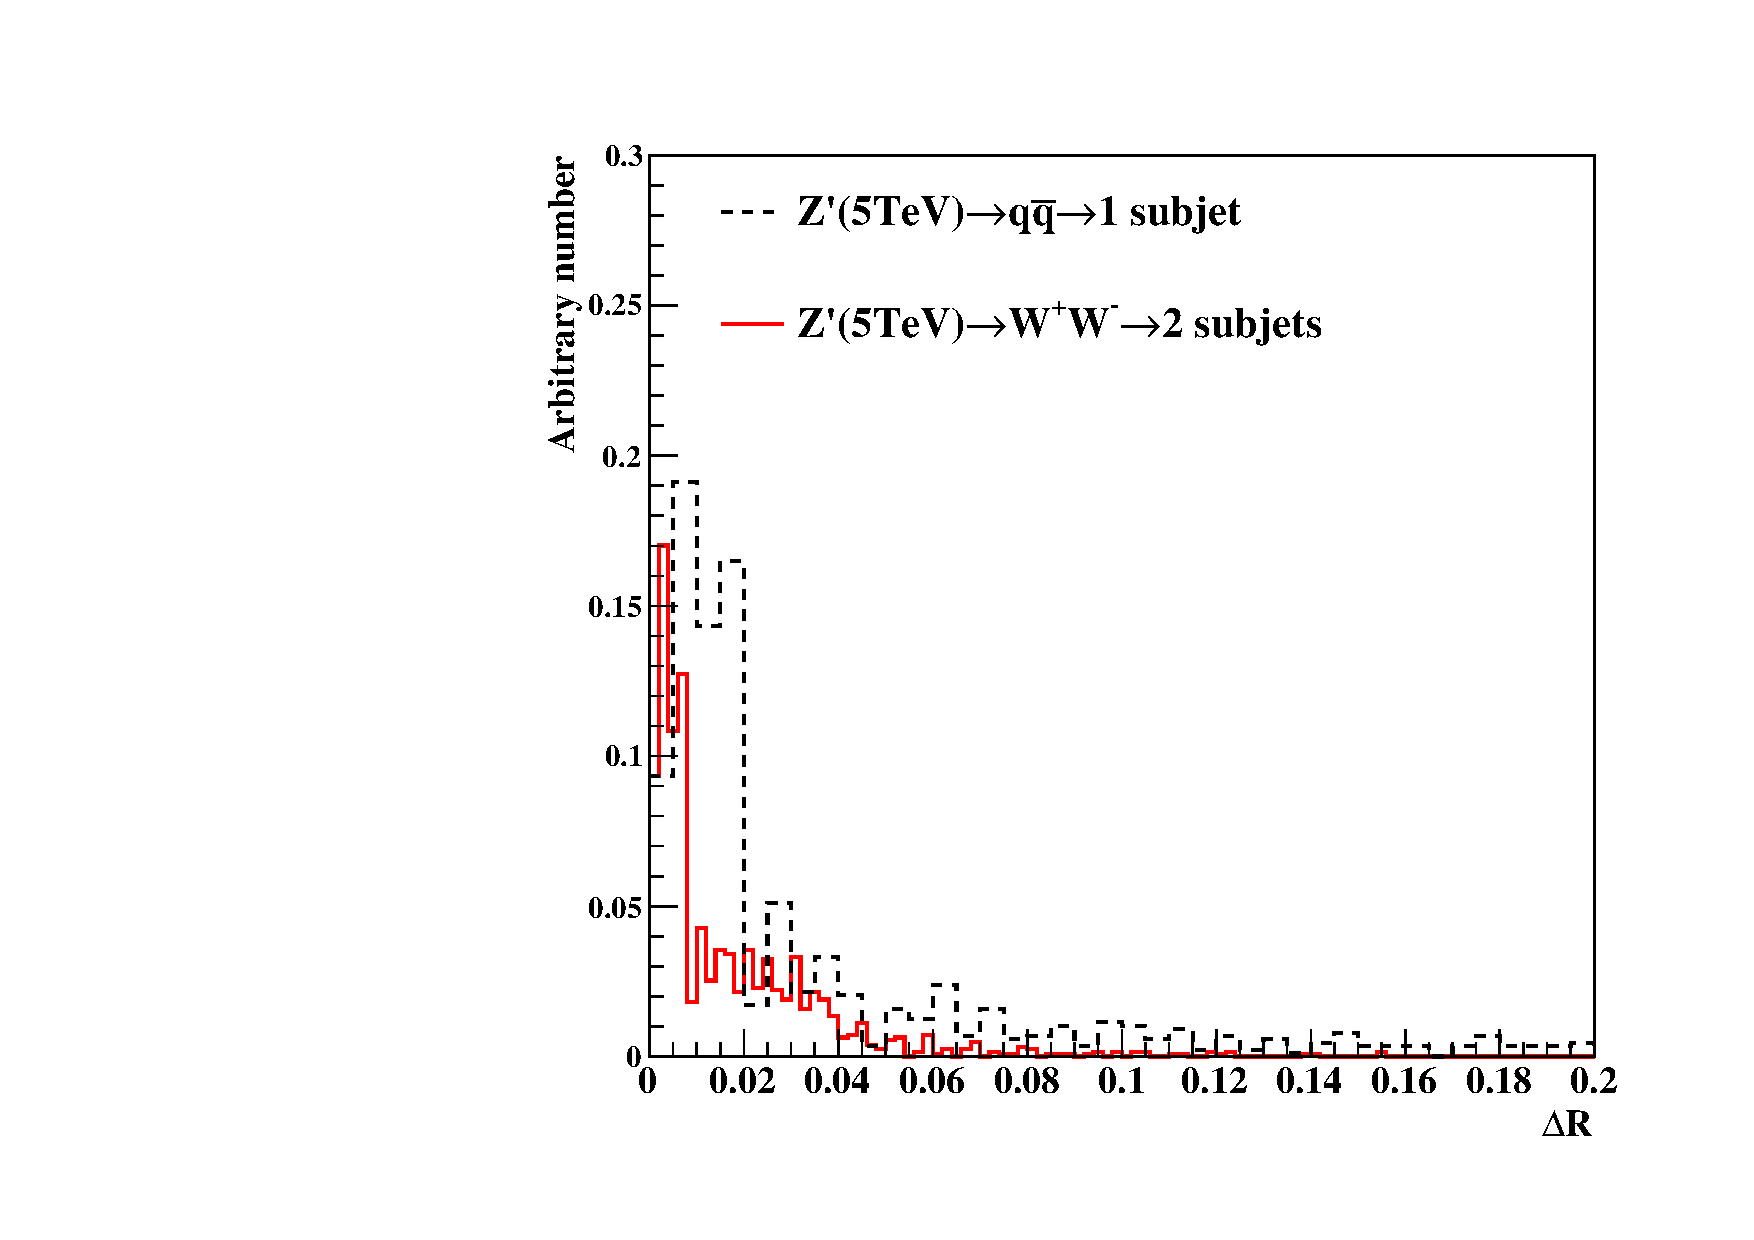
\includegraphics[width=0.3\textwidth]{/Users/ms08962476/Timing_paper/Pictures_used_for_FCC_and_jets/Reco_dR_Dis_ECAL/5TeV_Reco/dR_T_2_5TeV_Reco.pdf}
   }
      \subfigure[The fourth trailing-T] {
   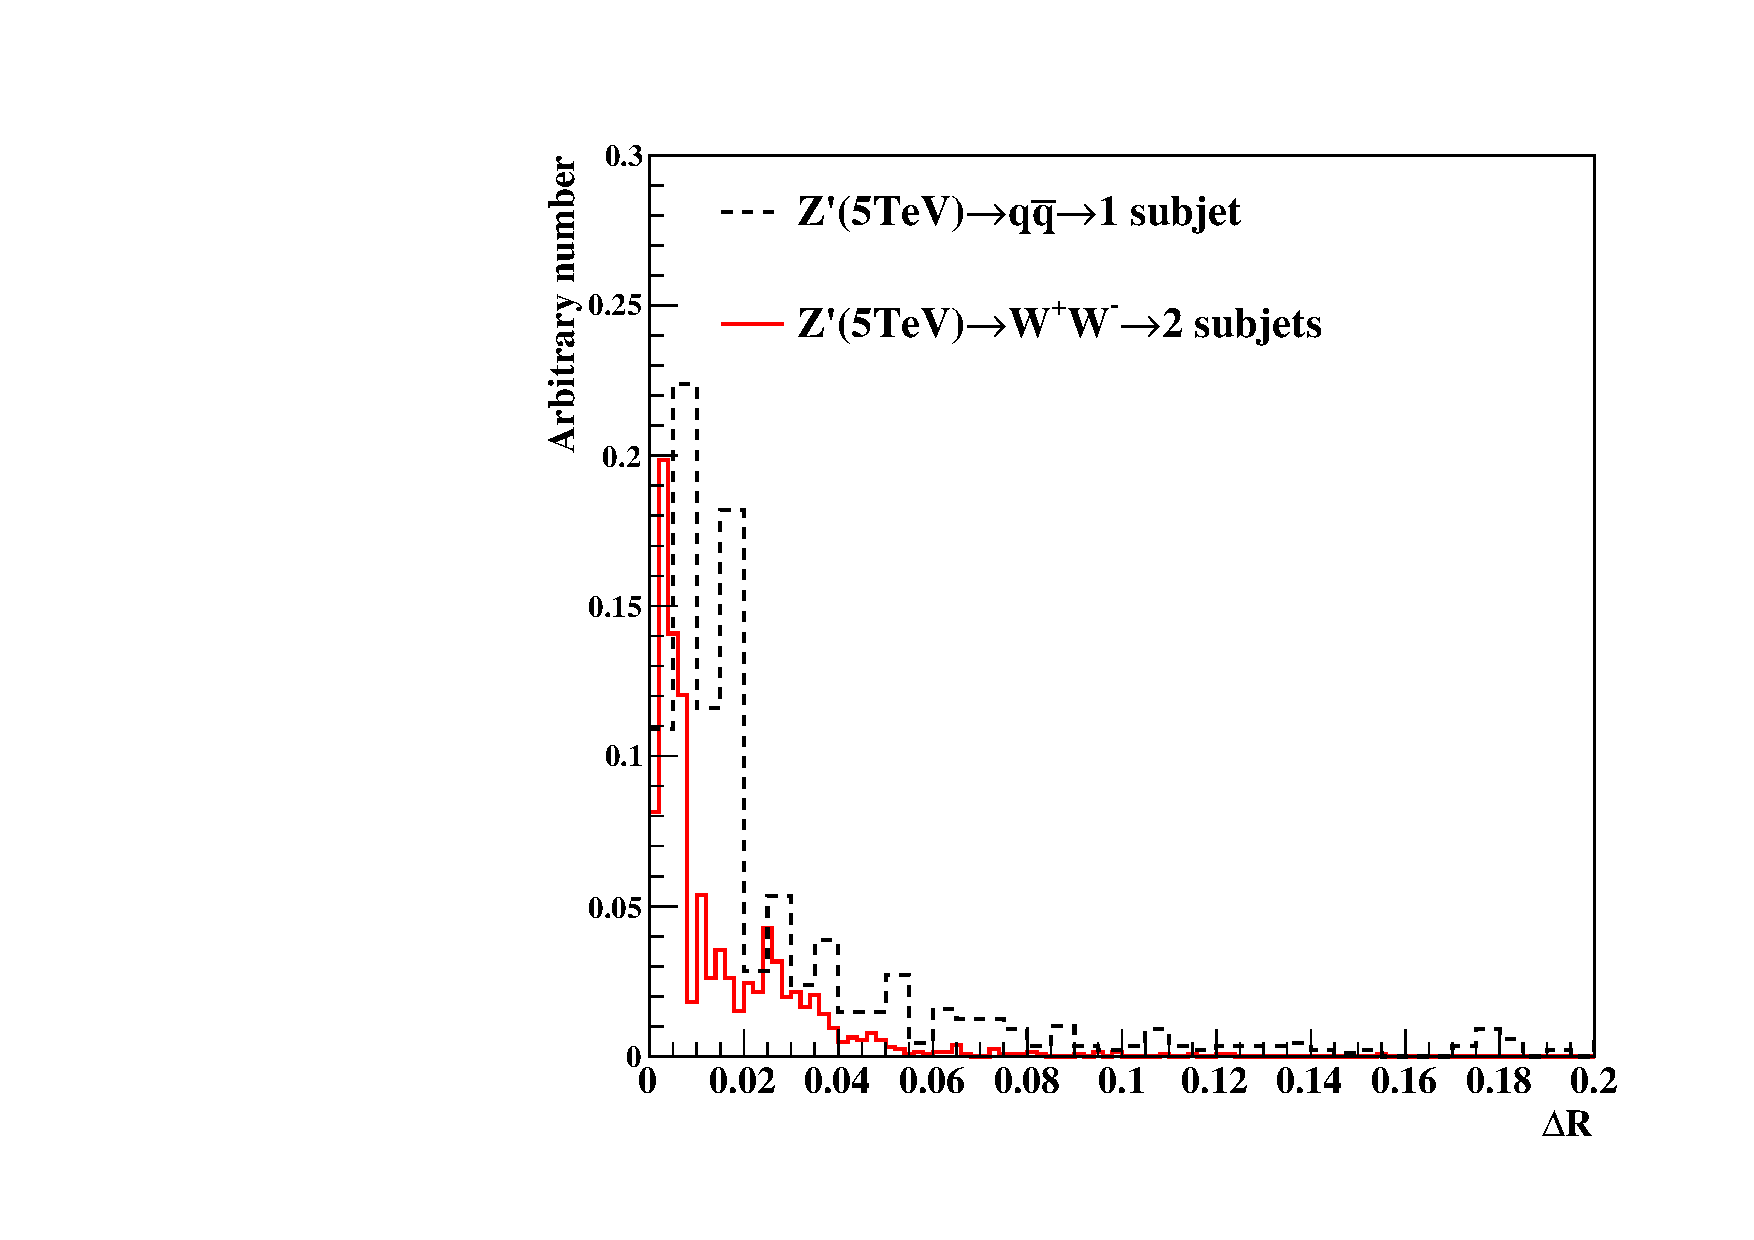
\includegraphics[width=0.3\textwidth]{/Users/ms08962476/Timing_paper/Pictures_used_for_FCC_and_jets/Reco_dR_Dis_ECAL/5TeV_Reco/dR_T_3_5TeV_Reco.pdf}
   }
   \subfigure[The fifth trailing-T] {
   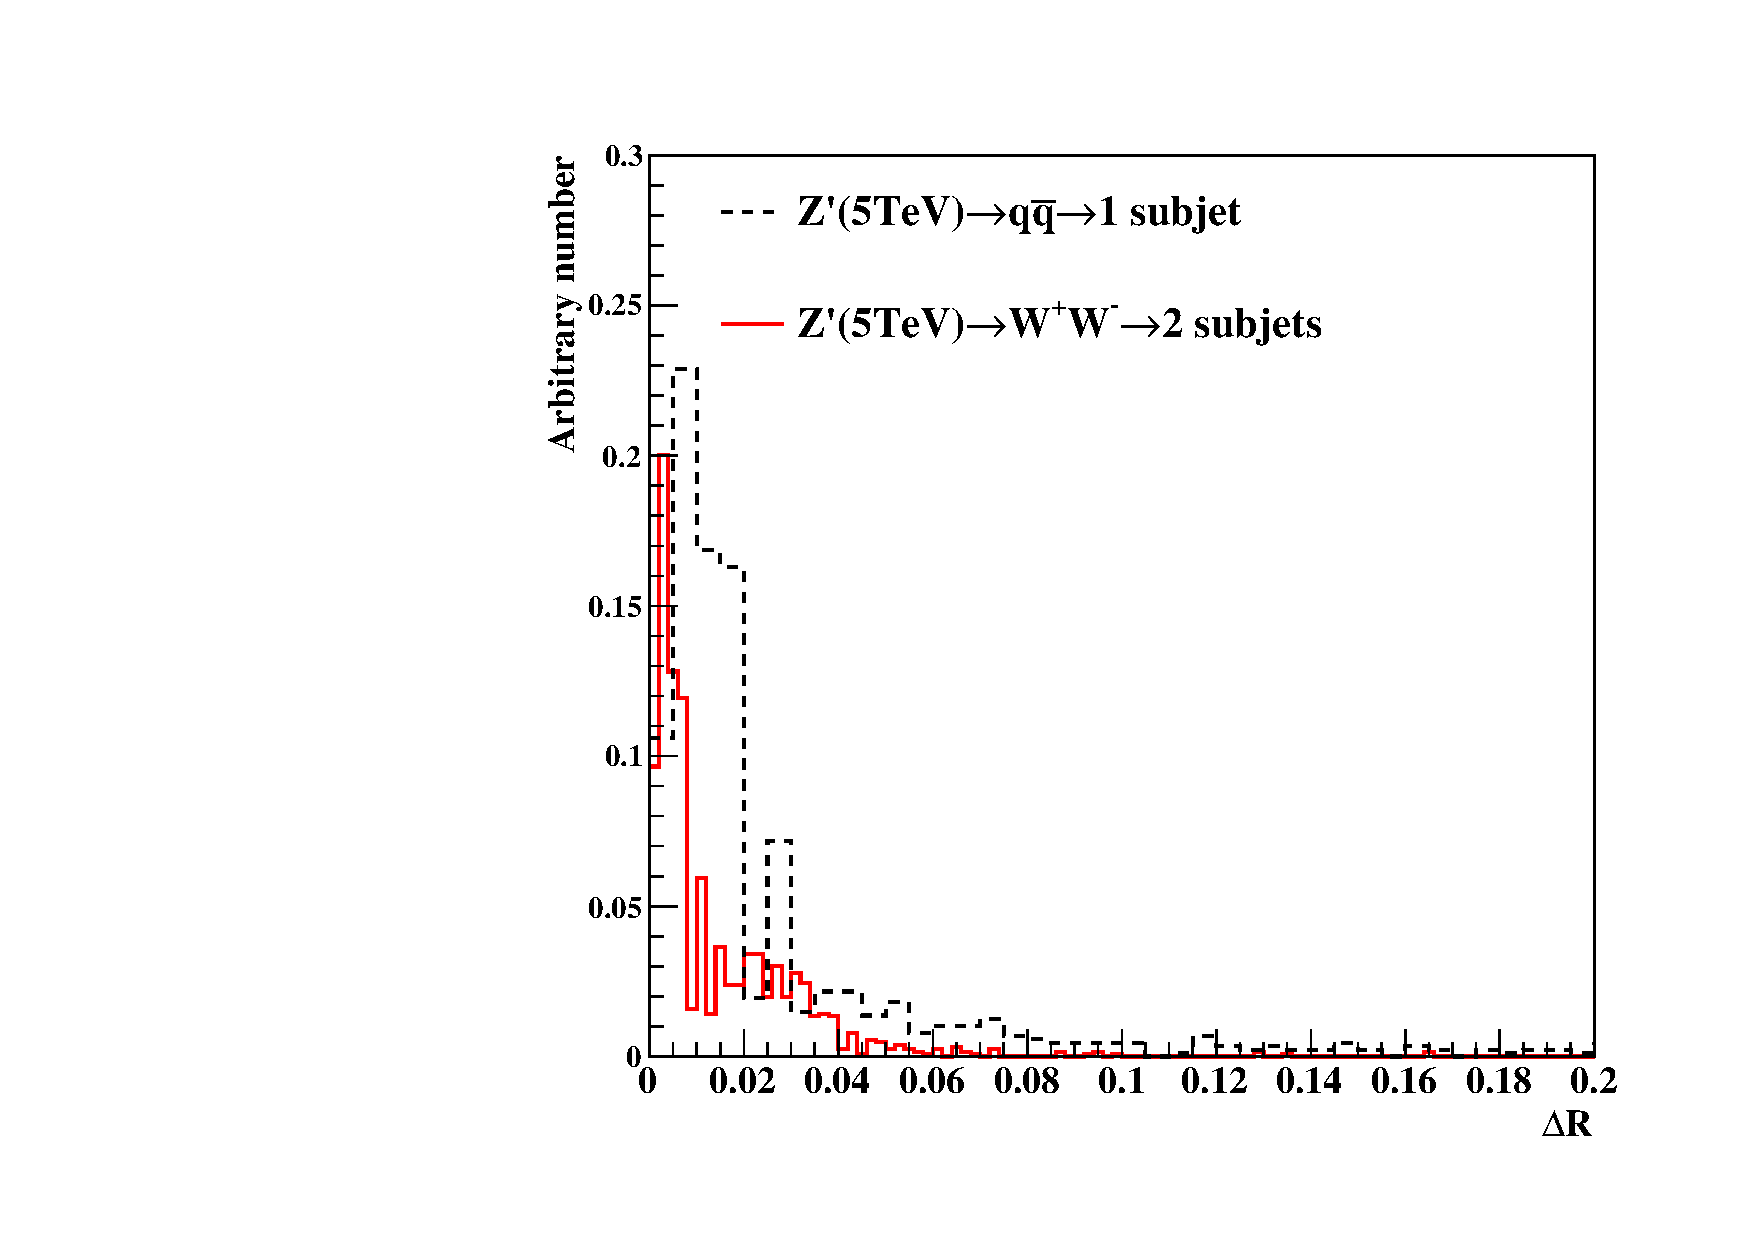
\includegraphics[width=0.3\textwidth]{/Users/ms08962476/Timing_paper/Pictures_used_for_FCC_and_jets/Reco_dR_Dis_ECAL/5TeV_Reco/dR_T_4_5TeV_Reco.pdf}
   }
\end{center}
\caption{Distributions of $\Delta R$ for $M(Z') = 5$~TeV for five kinds of trailing-T particles with the reco-level information of ECAL
are shown here.\label{fig:Reco_dR_Dis_5TeV_T}}
\end{figure}

\begin{figure}
\begin{center}
   \subfigure[The first trailing-PT] {
   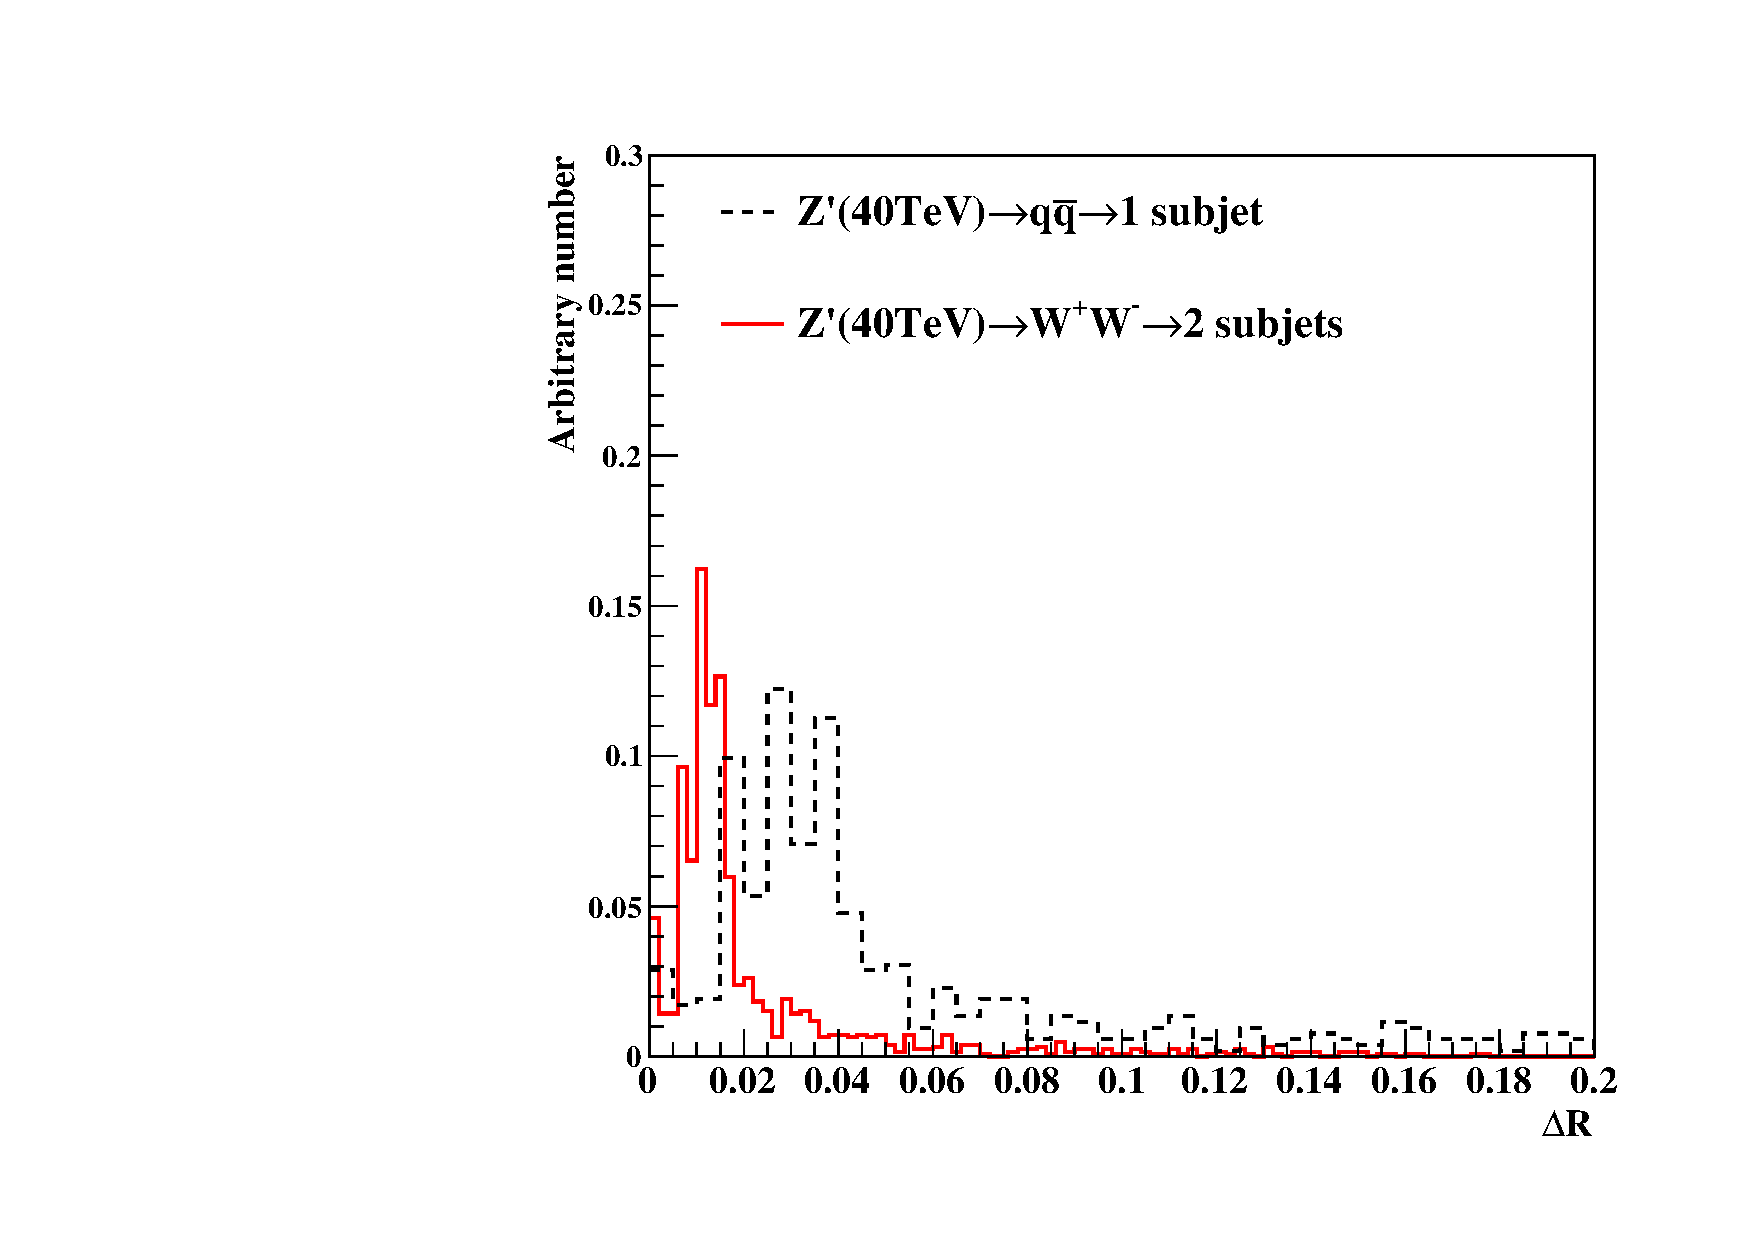
\includegraphics[width=0.3\textwidth]{/Users/ms08962476/Timing_paper/Pictures_used_for_FCC_and_jets/Reco_dR_Dis_ECAL/40TeV_Reco/dR_PT_0_40TeV_Reco.pdf}
   }
   \subfigure[The second trailing-PT] {
   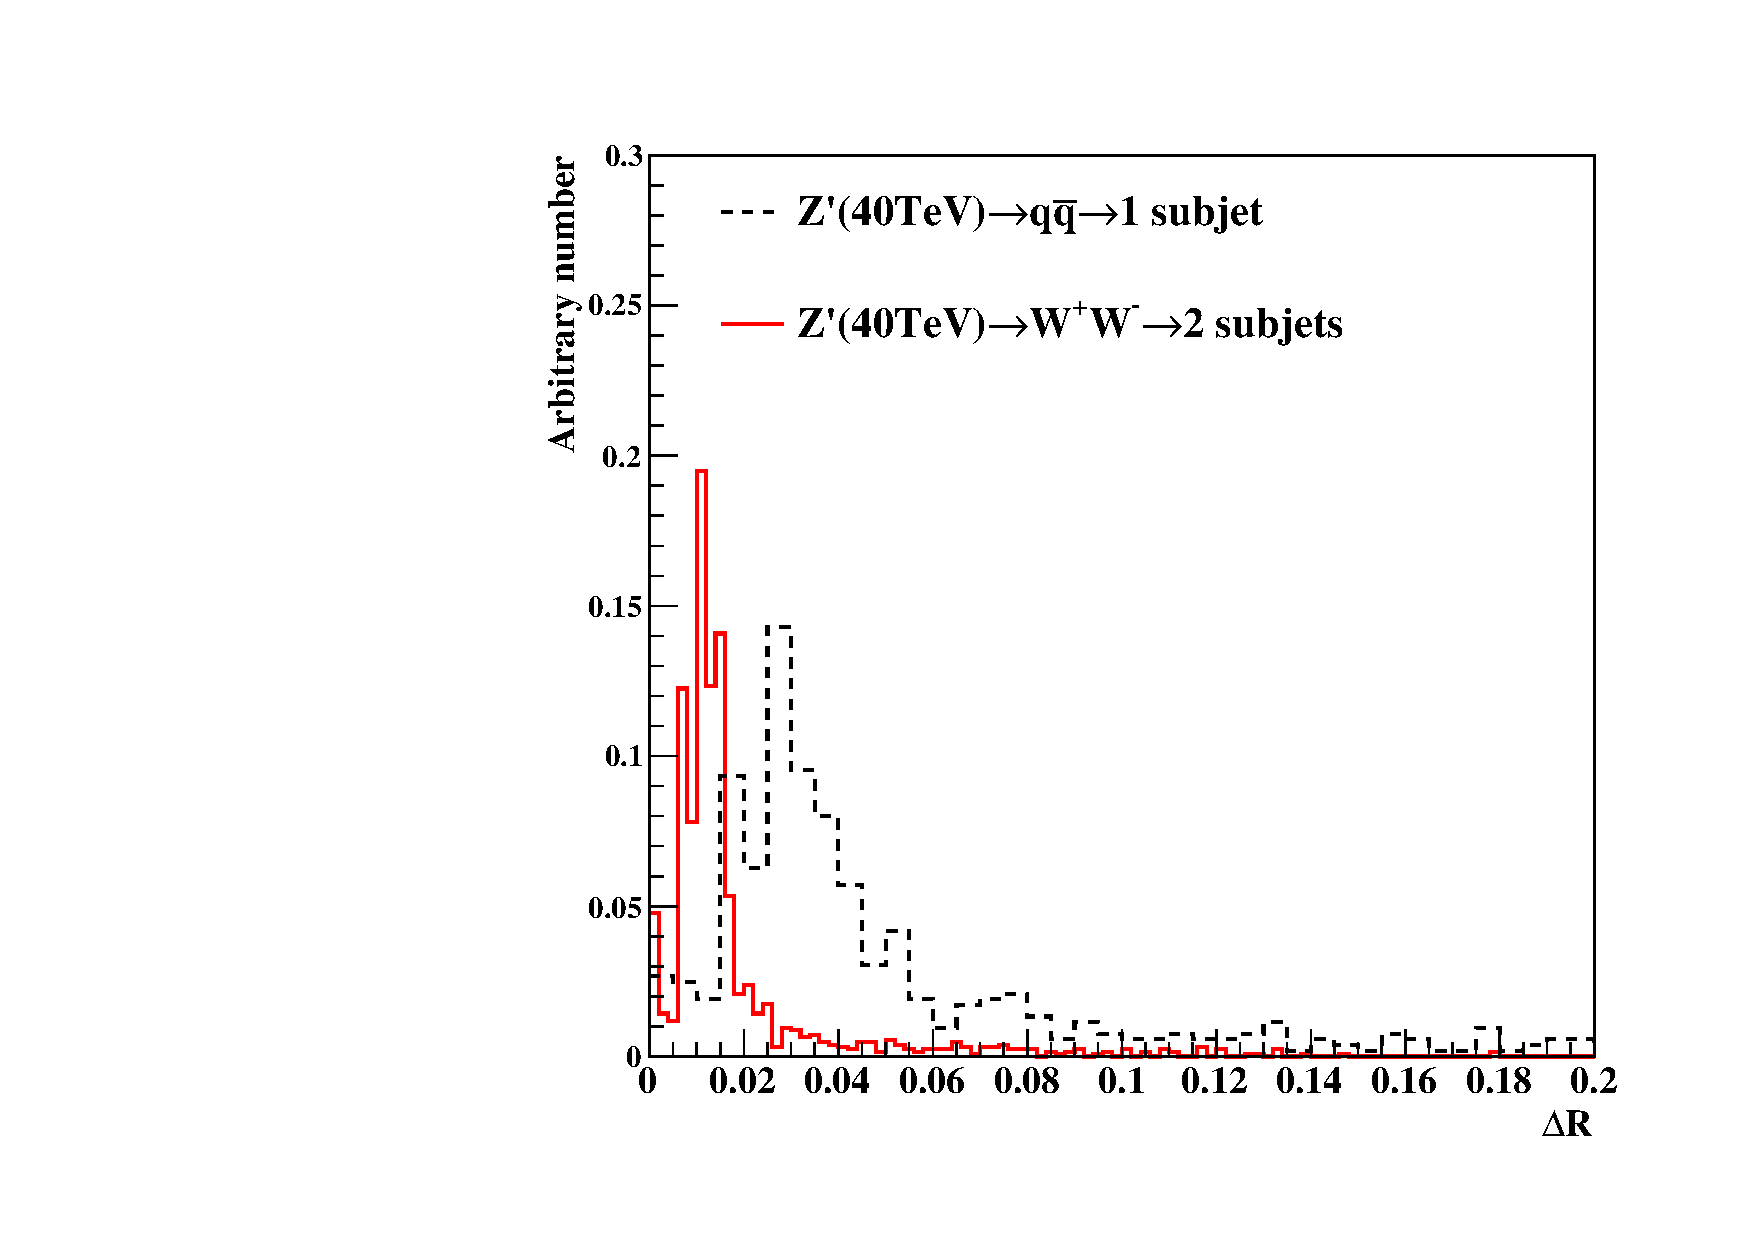
\includegraphics[width=0.3\textwidth]{/Users/ms08962476/Timing_paper/Pictures_used_for_FCC_and_jets/Reco_dR_Dis_ECAL/40TeV_Reco/dR_PT_1_40TeV_Reco.pdf}
   }
   \subfigure[The third trailing-PT] {
   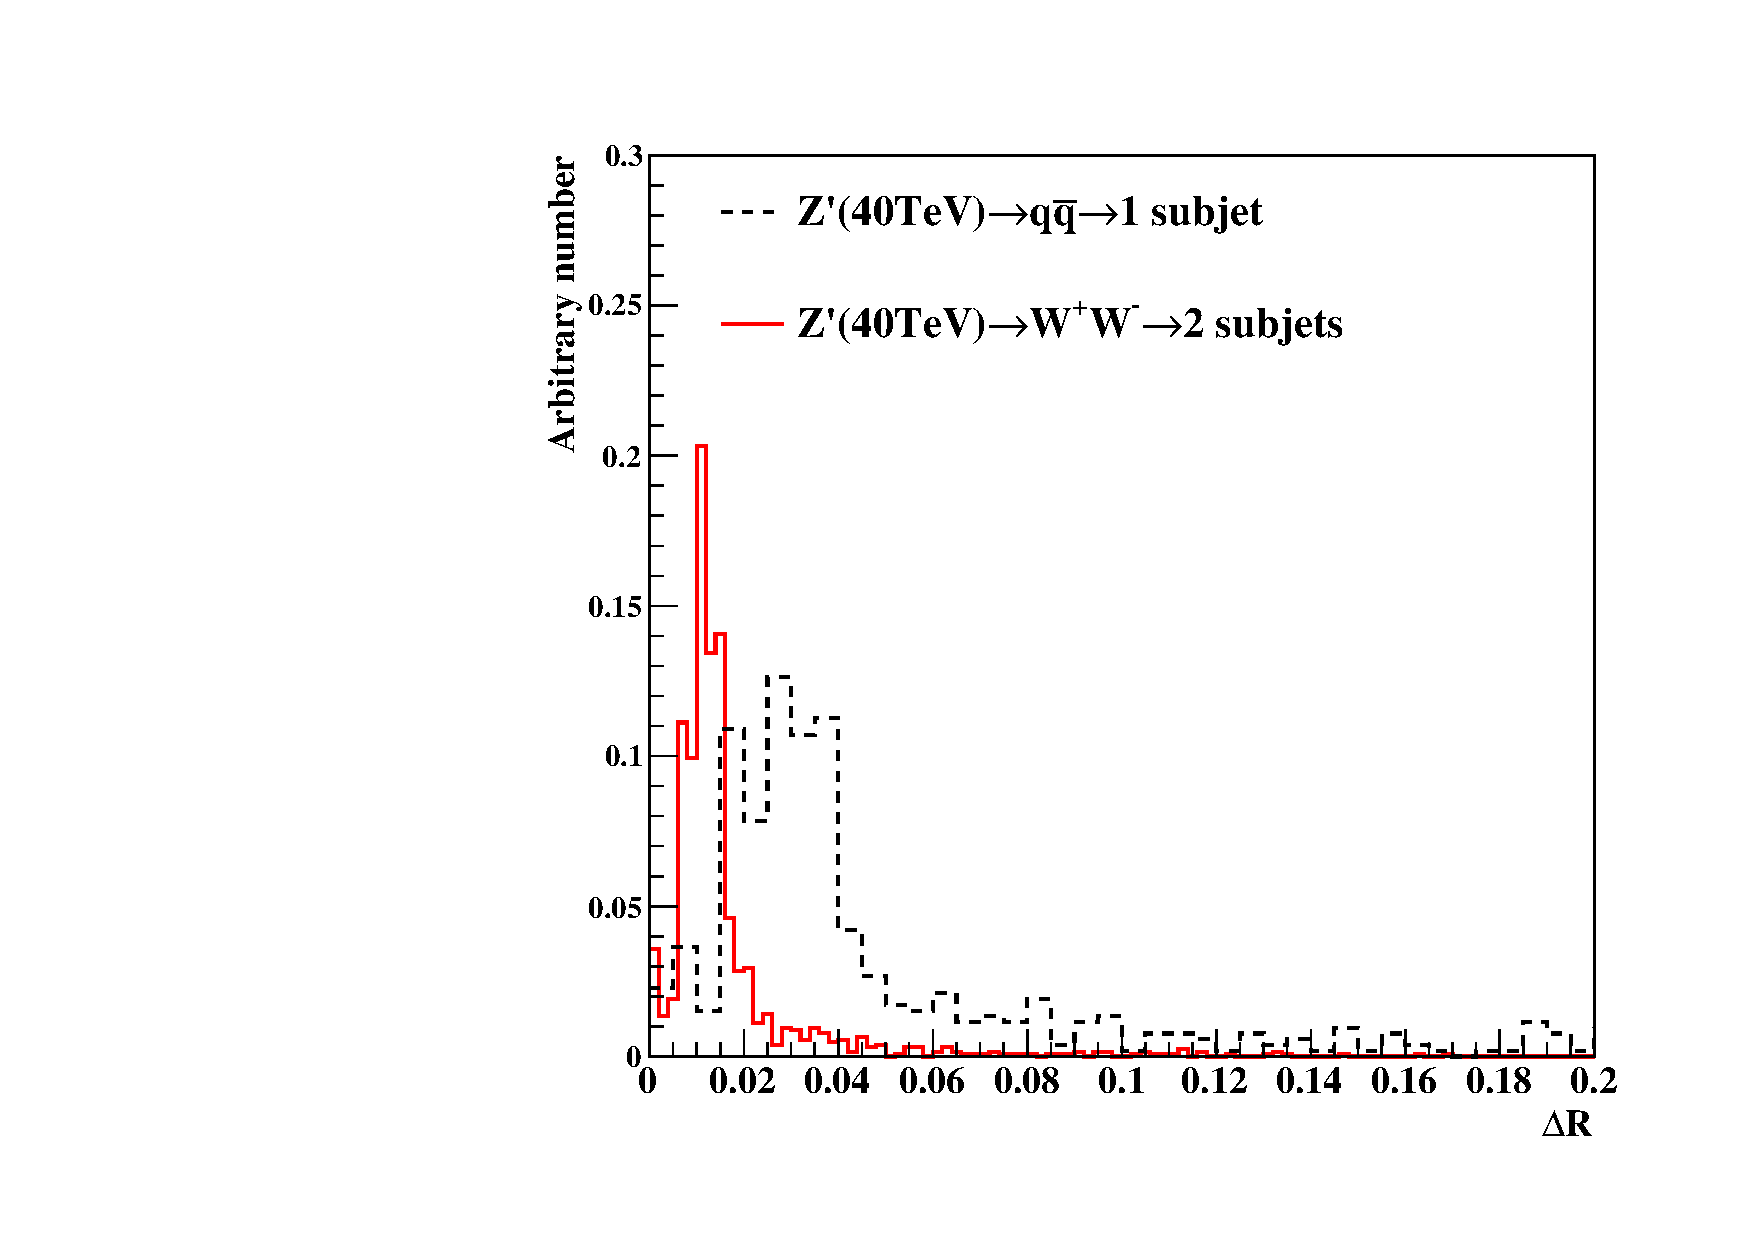
\includegraphics[width=0.3\textwidth]{/Users/ms08962476/Timing_paper/Pictures_used_for_FCC_and_jets/Reco_dR_Dis_ECAL/40TeV_Reco/dR_PT_2_40TeV_Reco.pdf}
   }
      \subfigure[The fourth trailing-PT] {
   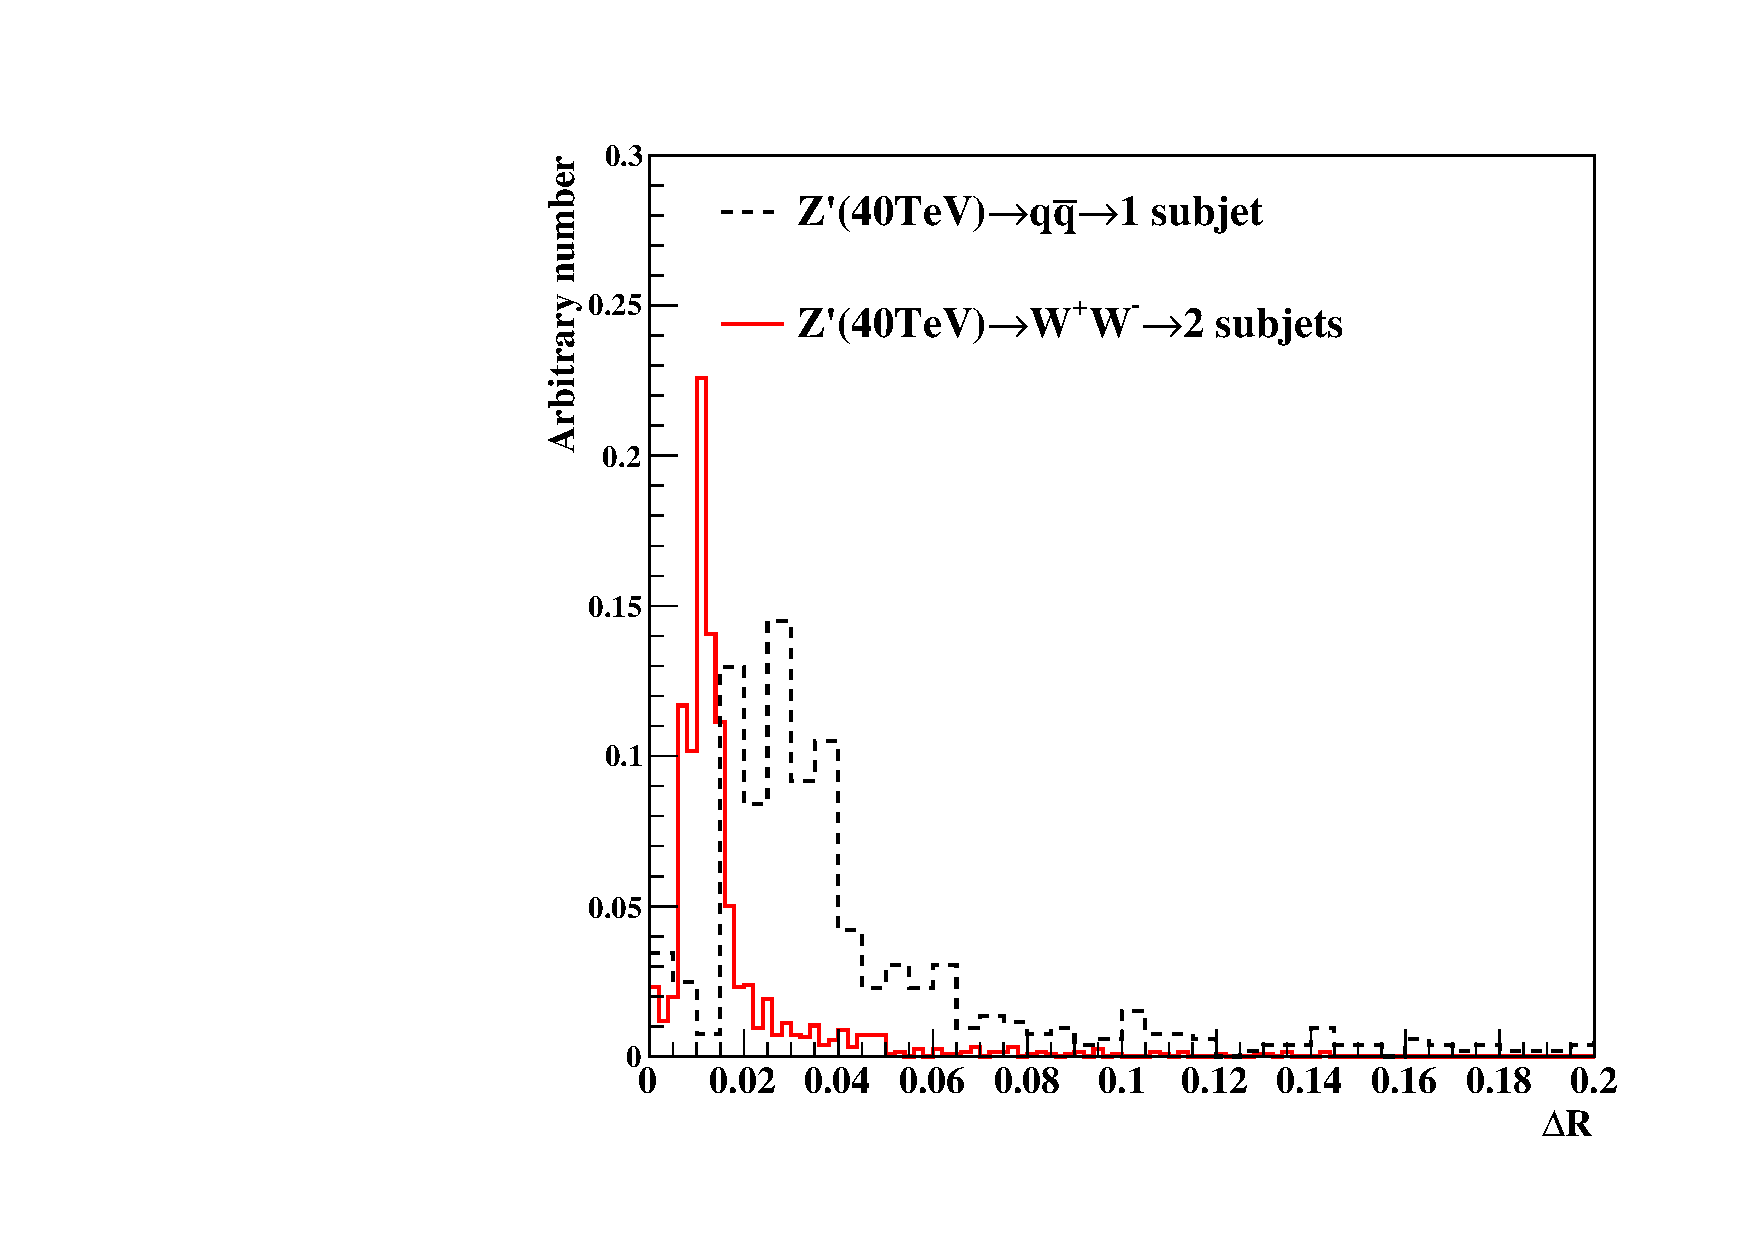
\includegraphics[width=0.3\textwidth]{/Users/ms08962476/Timing_paper/Pictures_used_for_FCC_and_jets/Reco_dR_Dis_ECAL/40TeV_Reco/dR_PT_3_40TeV_Reco.pdf}
   }
   \subfigure[The fifth trailing-PT] {
   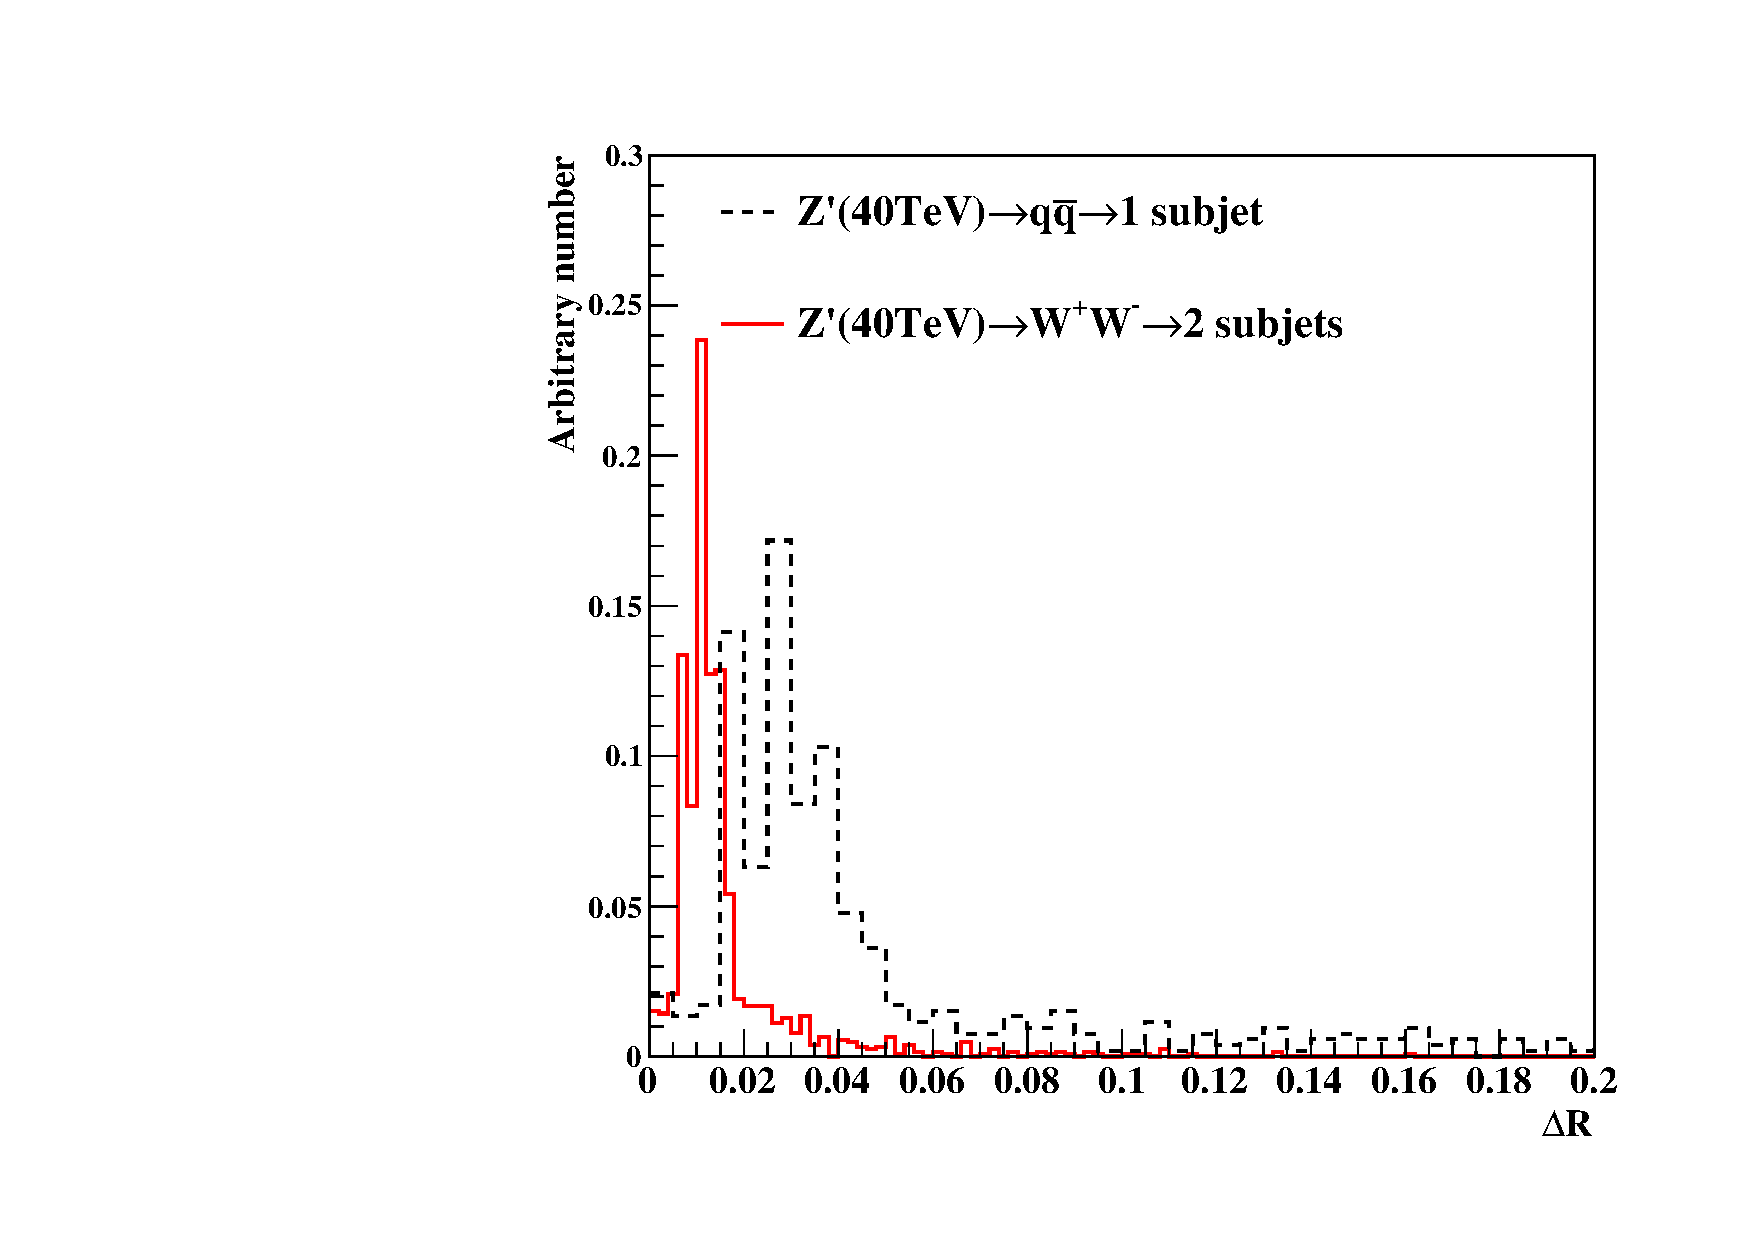
\includegraphics[width=0.3\textwidth]{/Users/ms08962476/Timing_paper/Pictures_used_for_FCC_and_jets/Reco_dR_Dis_ECAL/40TeV_Reco/dR_PT_4_40TeV_Reco.pdf}
   }
\end{center}
\caption{Distributions of $\Delta R$ for $M(Z') = 40$~TeV for five kinds of trailing-$P_{T}$ particles with the reco-level information of ECAL
are shown here. \label{fig:Reco_dR_Dis_40TeV_PT}}
\end{figure}

\begin{figure}
\begin{center}
   \subfigure[The first trailing-T] {
   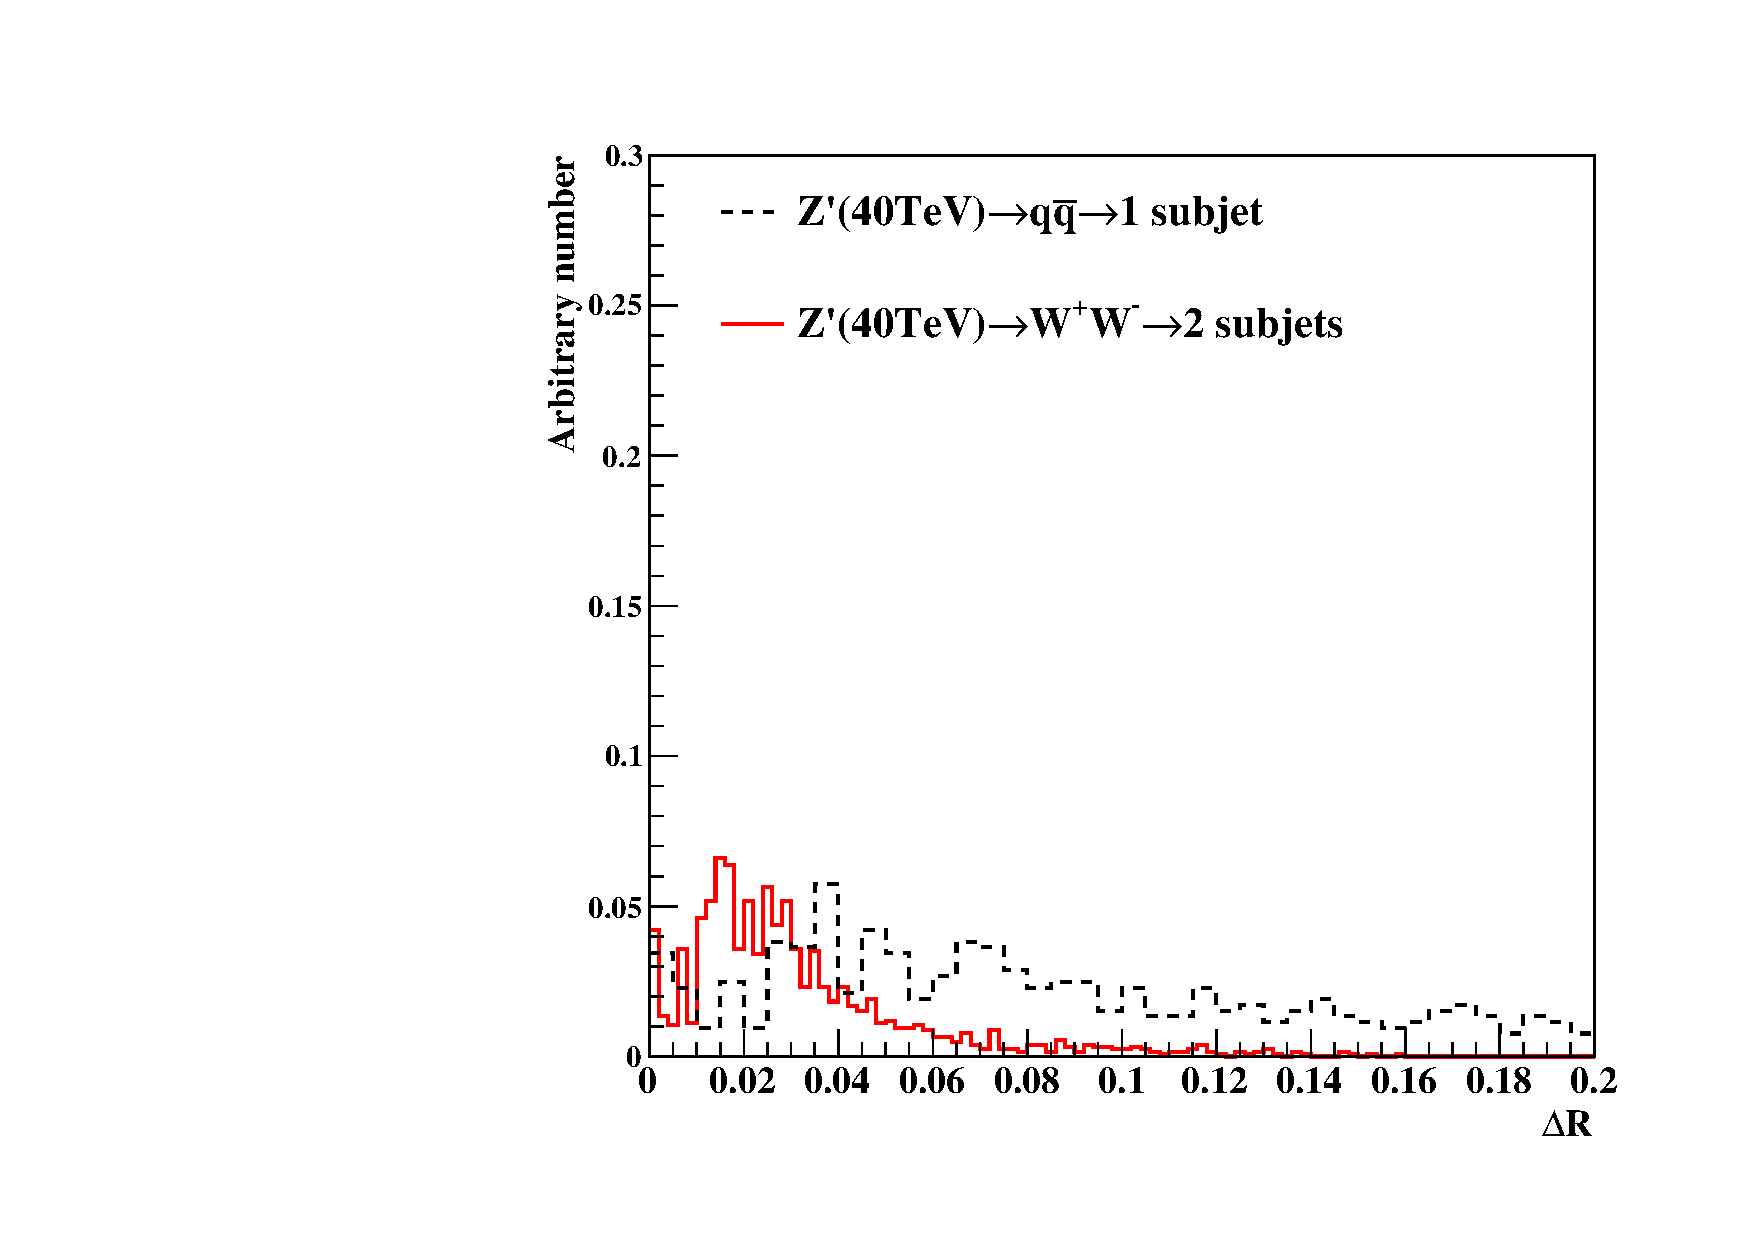
\includegraphics[width=0.3\textwidth]{/Users/ms08962476/Timing_paper/Pictures_used_for_FCC_and_jets/Reco_dR_Dis_ECAL/40TeV_Reco/dR_T_0_40TeV_Reco.pdf}
   }
   \subfigure[The second trailing-T] {
   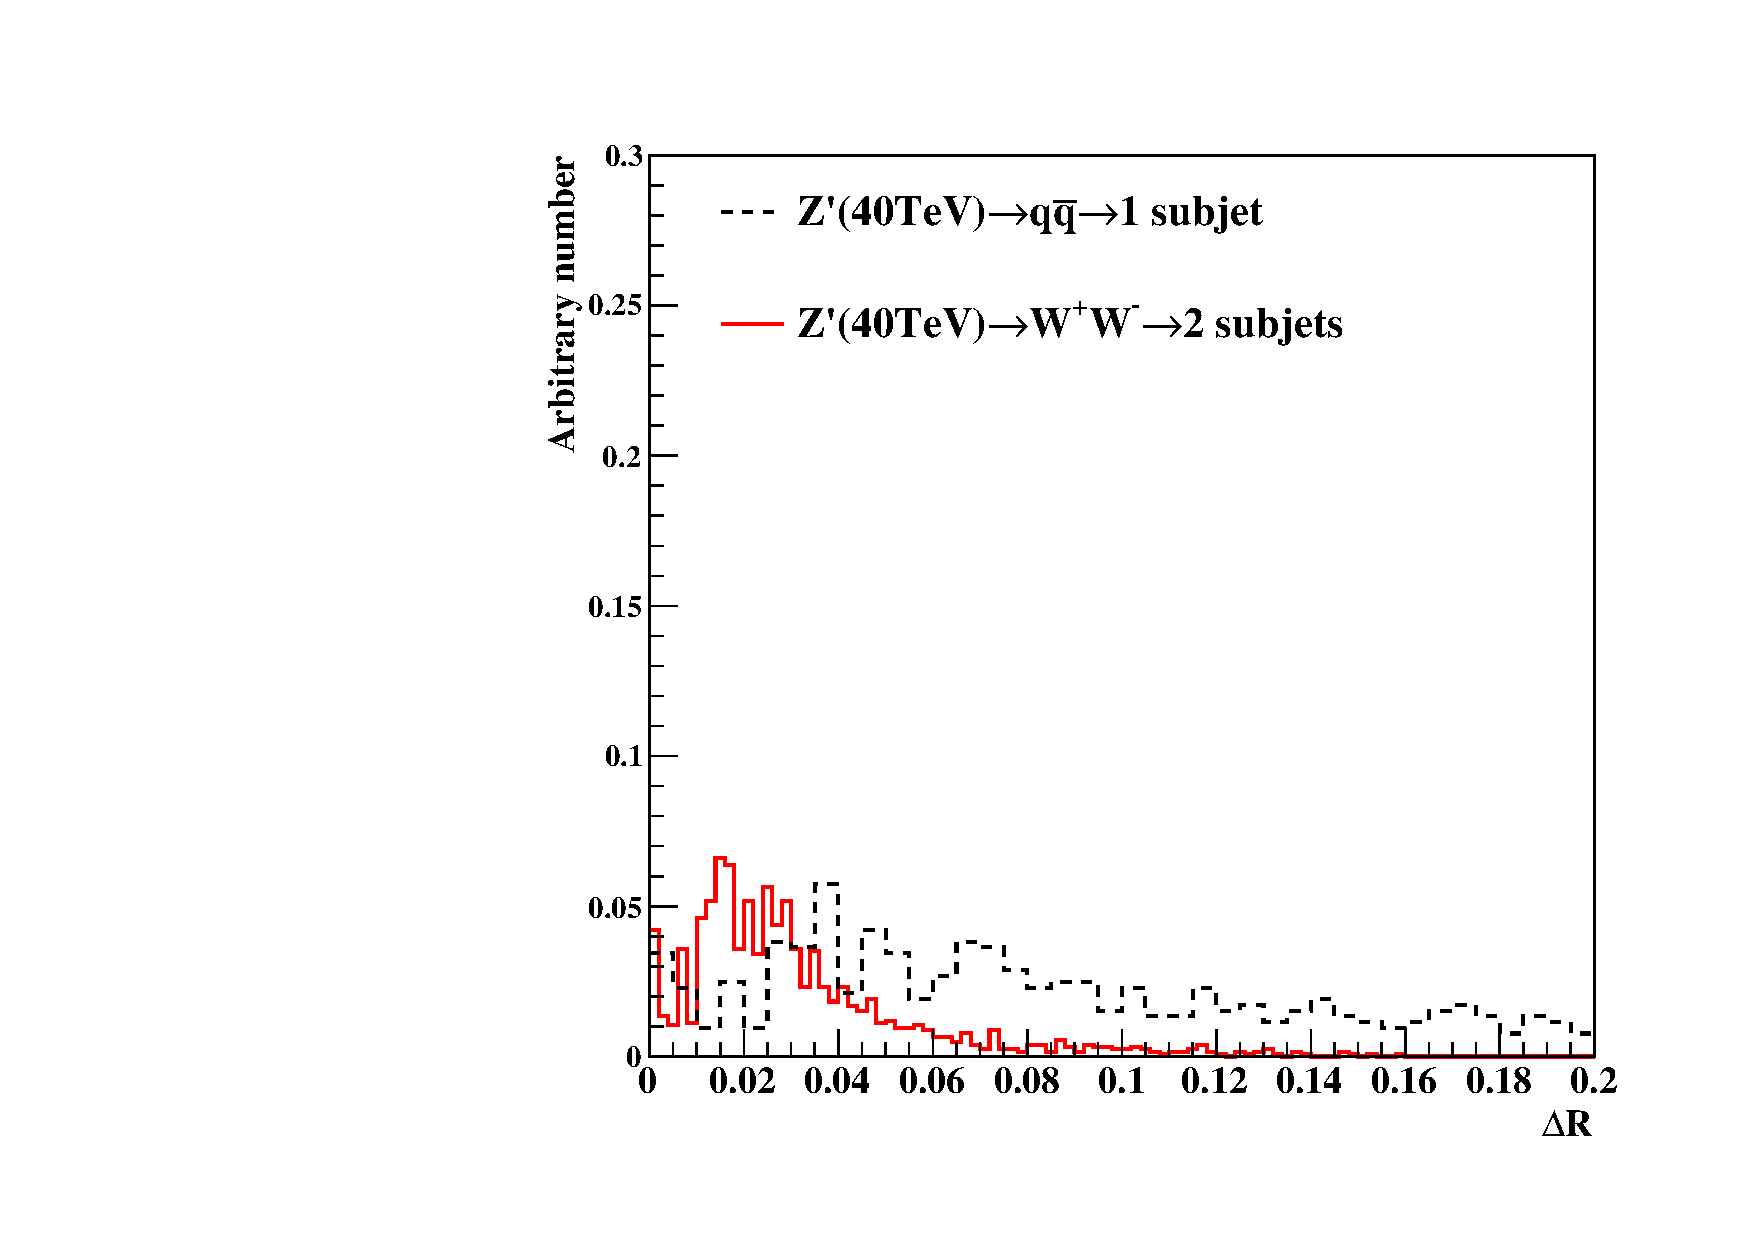
\includegraphics[width=0.3\textwidth]{/Users/ms08962476/Timing_paper/Pictures_used_for_FCC_and_jets/Reco_dR_Dis_ECAL/40TeV_Reco/dR_T_1_40TeV_Reco.pdf}
   }
   \subfigure[The third trailing-T] {
   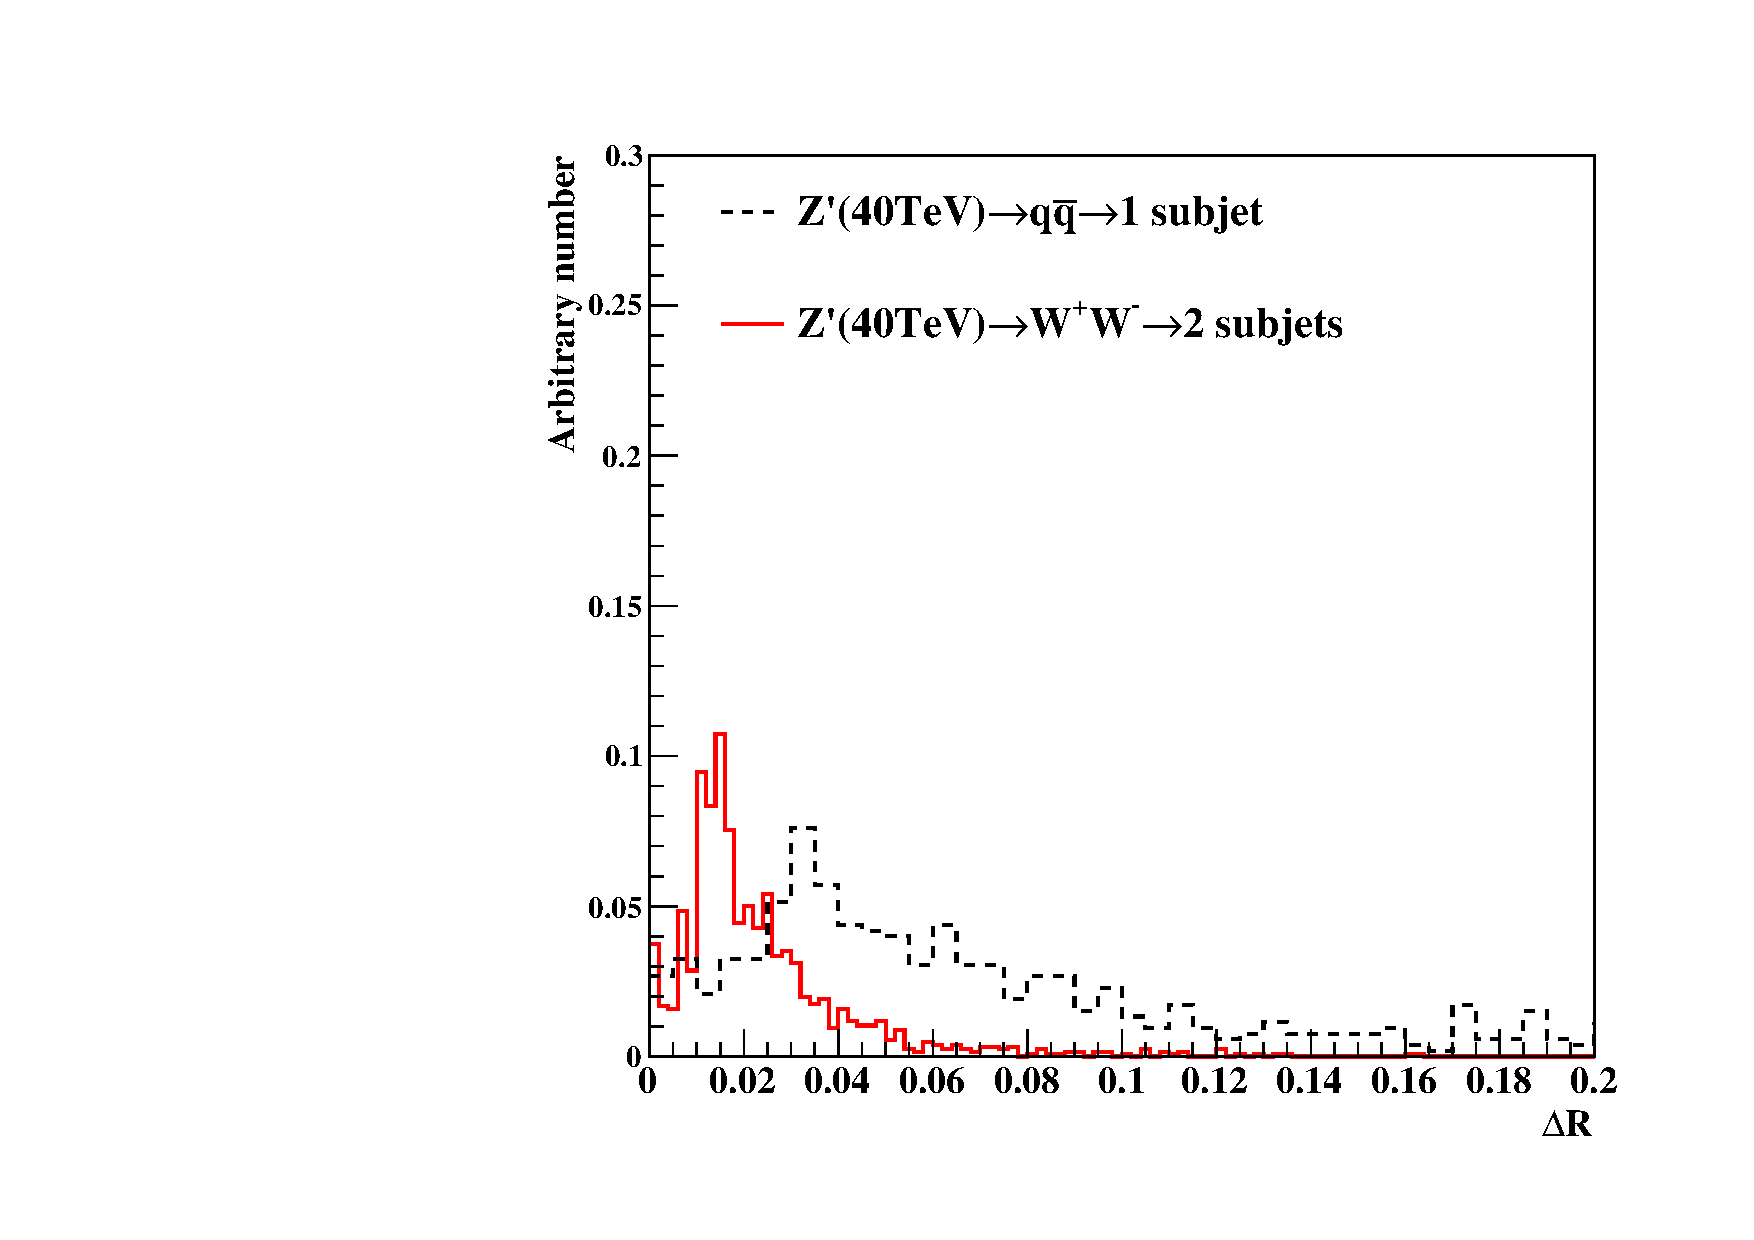
\includegraphics[width=0.3\textwidth]{/Users/ms08962476/Timing_paper/Pictures_used_for_FCC_and_jets/Reco_dR_Dis_ECAL/40TeV_Reco/dR_T_2_40TeV_Reco.pdf}
   }
      \subfigure[The fourth trailing-T] {
   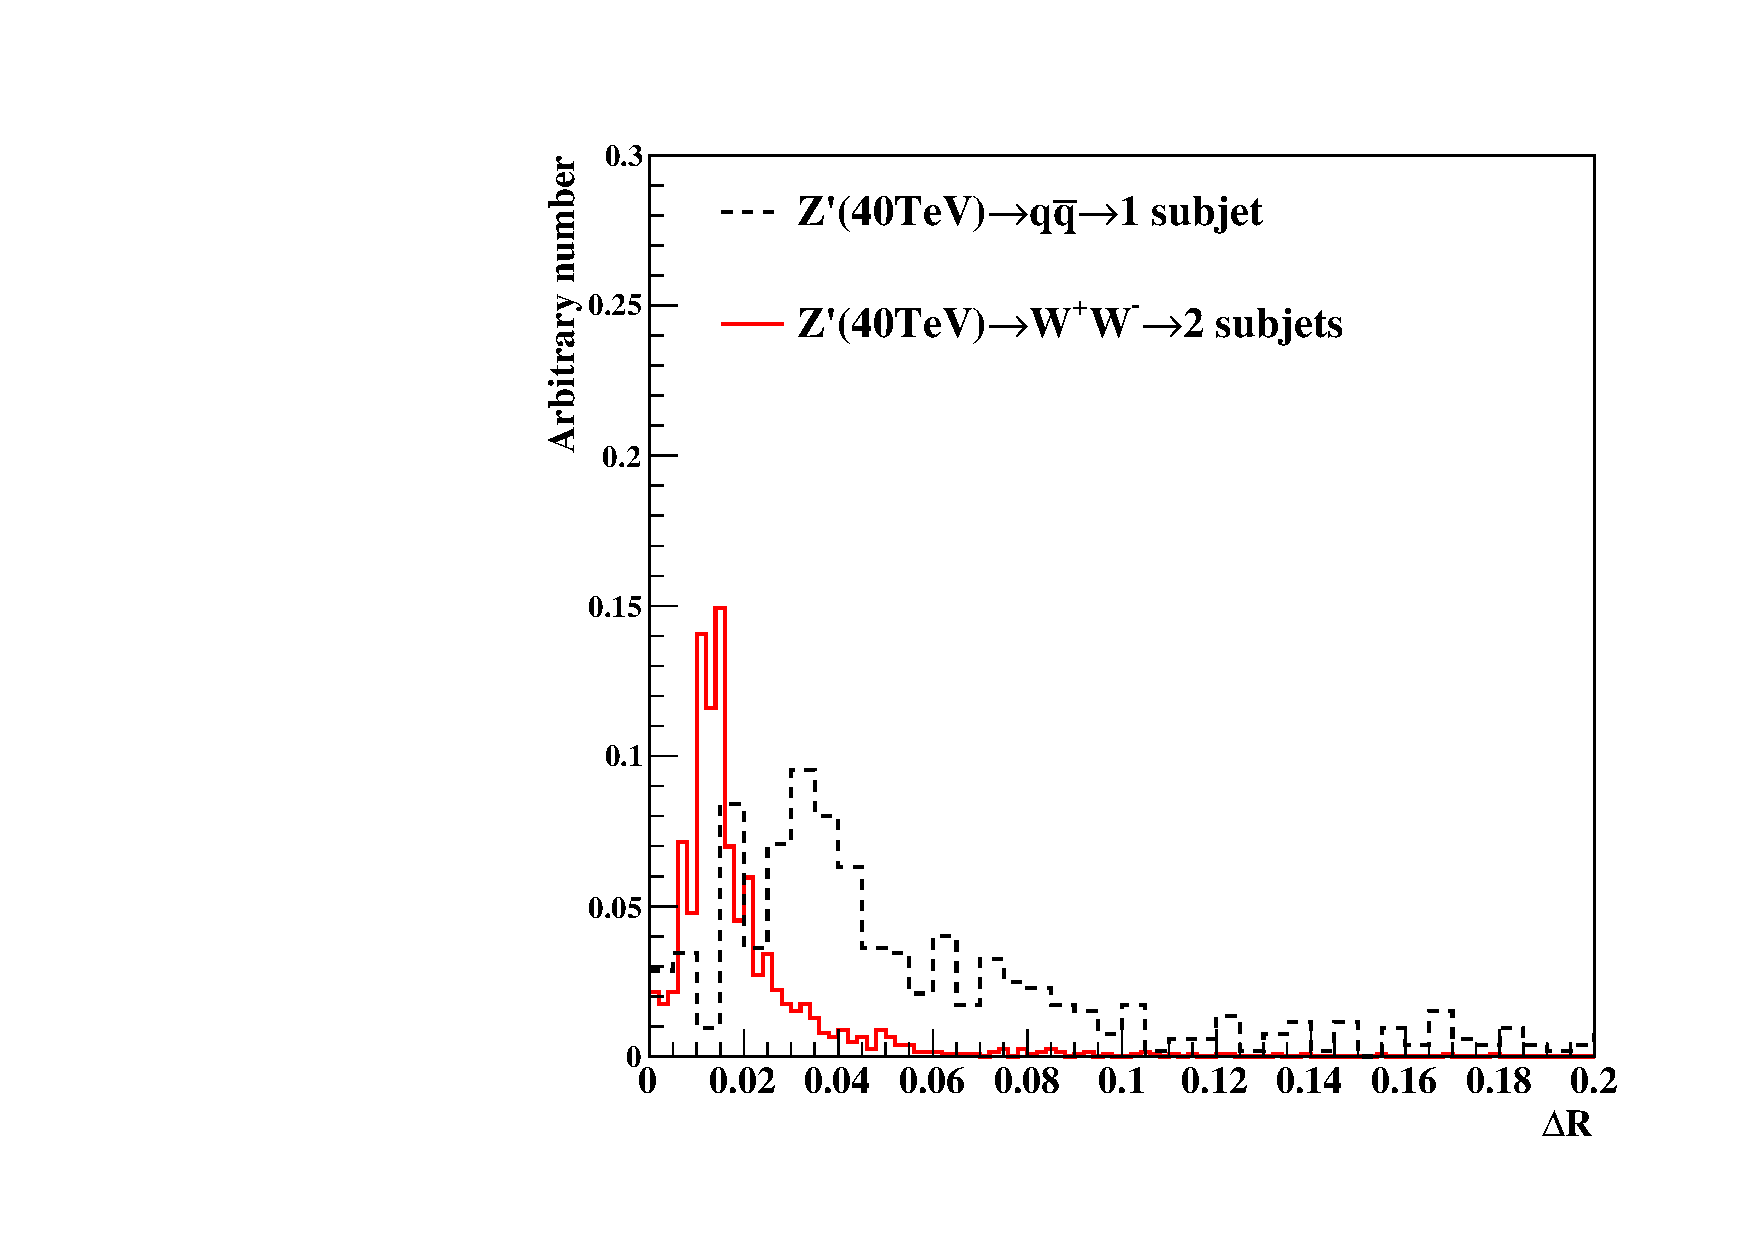
\includegraphics[width=0.3\textwidth]{/Users/ms08962476/Timing_paper/Pictures_used_for_FCC_and_jets/Reco_dR_Dis_ECAL/40TeV_Reco/dR_T_3_40TeV_Reco.pdf}
   }
   \subfigure[The fifth trailing-T] {
   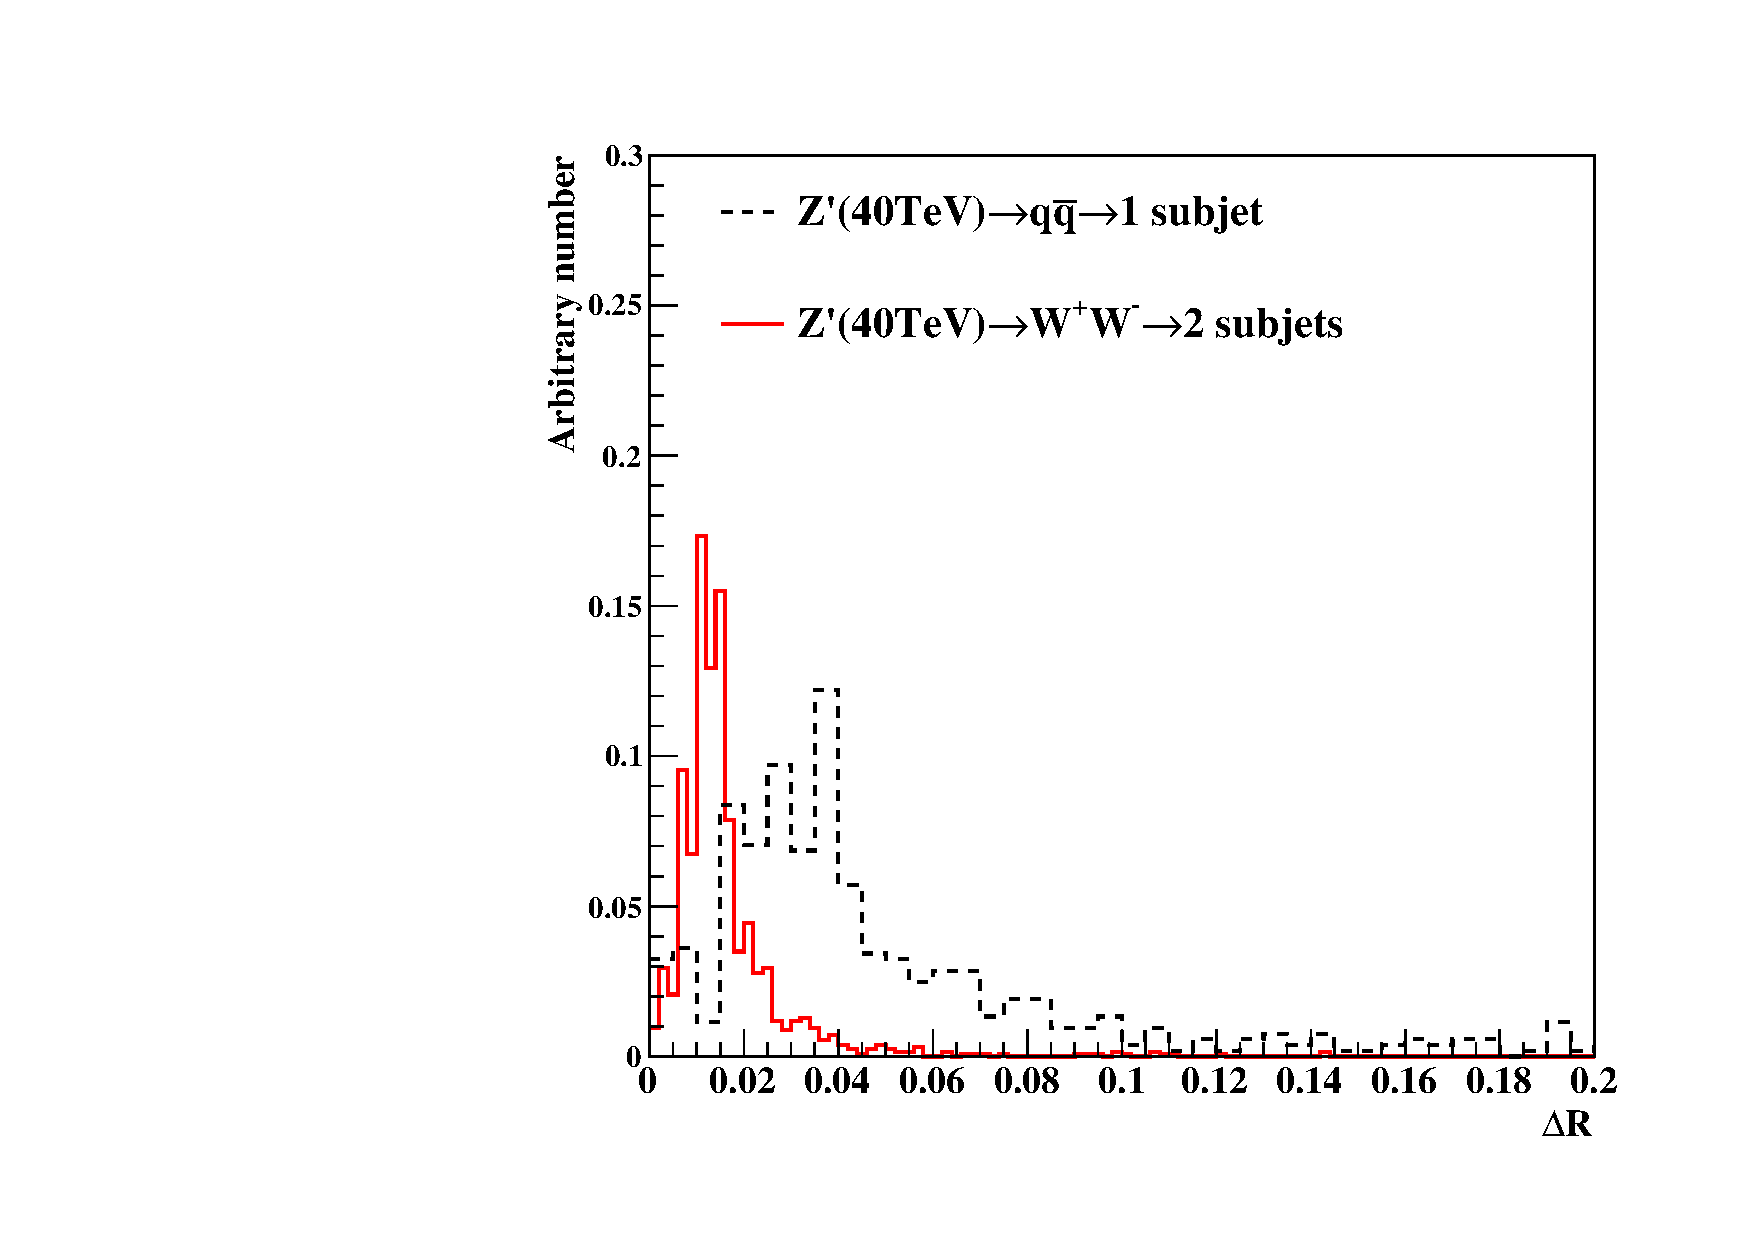
\includegraphics[width=0.3\textwidth]{/Users/ms08962476/Timing_paper/Pictures_used_for_FCC_and_jets/Reco_dR_Dis_ECAL/40TeV_Reco/dR_T_4_40TeV_Reco.pdf}
   }
\end{center}
\caption{Distributions of $\Delta R$ for $M(Z') = 40$~TeV for five kinds of trailing-T particles with the reco-level information of ECAL
are shown here. \label{fig:Reco_dR_Dis_40TeV_T}}
\end{figure}

\begin{figure}
\begin{center}
   \subfigure[5TeV] {
   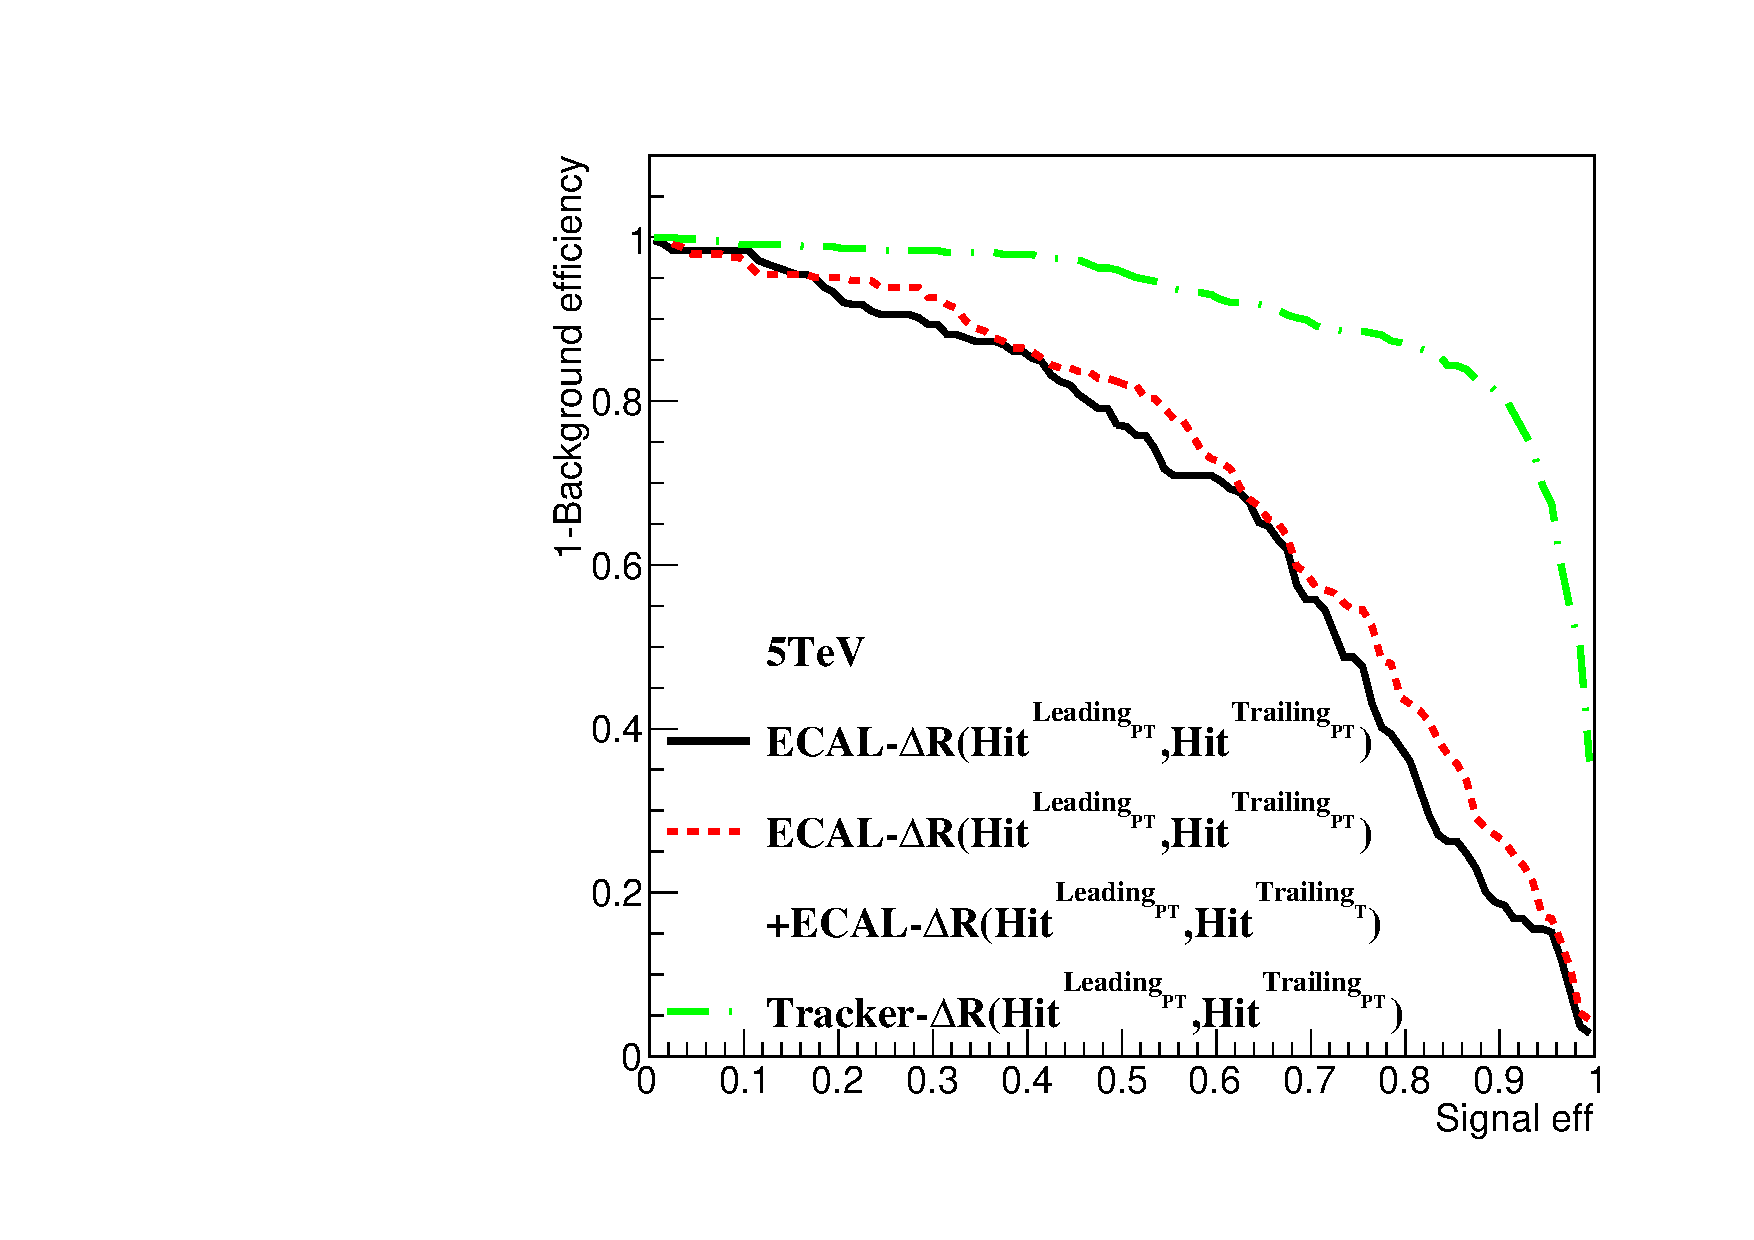
\includegraphics[width=0.4\textwidth]{/Users/ms08962476/Timing_paper/Pictures_used_for_FCC_and_jets/Reco_dR_BDT/BDT_plot_dR_dRplusID_5TeV_Reco.pdf}
   }
   \subfigure[10TeV] {
   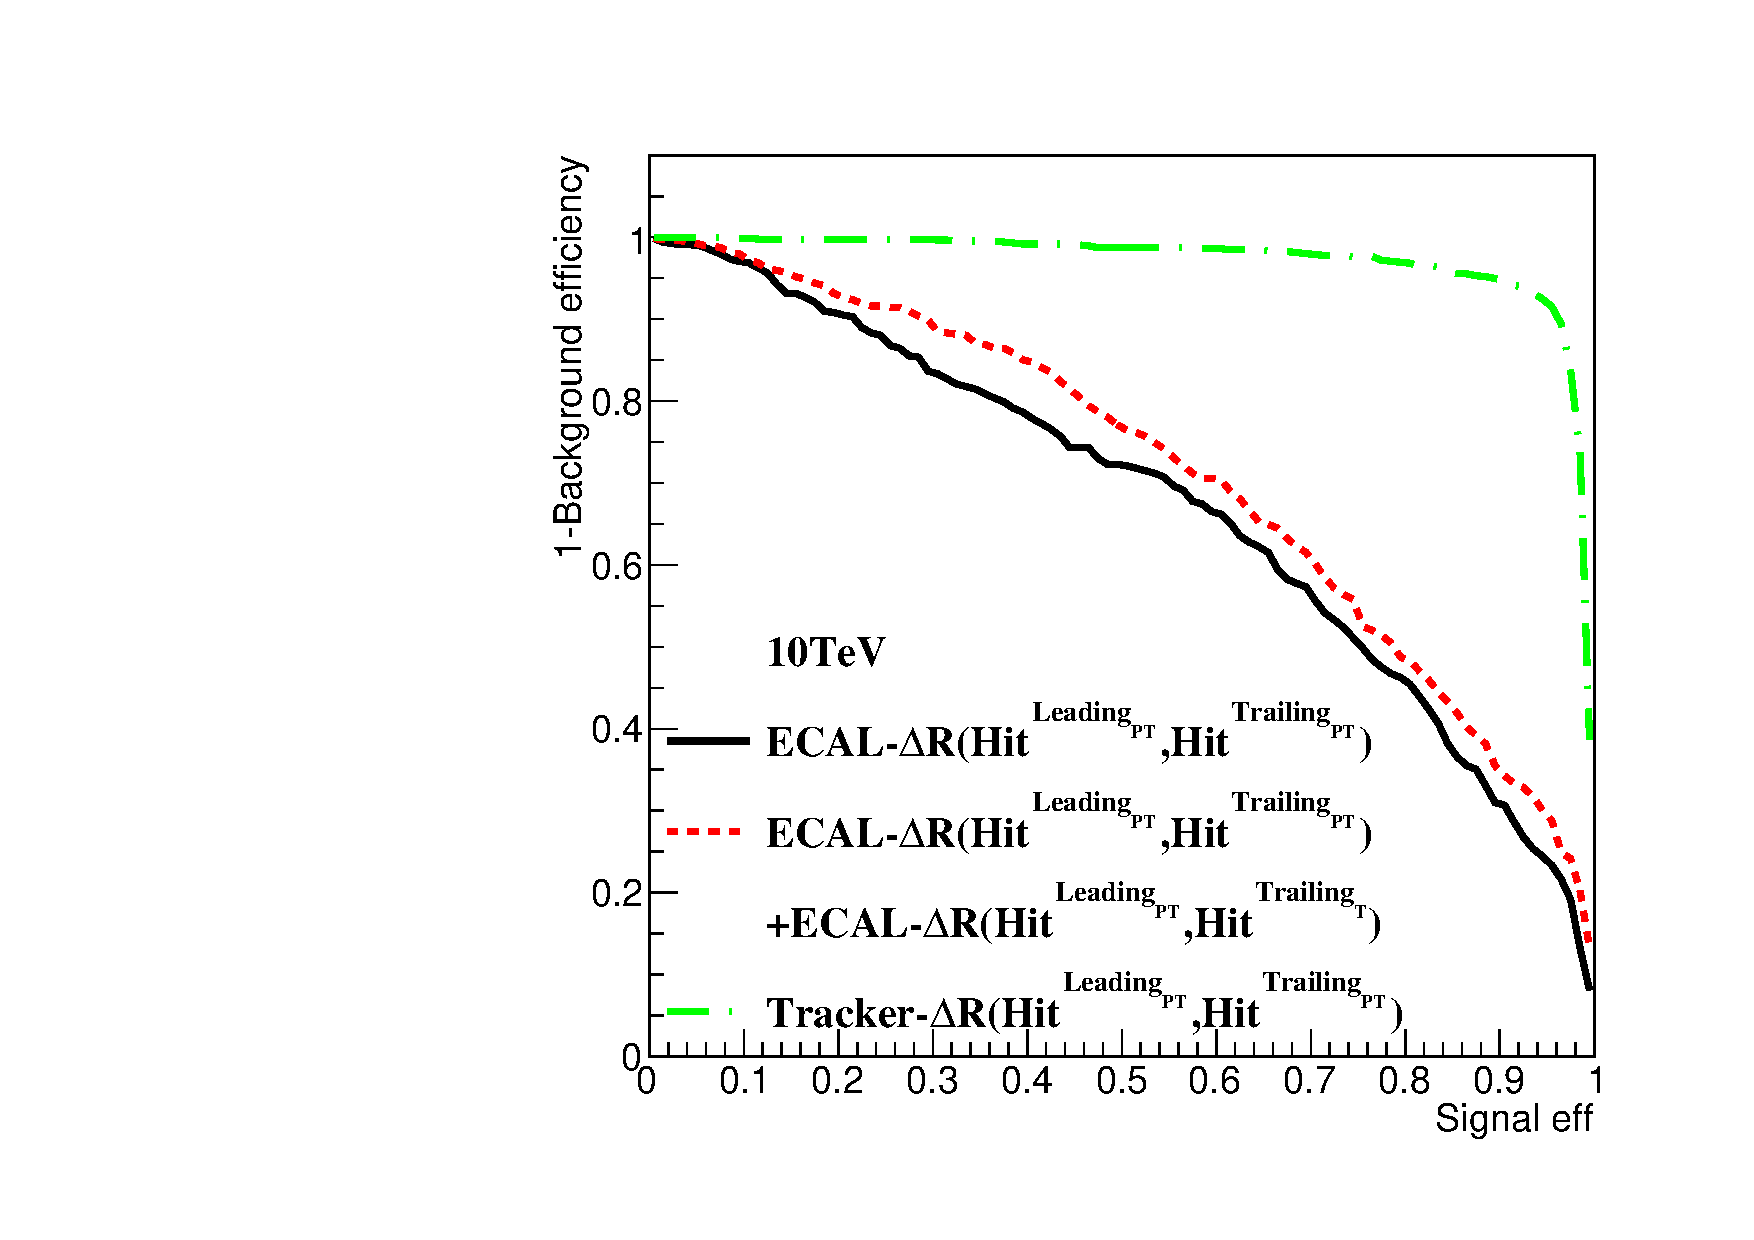
\includegraphics[width=0.4\textwidth]{/Users/ms08962476/Timing_paper/Pictures_used_for_FCC_and_jets/Reco_dR_BDT/BDT_plot_dR_dRplusID_10TeV_Reco.pdf}
   }
   \subfigure[20TeV] {
   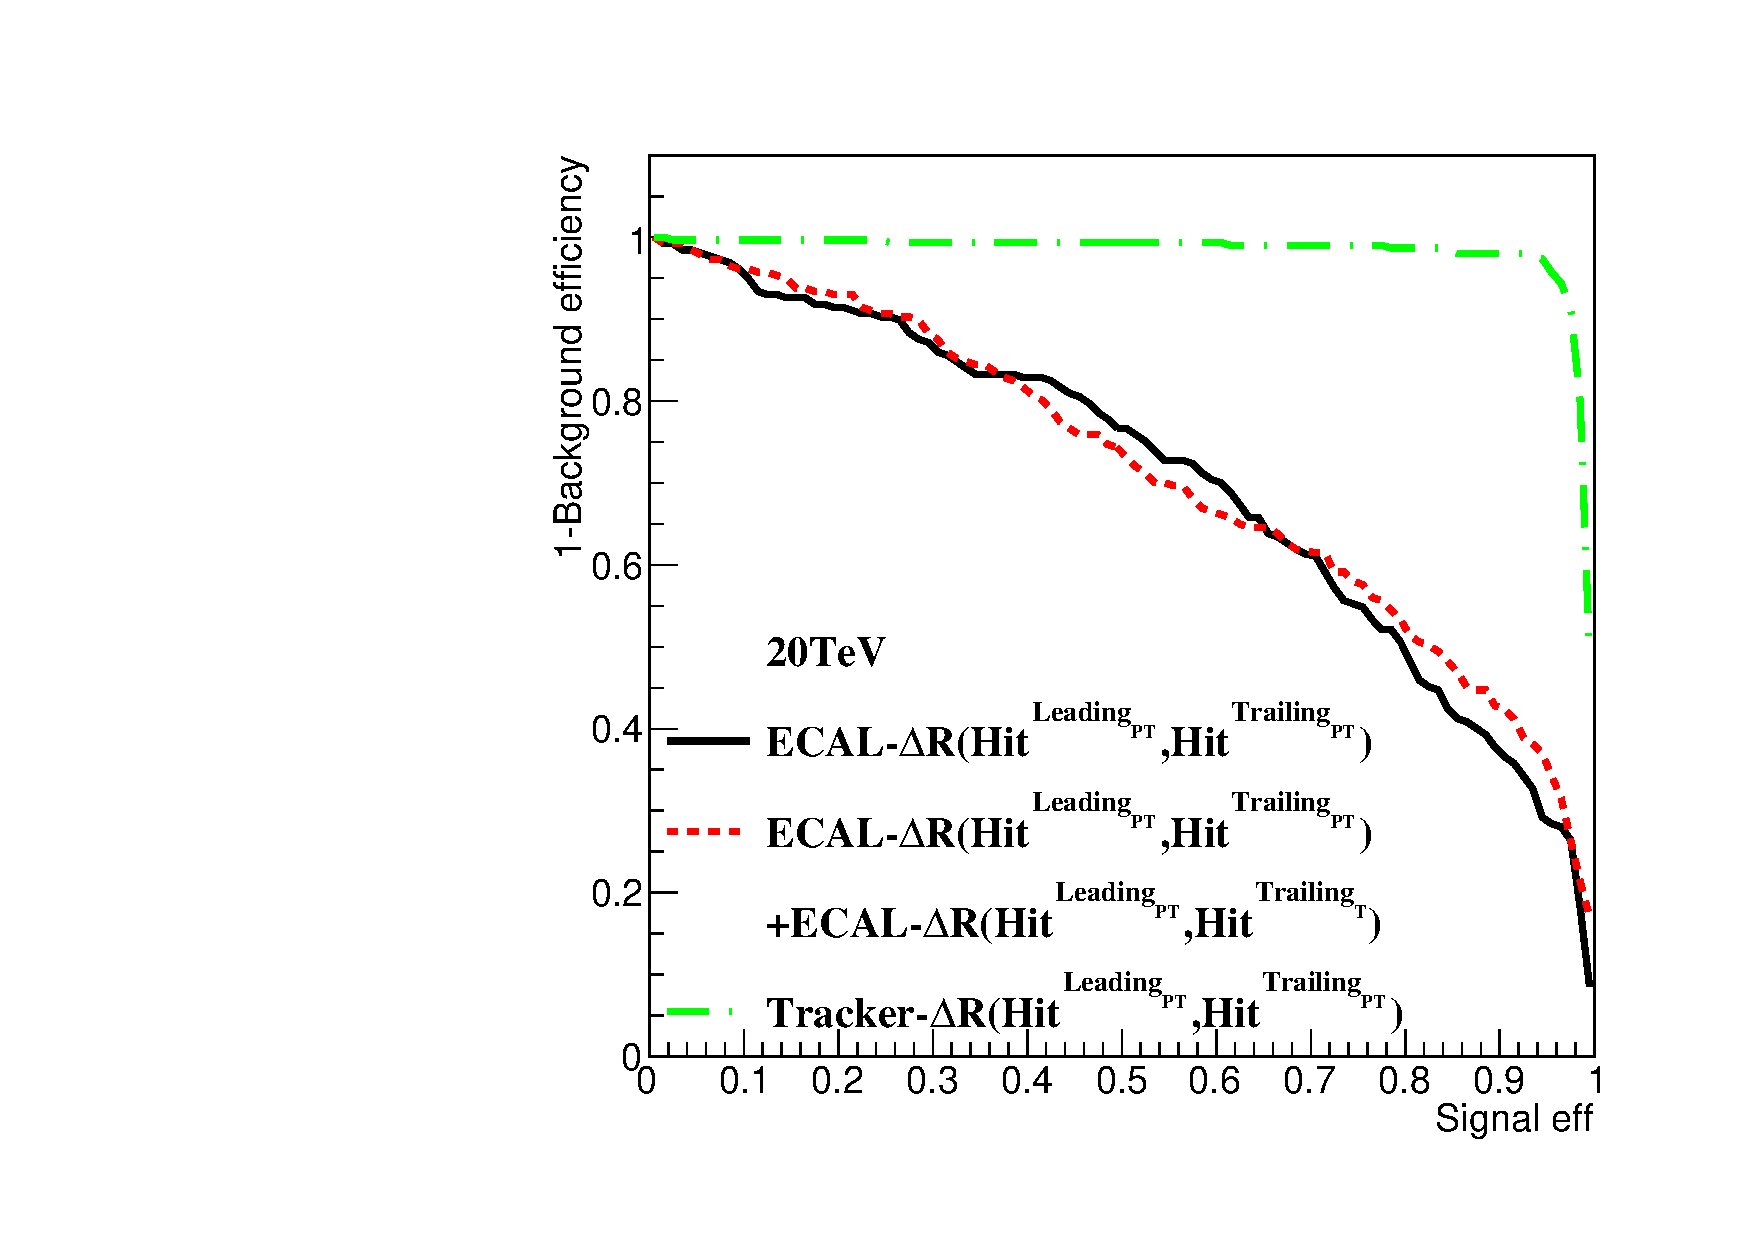
\includegraphics[width=0.4\textwidth]{/Users/ms08962476/Timing_paper/Pictures_used_for_FCC_and_jets/Reco_dR_BDT/BDT_plot_dR_dRplusID_20TeV_Reco.pdf}
   }
      \subfigure[40TeV] {
   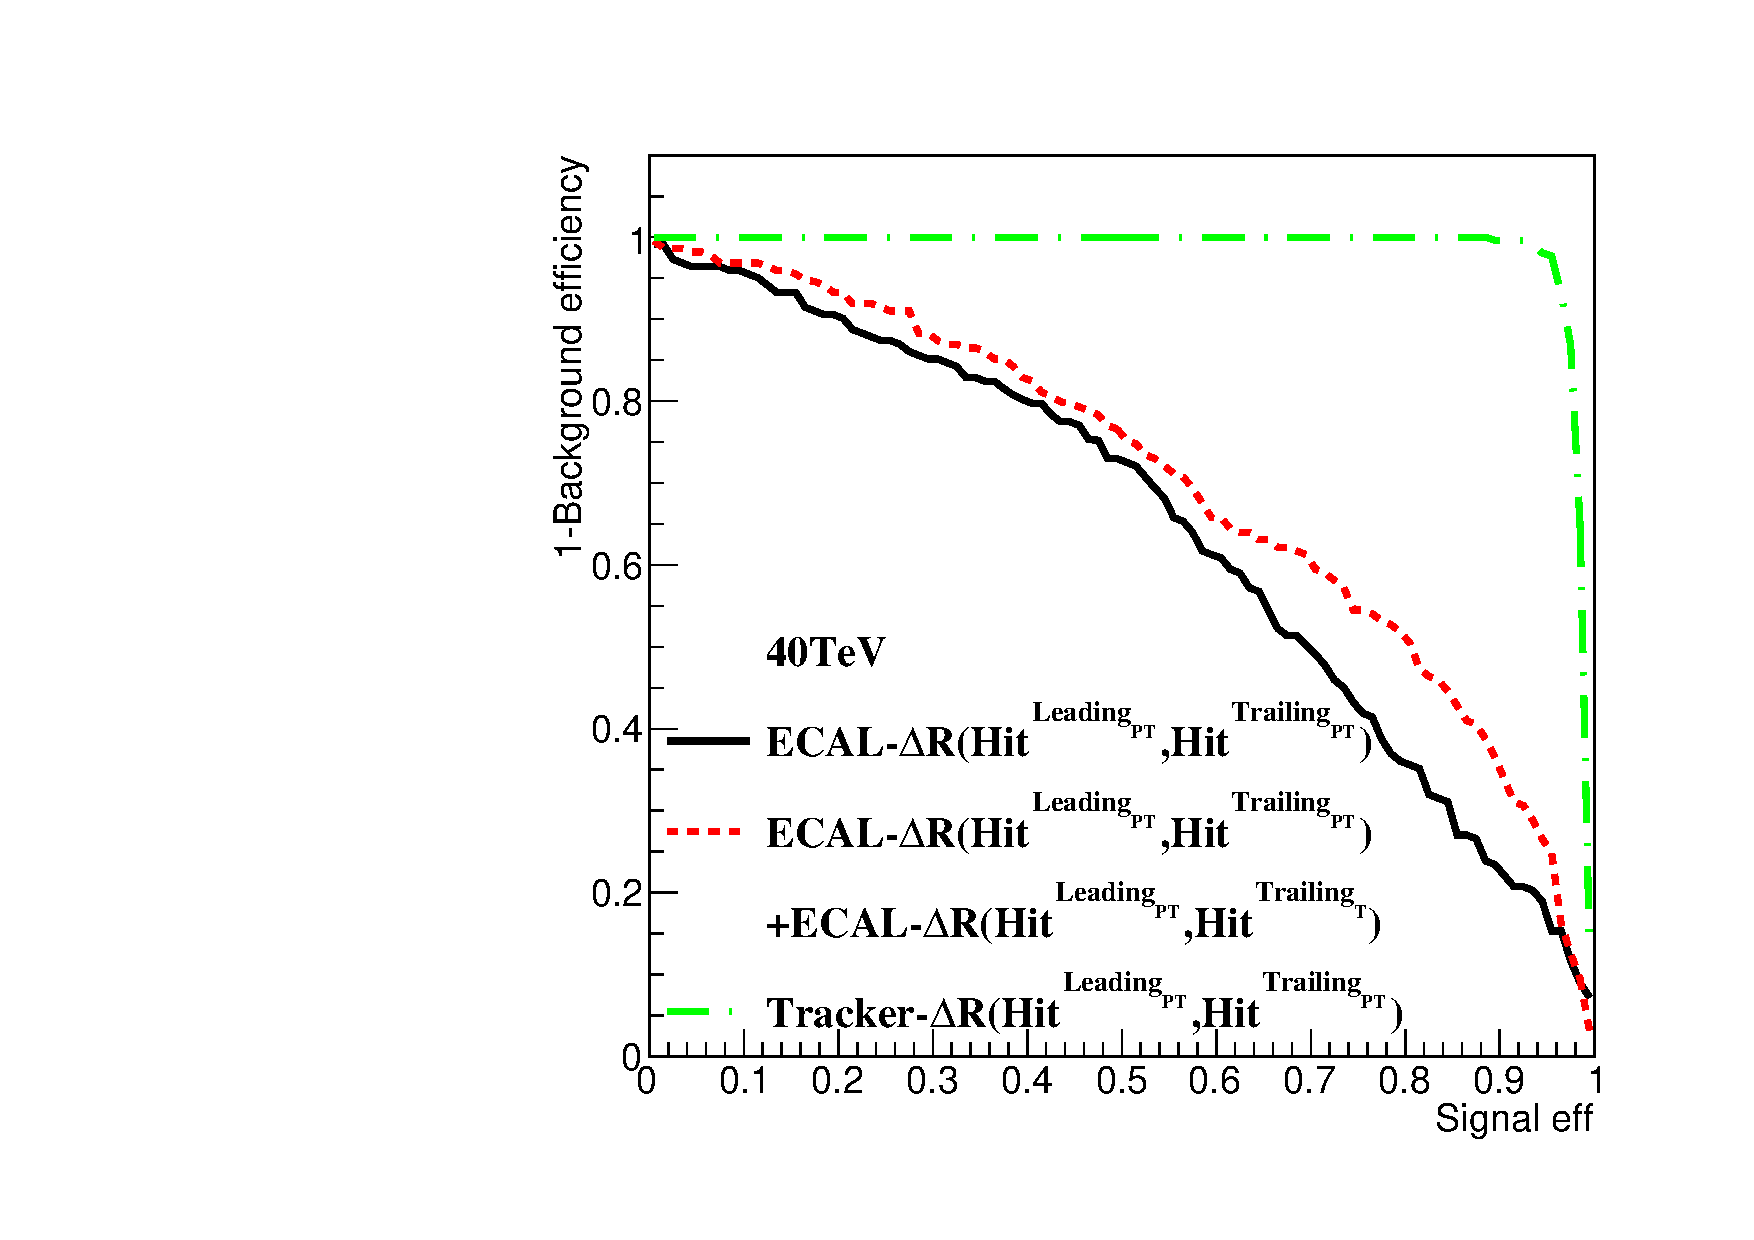
\includegraphics[width=0.4\textwidth]{/Users/ms08962476/Timing_paper/Pictures_used_for_FCC_and_jets/Reco_dR_BDT/BDT_plot_dR_dRplusID_40TeV_Reco.pdf}
   }
\end{center}
\caption{The comparison of the ROC curves obtained from two cases including five trailing-$P_{T}$ particles of ECAL up to the fifth order alone(black) and the ones accompanied by five trailing-T particles of ECAL up to the same order(red), as well we the one drawn with trailing-$P_{T}$ particles of the tracker up to the same order(green) with the reco-level information of the different $M(Z')$ are shown here. The signal (background) process is $Z'\rightarrow WW$ ($Z' \rightarrow q\bar{q}$). \label{fig:Reco_dR_BDT}}
\end{figure}

Speaking of the $\Delta R$ which is strongly-dependent of the precise of measuring the momenta, the tracker, which can get rid of the issue on non-smearing problem as ECAL to explicitly measure the momentum with the high-granularity cell, is the essential detector to explore the efficiency of the parameter. The distributions of $\Delta R$ with the tracker are posted in Fig.\ref{fig:Tracker_Reco_dR_Dis_5TeV_PT} and Fig.\ref{fig:Tracker_Reco_dR_Dis_40TeV_PT}, that show the cases are very similar to the truth-level ones as if the precise four momenta can be sought out, the better separation between two different number of subjets can be discovered. As the schemes of BDT plots shown in Fig.\ref{fig:Reco_dR_BDT} as the one mentioned in the previous paragraph, the line obtained from the tracker with the trailing-$P_{T}$ particles up to the fifth order shows that the high-rejection of the background with the accurate measurement of the four momenta can be used as the mean to complete the task of distinguishing the different number of subjet. \footnote{At the moment, since the timing information from the tracker in our current simulation can't be acquired as another detectors, we only apply the trailing-$P_{T}$ for the tracker case.}\\

\begin{figure}
\begin{center}
   \subfigure[The first trailing-T] {
   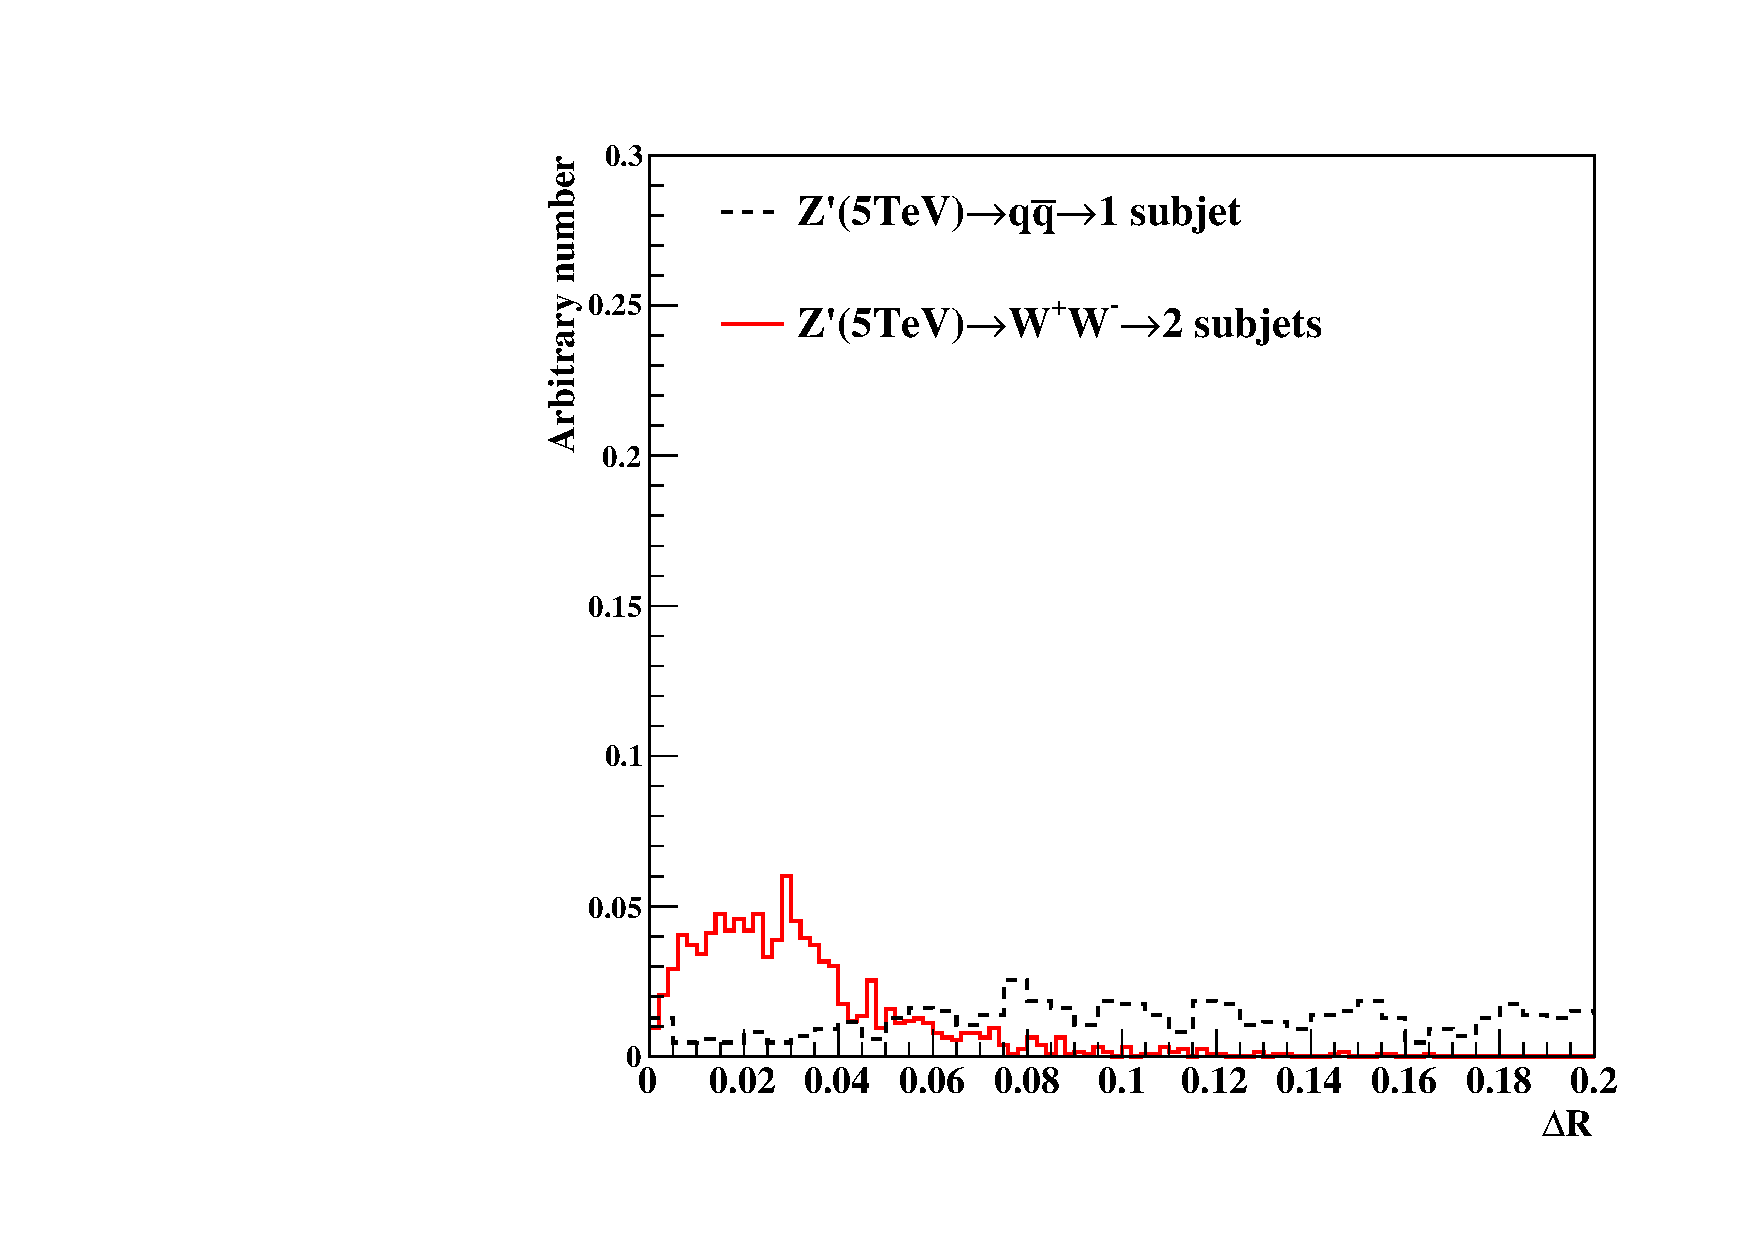
\includegraphics[width=0.3\textwidth]{/Users/ms08962476/Timing_paper/Pictures_used_for_FCC_and_jets/Reco_dR_Dis_Tracker/5TeV_Reco_track/dR_PT_0_5TeV_Reco_track.pdf}
   }
   \subfigure[The second trailing-T] {
   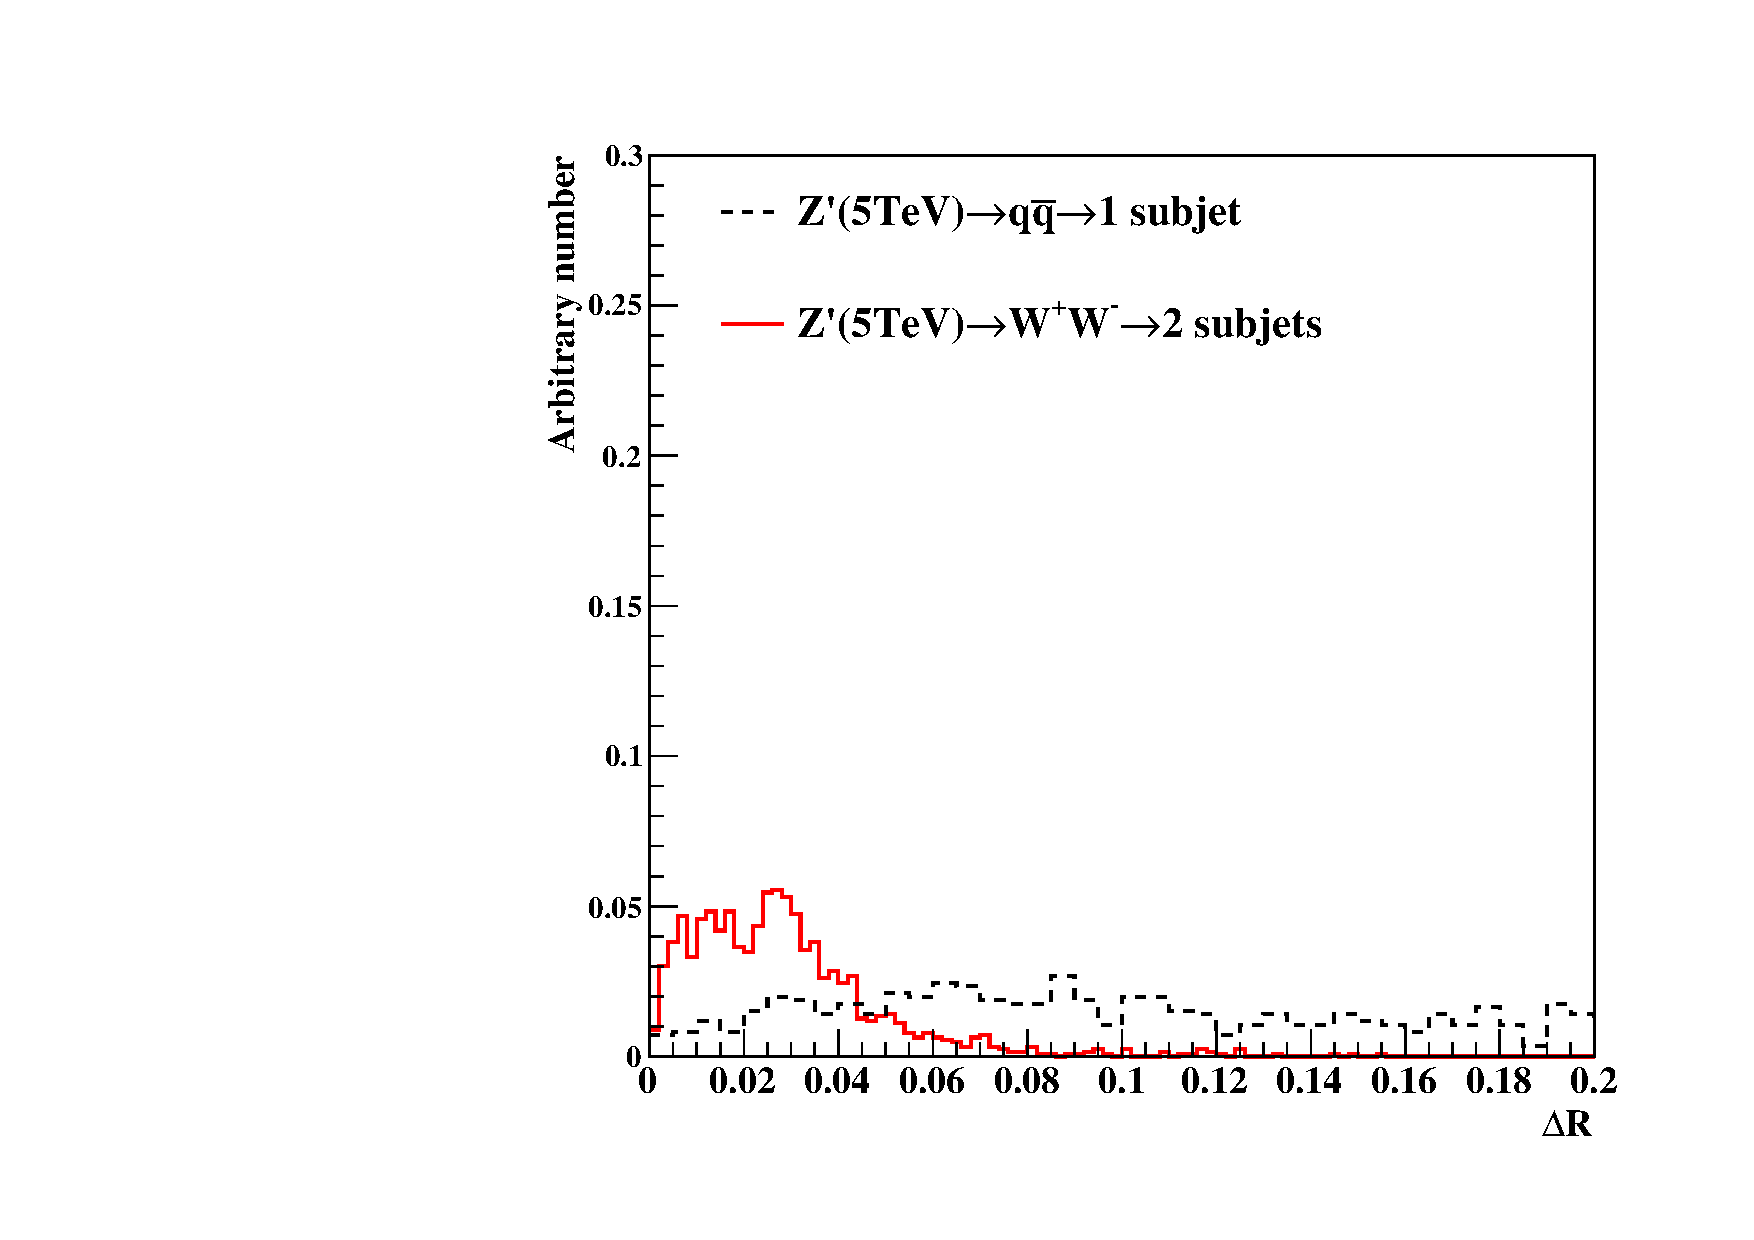
\includegraphics[width=0.3\textwidth]{/Users/ms08962476/Timing_paper/Pictures_used_for_FCC_and_jets/Reco_dR_Dis_Tracker/5TeV_Reco_track/dR_PT_1_5TeV_Reco_track.pdf}
   }
   \subfigure[The third trailing-T] {
   \includegraphics[width=0.3\textwidth]{/Users/ms08962476/Timing_paper/Pictures_used_for_FCC_and_jets/Reco_dR_Dis_Tracker/5TeV_Reco_track/dR_PT_2_5TeV_Reco_track.pdf}
   }
      \subfigure[The fourth trailing-T] {
   \includegraphics[width=0.3\textwidth]{/Users/ms08962476/Timing_paper/Pictures_used_for_FCC_and_jets/Reco_dR_Dis_Tracker/5TeV_Reco_track/dR_PT_3_5TeV_Reco_track.pdf}
   }
   \subfigure[The fifth trailing-T] {
   \includegraphics[width=0.3\textwidth]{/Users/ms08962476/Timing_paper/Pictures_used_for_FCC_and_jets/Reco_dR_Dis_Tracker/5TeV_Reco_track/dR_PT_4_5TeV_Reco_track.pdf}
   }
\end{center}
\caption{Distributions of $\Delta R$ for $M(Z') = 5$~TeV for five kinds of trailing-$P_{T}$ particles with the reco-level information of tracker
are shown here. \label{fig:Tracker_Reco_dR_Dis_5TeV_PT}}
\end{figure}

\begin{figure}
\begin{center}
   \subfigure[The first trailing-T] {
   \includegraphics[width=0.3\textwidth]{/Users/ms08962476/Timing_paper/Pictures_used_for_FCC_and_jets/Reco_dR_Dis_Tracker/40TeV_Reco_track/dR_PT_0_40TeV_Reco_track.pdf}
   }
   \subfigure[The second trailing-T] {
   \includegraphics[width=0.3\textwidth]{/Users/ms08962476/Timing_paper/Pictures_used_for_FCC_and_jets/Reco_dR_Dis_Tracker/40TeV_Reco_track/dR_PT_1_40TeV_Reco_track.pdf}
   }
   \subfigure[The third trailing-T] {
   \includegraphics[width=0.3\textwidth]{/Users/ms08962476/Timing_paper/Pictures_used_for_FCC_and_jets/Reco_dR_Dis_Tracker/40TeV_Reco_track/dR_PT_2_40TeV_Reco_track.pdf}
   }
      \subfigure[The fourth trailing-T] {
   \includegraphics[width=0.3\textwidth]{/Users/ms08962476/Timing_paper/Pictures_used_for_FCC_and_jets/Reco_dR_Dis_Tracker/40TeV_Reco_track/dR_PT_3_40TeV_Reco_track.pdf}
   }
   \subfigure[The fifth trailing-T] {
   \includegraphics[width=0.3\textwidth]{/Users/ms08962476/Timing_paper/Pictures_used_for_FCC_and_jets/Reco_dR_Dis_Tracker/40TeV_Reco_track/dR_PT_4_40TeV_Reco_track.pdf}
   }
\end{center}
\caption{Distributions of $\Delta R$ for $M(Z') = 40$~TeV for five kinds of trailing-$P_{T}$ particles with the reco-level information of tracker
are shown here. \label{fig:Tracker_Reco_dR_Dis_40TeV_PT}}
\end{figure}








%%%%%%%%%%%%%%% commented out 
%\end{comment}

